\documentclass[10pt,a4paper]{article}
%\usepackage[top=0.85in,left=2.75in,footskip=0.75in]{geometry}
\usepackage[english]{babel}
\usepackage[utf8x]{inputenc}
\usepackage[T1]{fontenc}
\usepackage[a4paper]{geometry}
\geometry{a4paper, top=1in, bottom=2in}
\usepackage{amsmath}
\usepackage{amssymb}
\usepackage{graphicx}
\usepackage[colorlinks=true, allcolors=blue, hypertexnames=false]{hyperref}
\usepackage{epsfig,amsfonts}
%\usepackage{natbib}
\usepackage{authblk}
\usepackage{subfig}
\usepackage{setspace}
\usepackage{hypcap}
\usepackage{lscape}
\usepackage{lineno} %can do [right] to shift location of #s
%From: https://www.overleaf.com/learn/how-to/Cross_referencing_with_the_xr_package_in_Overleaf
\usepackage{xr}
\makeatletter
\newcommand*{\addFileDependency}[1]{% argument=file name and extension
  \typeout{(#1)}
  \@addtofilelist{#1}
  \IfFileExists{#1}{}{\typeout{No file #1.}}
}
\makeatother
\newcommand*{\myexternaldocument}[1]{%
    \externaldocument{#1}%
    \addFileDependency{#1.tex}%
    \addFileDependency{#1.aux}%
}
\myexternaldocument{Main}
%From: https://tex.stackexchange.com/questions/64934/subfig-label-positioning (went with second example solution on how to get multiple figures aligned with subfig + desired labeling)
%\usepackage{floatrow}
%From: https://tex.stackexchange.com/questions/332295/command-textalpha-unavailable-in-encoding-t1-when-using-greek
\usepackage{textgreek}

%From Lorin
\usepackage{latexsym}
\usepackage{bm}
\usepackage{bbm}

\def\eq#1{(\ref{#1})}
\def\pdf{p.d.f.\ } \def\cdf{c.d.f.\ }
\def\pdfs{p.d.f.s} \def\cdfs{c.d.f.s}
\def\mgf{m.g.f.\ } \def\mgfs{m.g.f.s\ }
\def\ci{\perp   \perp}  % conditional independence symbol
\def\beginmat{ \left( \begin{array} }
\def\endmat{ \end{array} \right) }
\def\diag{{\rm diag}}
\def\log{{\rm log}}
\def\tr{{\rm tr}}
\def\cond{\, | \,}
\newcommand*\diff{\mathop{}\!\mathrm{d}}
%\newcolumntype{P}[1]{>{\centering\arraybackslash}p{#1}}

\newtheorem{claim}{Claim}[section]
\newtheorem{definition}{Definition}[section]
\newtheorem{thm}{Theorem}[section]
\newtheorem{prop}{Proposition}[section]

\def\dsum{\displaystyle\sum}
\def\dint{\displaystyle\int}
%\def\dfrac{\displaystyle\frac}
\def\dsup{\displaystyle\sup}
\def\dinf{\displaystyle\inf}
\def\dmin{\displaystyle\min}
\def\dlim{\displaystyle\lim}

\newcommand{\me}{\mathrm{e}}
\newcommand{\supp}{\operatorname{supp}}
\newcommand{\abs}[1]{\left|#1\right|}
\newcommand{\comment}[1]{{\em #1}}
\newcommand{\ba}{\mathbf{a}}
\newcommand{\bb}{\mathbf{b}}
\newcommand{\bc}{\mathbf{c}}
\newcommand{\be}{\mathbf{e}}
\newcommand{\bg}{\mathbf{g}}
\newcommand{\bl}{\mathbf{l}}
\newcommand{\bs}{\mathbf{s}}
\newcommand{\bq}{\mathbf{q}}
\newcommand{\bk}{\mathbf{k}}
\newcommand{\bv}{\mathbf{v}}
\newcommand{\bx}{\mathbf{x}}
\newcommand{\by}{\mathbf{y}}
\newcommand{\bz}{\mathbf{z}}
\newcommand{\bh}{\mathbf{h}}
\newcommand{\bu}{\mathbf{u}}
\newcommand{\bfm}{\mathbf{m}}
\newcommand{\bw}{\mathbf{w}}
\newcommand{\w}{\mathbf{w}}
\newcommand{\bp}{\mathbf{p}}
\newcommand{\bK}{\mathbf{K}}
\newcommand{\bV}{\mathbf{V}}
\newcommand{\bA}{\mathbf{A}}
\newcommand{\bB}{\mathbf{B}}
\newcommand{\bC}{\mathbf{C}}
\newcommand{\bX}{\mathbf{X}}
\newcommand{\bY}{\mathbf{Y}}
\newcommand{\bE}{\mathbf{E}}
\newcommand{\bG}{\mathbf{G}}
\newcommand{\bH}{\mathbf{H}}
\newcommand{\bP}{\mathbf{P}}
\newcommand{\bQ}{\mathbf{Q}}
\newcommand{\bR}{\mathbf{R}}
\newcommand{\bW}{\mathbf{W}}
\newcommand{\bM}{\mathbf{M}}
\newcommand{\bU}{\mathbf{U}}
\newcommand{\bZ}{\mathbf{Z}}
\newcommand{\bD}{\mathbf{D}}
\newcommand{\bI}{\mathbf{I}}
\newcommand{\bS}{\mathbf{S}}
\newcommand{\T}{\intercal}
\newcommand{\wt}{\widetilde}
\newcommand{\wh}{\widehat}

\newcommand{\E}{\mathbb{E}}
\newcommand{\V}{\mathbb{V}}

\newcommand{\bbE}{\mathbb{E}}
\newcommand{\bbV}{\mathbb{V}}
\newcommand{\N}{\mathcal{N}}

\newcommand{\bepsilon}{\boldsymbol\epsilon}
\newcommand{\bvarepsilon}{\boldsymbol\varepsilon}
\newcommand{\bbeta}{\boldsymbol\beta}
\newcommand{\bsigma}{\boldsymbol\sigma}
\newcommand{\tbbeta}{{\tilde{\boldsymbol\beta}}}
\newcommand{\tbeta}{{\tilde{\beta}}}
\newcommand{\bgamma}{\boldsymbol\gamma}
\newcommand{\bdelta}{\boldsymbol\delta}
\newcommand{\btheta}{\boldsymbol\theta}
\newcommand{\bpsi}{\boldsymbol\psi}
\newcommand{\bphi}{\boldsymbol\phi}
\newcommand{\brho}{\boldsymbol\rho}
\newcommand{\balpha}{\boldsymbol\alpha}
\newcommand{\bmu}{\boldsymbol\mu}
\newcommand{\bomega}{\boldsymbol\omega}
\newcommand{\btau}{\boldsymbol\tau}
\newcommand{\bDelta}{\boldsymbol\Delta}
\newcommand{\bOmega}{\boldsymbol\Omega}
\newcommand{\bSigma}{\boldsymbol\Sigma}
\newcommand{\bLambda}{\boldsymbol\Lambda}
\newcommand{\bTheta}{\boldsymbol\Theta}
\newcommand{\at}[2][]{#1|_{#2}}
\newcommand{\red}[1]{\textcolor{red}{#1}}
\newcommand{\blue}[1]{\textcolor{blue}{#1}}

%2020091 Additions from Lorin's main edits
\topmargin 0.0cm
\oddsidemargin 0.5cm
\evensidemargin 0.5cm
\textwidth 16cm 
\textheight 21cm

\usepackage{latexsym,color,multirow,soul,xspace,tabularx}
\usepackage{booktabs}
\usepackage{multirow,multicol}
\usepackage{grffile}
\usepackage{epstopdf}
\usepackage{longtable}
\usepackage{adjustbox} 
\usepackage{makecell}
\usepackage{sidecap}
\usepackage{algorithm}
\usepackage{algpseudocode}
\usepackage{tikz}
\usepackage{caption}
\usepackage[subfigure]{tocloft}
\usepackage{etoolbox}
\usepackage{pdflscape}
%\pagestyle{myheadings}

\newcommand{\edit}[2]{\sout{#1}\textcolor{red}{\xspace#2}}
%\newcommand{\sr}[2]{\sout{#1}\textcolor{red}{#2}}
\newcommand{\black}{\textcolor{black}}
\newcommand{\genee}{gene-$\varepsilon$~}
\newcommand{\genE}{gene-$\varepsilon$}

\DeclareMathOperator*{\argmin}{arg\,min}
\DeclareMathOperator*{\argmax}{arg\,max}

\newcolumntype{R}[2]{%
    >{\adjustbox{angle=#1,lap=\width-(#2)}\bgroup}%
    l%
    <{\egroup}%
}
\newcommand*\rot{\multicolumn{1}{R{90}{1em}}}
\newcolumntype{P}[1]{>{\centering\arraybackslash}p{#1}}

\allowdisplaybreaks

\renewcommand\thesubfigure{(\Alph{subfigure})}

\bibliographystyle{plos2015}

% Remove brackets from numbering in List of References
\makeatletter
\renewcommand{\@biblabel}[1]{\quad#1.}
\makeatother


%%%%%%%%%%%%
%%%%%%%%%%%%

\title{Supplementary: Differential complex trait architecture across humans: epistasis identified in non-European populations at multiple genomic scales}
\author[1,2]{Michael C. Turchin}
\author[1,3]{Isabella Ting}
\author[1,4,5,*]{Lorin Crawford}
\author[1,2,*,$\dag$]{Sohini Ramachandran}
\affil[1]{Center for Computational Molecular Biology, Brown University}
\affil[2]{Department of Ecology and Evolutionary Biology, Brown University}
\affil[3]{Department of Computer Science, Brown University}
\affil[4]{Department of Biostatistics, Brown University}
\affil[5]{Center for Statistical Science, Brown University}
\affil[$\ast$]{indicates these authors contributed equally}
\affil[$^\dag$]{To whom correspondence should be addressed: sramachandran@brown.edu}

\begin{document}
%\maketitle

% Title must be 150 characters or less
\begin{flushleft}
{\Large{\textbf{Supplementary Note to ``Pathway Analysis within Multiple Human Ancestries Reveals Novel Signals for Epistasis in Complex Traits''}}}
\newline
% Insert Author names, affiliations and corresponding author email.
\\
Michael C. Turchin\textsuperscript{1,2,$\dagger$}, Gregory Darnell\textsuperscript{2,3}, Lorin Crawford\textsuperscript{2,4,5,*}, and Sohini Ramachandran\textsuperscript{1,2,*,$\dagger$} 
\\
\bigskip
\bf{1} Department of Ecology and Evolutionary Biology, Brown University, Providence, RI, USA
\\
\bf{2} Center for Computational Molecular Biology, Brown University, Providence, RI, USA
\\
\bf{3} Institute for Computational and Experimental Research in Mathematics (ICERM), Brown University, Providence, RI, USA
\\
\bf{4} Department of Biostatistics, Brown University, Providence, RI, USA
\\
\bf{5} Center for Statistical Sciences, Brown University, Providence, RI, USA
\\
\bigskip
*: Authors Contributed Equally\\
$\dagger$ Corresponding E-mail: michael\_turchin@brown.edu; sramachandran@brown.edu 
\end{flushleft}

\setcounter{figure}{0}
\setcounter{table}{0}
\setcounter{equation}{0}
\makeatletter 

\tableofcontents

\clearpage
\newpage

%\section{Supplementary Note}\label{Supplementary-Note}

\section{Data Quality Control Procedures for UK Biobank}

The results presented in the main text made use of genotyped chip data released from the UK Biobank \cite{Sudlow2015}. Here, we focus on subgroups in the UK Biobank included individuals based on their self-identified ancestries: ``African'', ``British'', ``Caribbean'', ``Chinese'', ``Indian'', and ``Pakistani'', respectively. Quality control procedures for each of these subgroups in the data are as follows. First, we removed (\textit{i}) SNPs with minor allele frequency (MAF) less than 1\%, (\textit{ii}) SNPs with missingness greater than 5\%, and (\textit{iii}) SNPs not in Hardy-Weinberg Equilibrium (Fisher's exact test $P > 10^{-6}$). We also removed individuals by checking three sets of criteria. First, we removed individuals if they were a 3rd degree relative (or more) to someone else in the dataset --- specifically, the KING relatedness values provided with the UK Biobank data were used to identify related individuals, and one individual from every pair of 3rd degree or more relatives was removed. Second, individuals were also removed if they were tagged by any of the following three flags within the UK Biobank data: \texttt{het.missing.outliers}, \texttt{putative.sex.chromosome.aneuploidy}, and \texttt{excess.relatives}. Lastly, individuals were removed if they were determined to be outliers via principal component analysis (PCA) --- this was conducted by running \texttt{FlashPCA} (version 2.1) \cite{Abraham2017} in \texttt{R} on each population subgroup separately and identifying individuals that had any of their top six principal component (PC) values greater than seven standard deviations away from the mean. We refer to conducting PCA on each subgroup separately as ``local PCA'' to help distinguish from the alternative setup of conducting PCA on the entire dataset jointly, which would be referred to as ``global PCA''. 

After the first round of quality control procedures, we then proceeded to impute missing genotypes for each population subgroup. To conduct this imputation, we uploaded our population subgroups to the University of Michigan Imputation Server \cite{Das2016} and used the following options: \texttt{Minimac3} for the imputation software, 1000 Genomes (phase 3 version 5) for the reference panel, and \texttt{Eagle} (version 2.3) for the phasing software. Completed imputed files were then downloaded from the Imputation Server afterwards and treated to one last round of quality control. Here, imputed variants were intersected back to the original set of genotyped chip variants. Variants with imputation quality scores  less than 30\% were removed, and variants that had genotype missingness greater than 0\% were also removed. Information on the final forms of our UK Biobank population subgroups can be found in Supplementary Table \ref{InterPath-Supp-Table-UKBPopStats}.

\section{Hypergeometric Enrichment Analyses}

Hypergeometric analyses were conducted by counting the number of times a given gene is present among the significant pathways identified by MAPIT-R for a given database-phenotype-subgroup combination versus the number of times the gene is present among the background distribution of pathways from the same database. For the size-restriction analyses, pathways with greater than 1,000 SNPs were removed. The 1,000 SNP threshold was chosen to balance between the total number of pathways removed and the average pathway size across all subgroups (see Supplementary Figure \ref{InterPath-Supp-Figure-pValsVsNumSNPs} for the relationship between MAPIT-R $P$-values and pathway sizes). Note that for a number of size thresholds ranging from 500 to 1,500 SNPs, results regarding the proteasome family genes remain robust (Supplementary Figure \ref{InterPath-Supp-Figure-Hypergeoemtric-SizeThresholds}).

\clearpage

\section{Supplementary Figures}\label{Supplementary-Figures}

%\renewcommand{\thefigure}{Supplementary Figure \arabic{figure}}
%\renewcommand{\thetable}{Supplementary \arabic{table}}
\renewcommand{\figurename}{Supplementary Figure}
\renewcommand{\tablename}{Supplementary Table}
\setcounter{figure}{0}
\setcounter{table}{0}

\begin{figure}[htbp]
\centering
%\hspace*{-1cm}
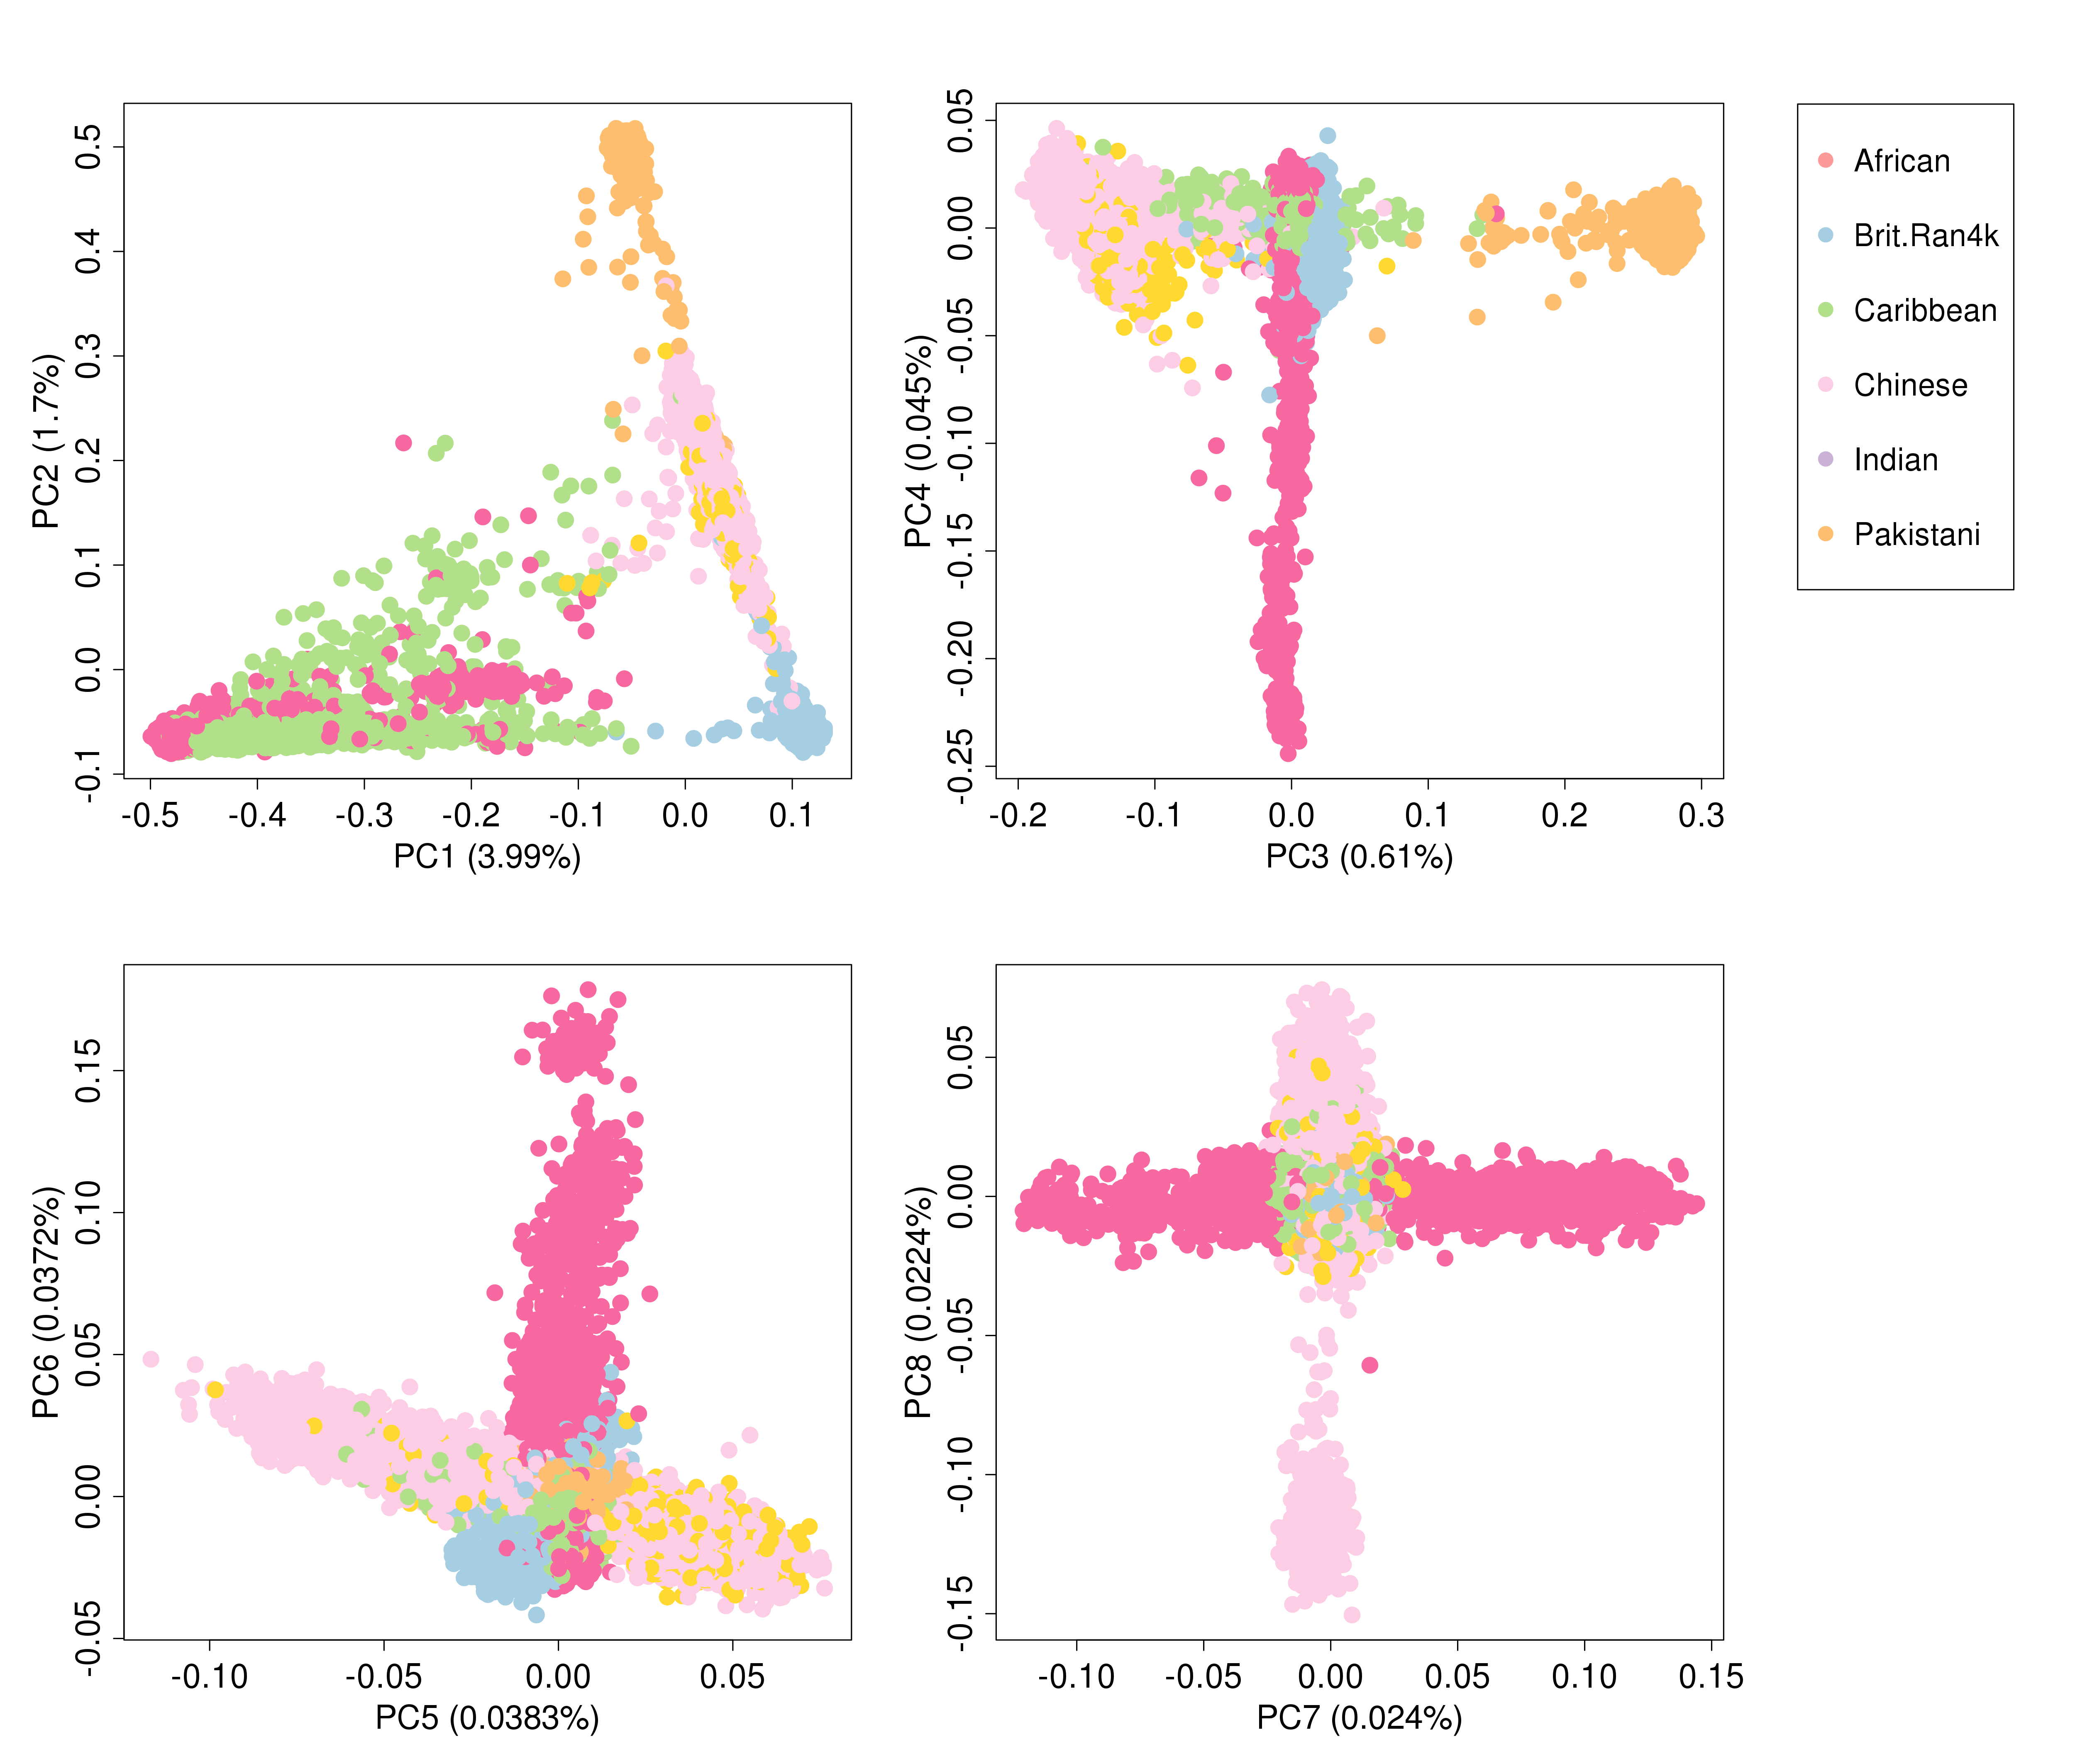
\includegraphics[width = \textwidth]{Images/Supp/InterPath_Supp_Figure_UKB_PCAPlot_vs2.png}
\caption{\textbf{Global principal component analysis (PCA) of the different ancestry-specific subgroups in the UK Biobank}. Here, subgroups in the UK Biobank included individuals based on their self-identified ancestries: ``African'', ``British'', ``Caribbean'', ``Chinese'', ``Indian'', and ``Pakistani'', respectively. The figure shows the top eight global principal components (PCs) for each subgroup plotted against one another. The comparisons include: \textbf{(a)} PC1 vs.~PC2, \textbf{(b)} PC3 vs.~PC4, \textbf{(c)} PC5 vs.~PC6, and \textbf{(d)} PC7 vs.~PC8. PCA was conducted using \texttt{FlashPCA} \cite{Abraham2017}. Here, ``global'' refers to running PCA on the full UK Biobank dataset with all subgroups pulled together jointly. This is in contrast to `local' PCA which conducts principal component analysis on each subgroup separately. Note that global PCs was only used for exploratory analyses and to create these plots, while local PCs were used for quality control and to adjust for population structure in the MAPIT-R analyses. On each axis, we also list the percent of total variation explained (PVE) by each PC in parentheses.}
\label{InterPath-Supp-Figure-UKB-subgroups-PCAPlot}
\end{figure}
\clearpage

\begin{figure}[htbp]
\centering
%\hspace*{-.9cm}
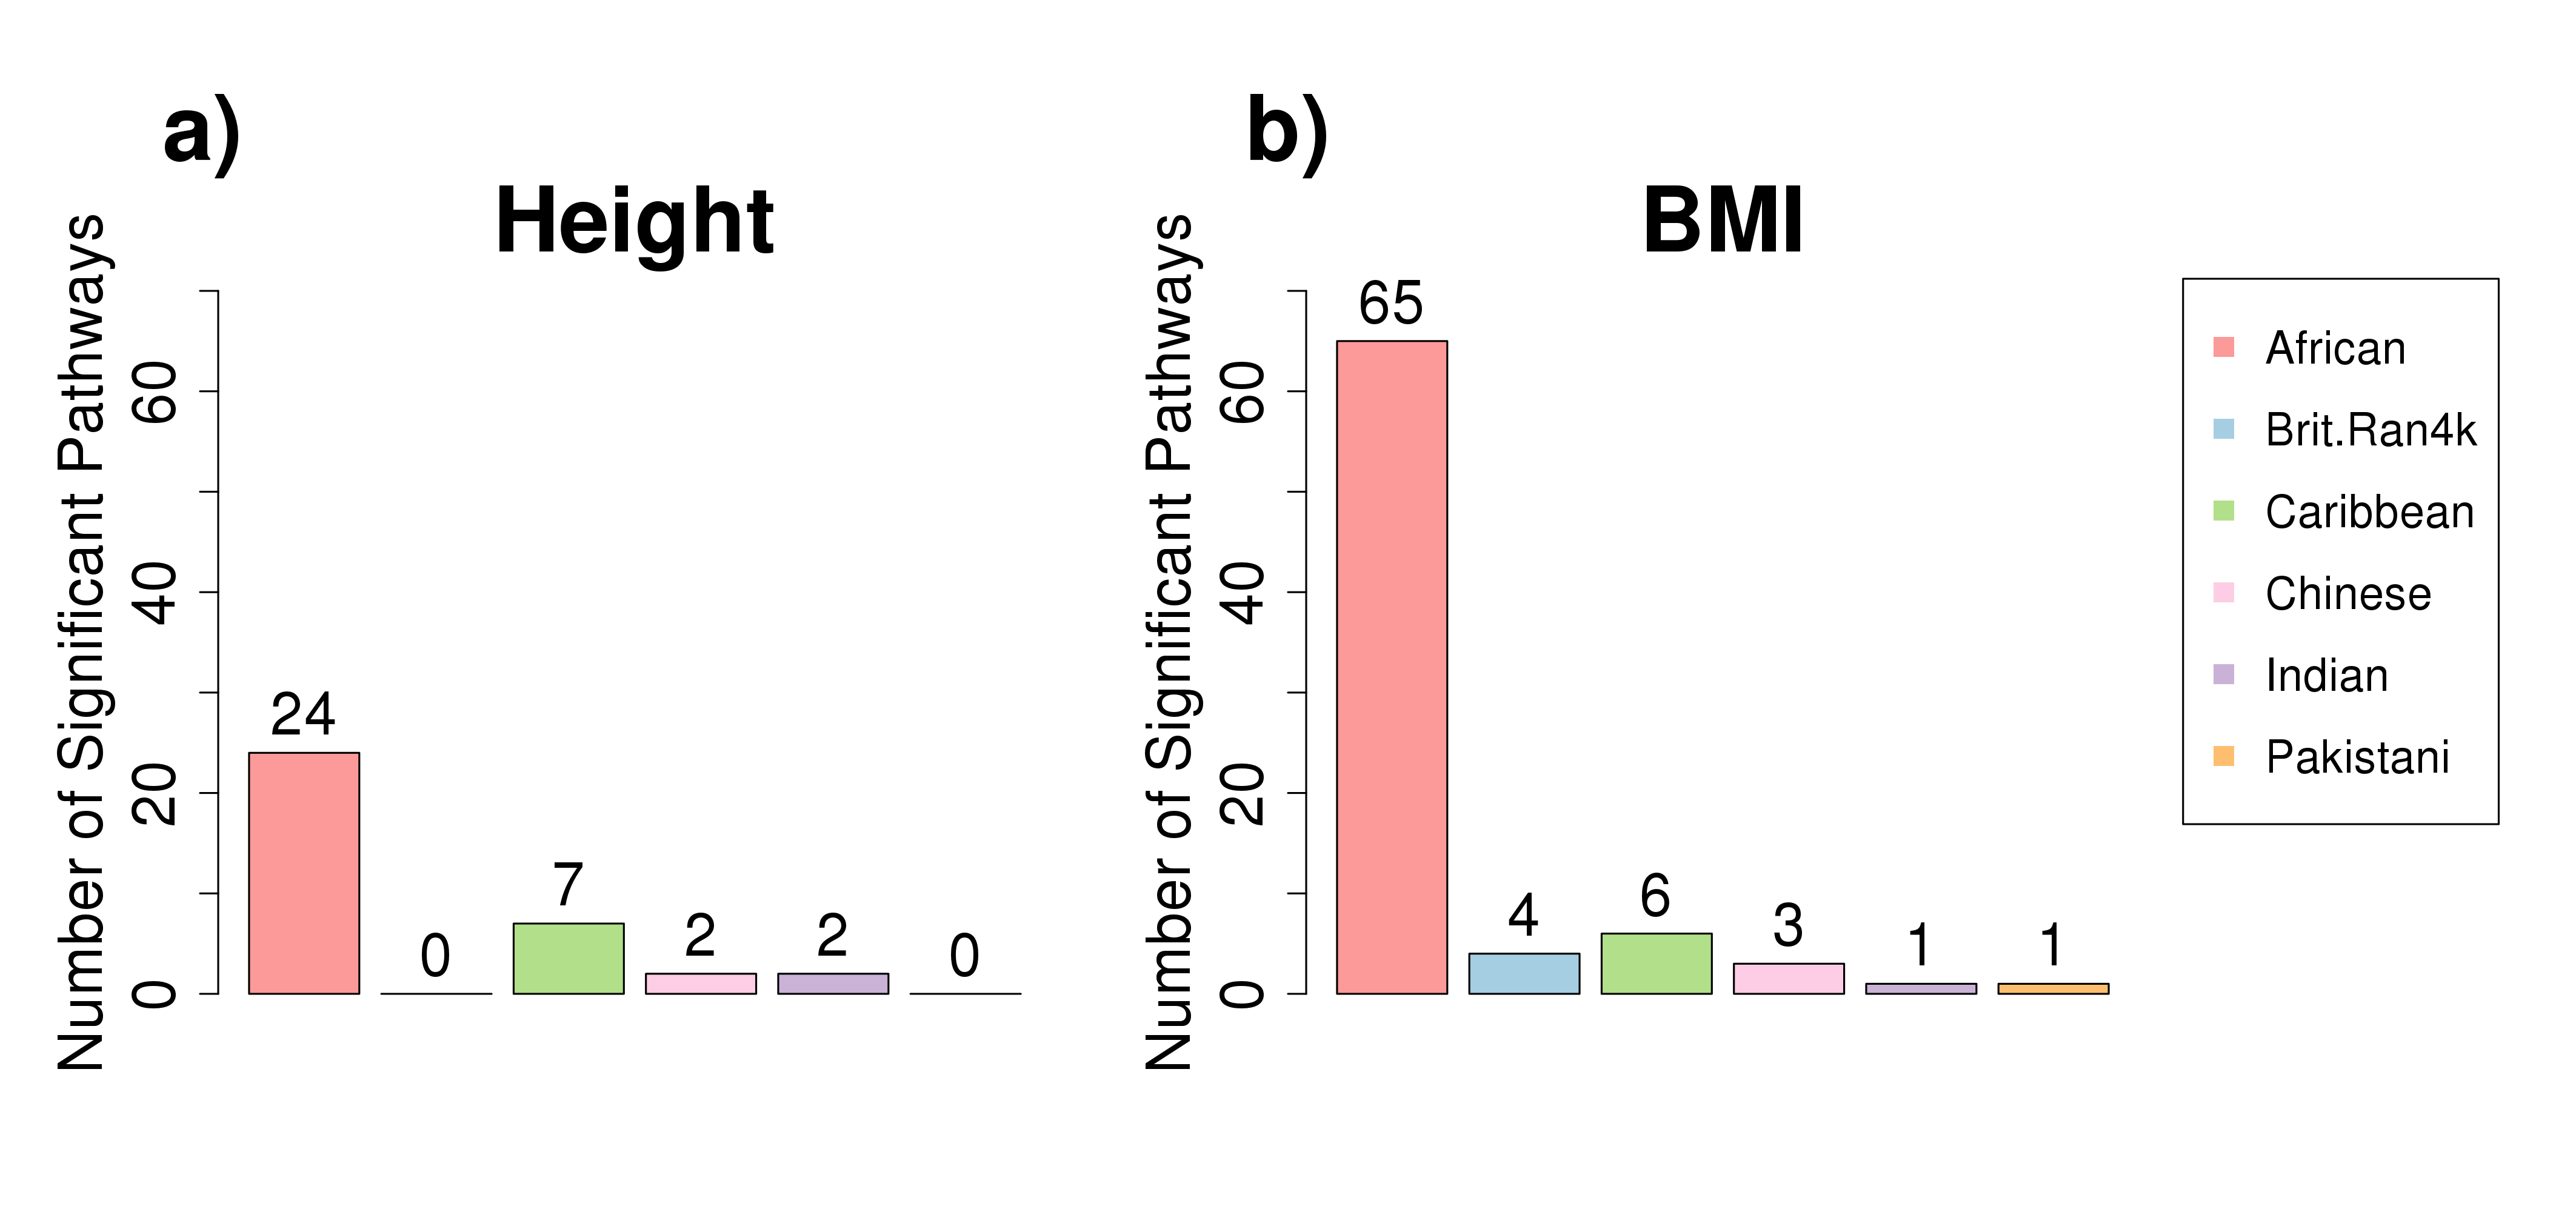
\includegraphics[width = \textwidth]{Images/Supp/InterPath_Supp_Figure_Barplots_REACTOME_vs4.png}
\caption{\textbf{Number of REACTOME pathways identified by MAPIT-R that have significant marginal epistatic effects within (a) standing height and (b) body mass index (BMI) per subgroup in the UK Biobank.} Here, the subgroups in the UK Biobank included individuals based on their self-identified ancestries: ``African'', ``British'', ``Caribbean'', ``Chinese'', ``Indian'', and ``Pakistani'', respectively. Genome-wide significance was determined by using Bonferroni-corrected $P$-value thresholds based on the number of pathways tested in each database-phenotype-subgroup combination (see Supplementary Table \ref{InterPath-Supp-Table-UKBPopStats}). Across all database-phenotype combinations, the African subgroup has the largest numbers of significant pathways. For lists of the specific significant pathways per database-phenotype-subgroup combination, see Supplementary Table \ref{InterPath-Supp-Table-TopPathways-AllPaths-AllPhenos}.}
\label{InterPath-Supp-Figure-Barplots-REACTOME}
\end{figure}
\clearpage

\begin{figure}[htbp]
\centering
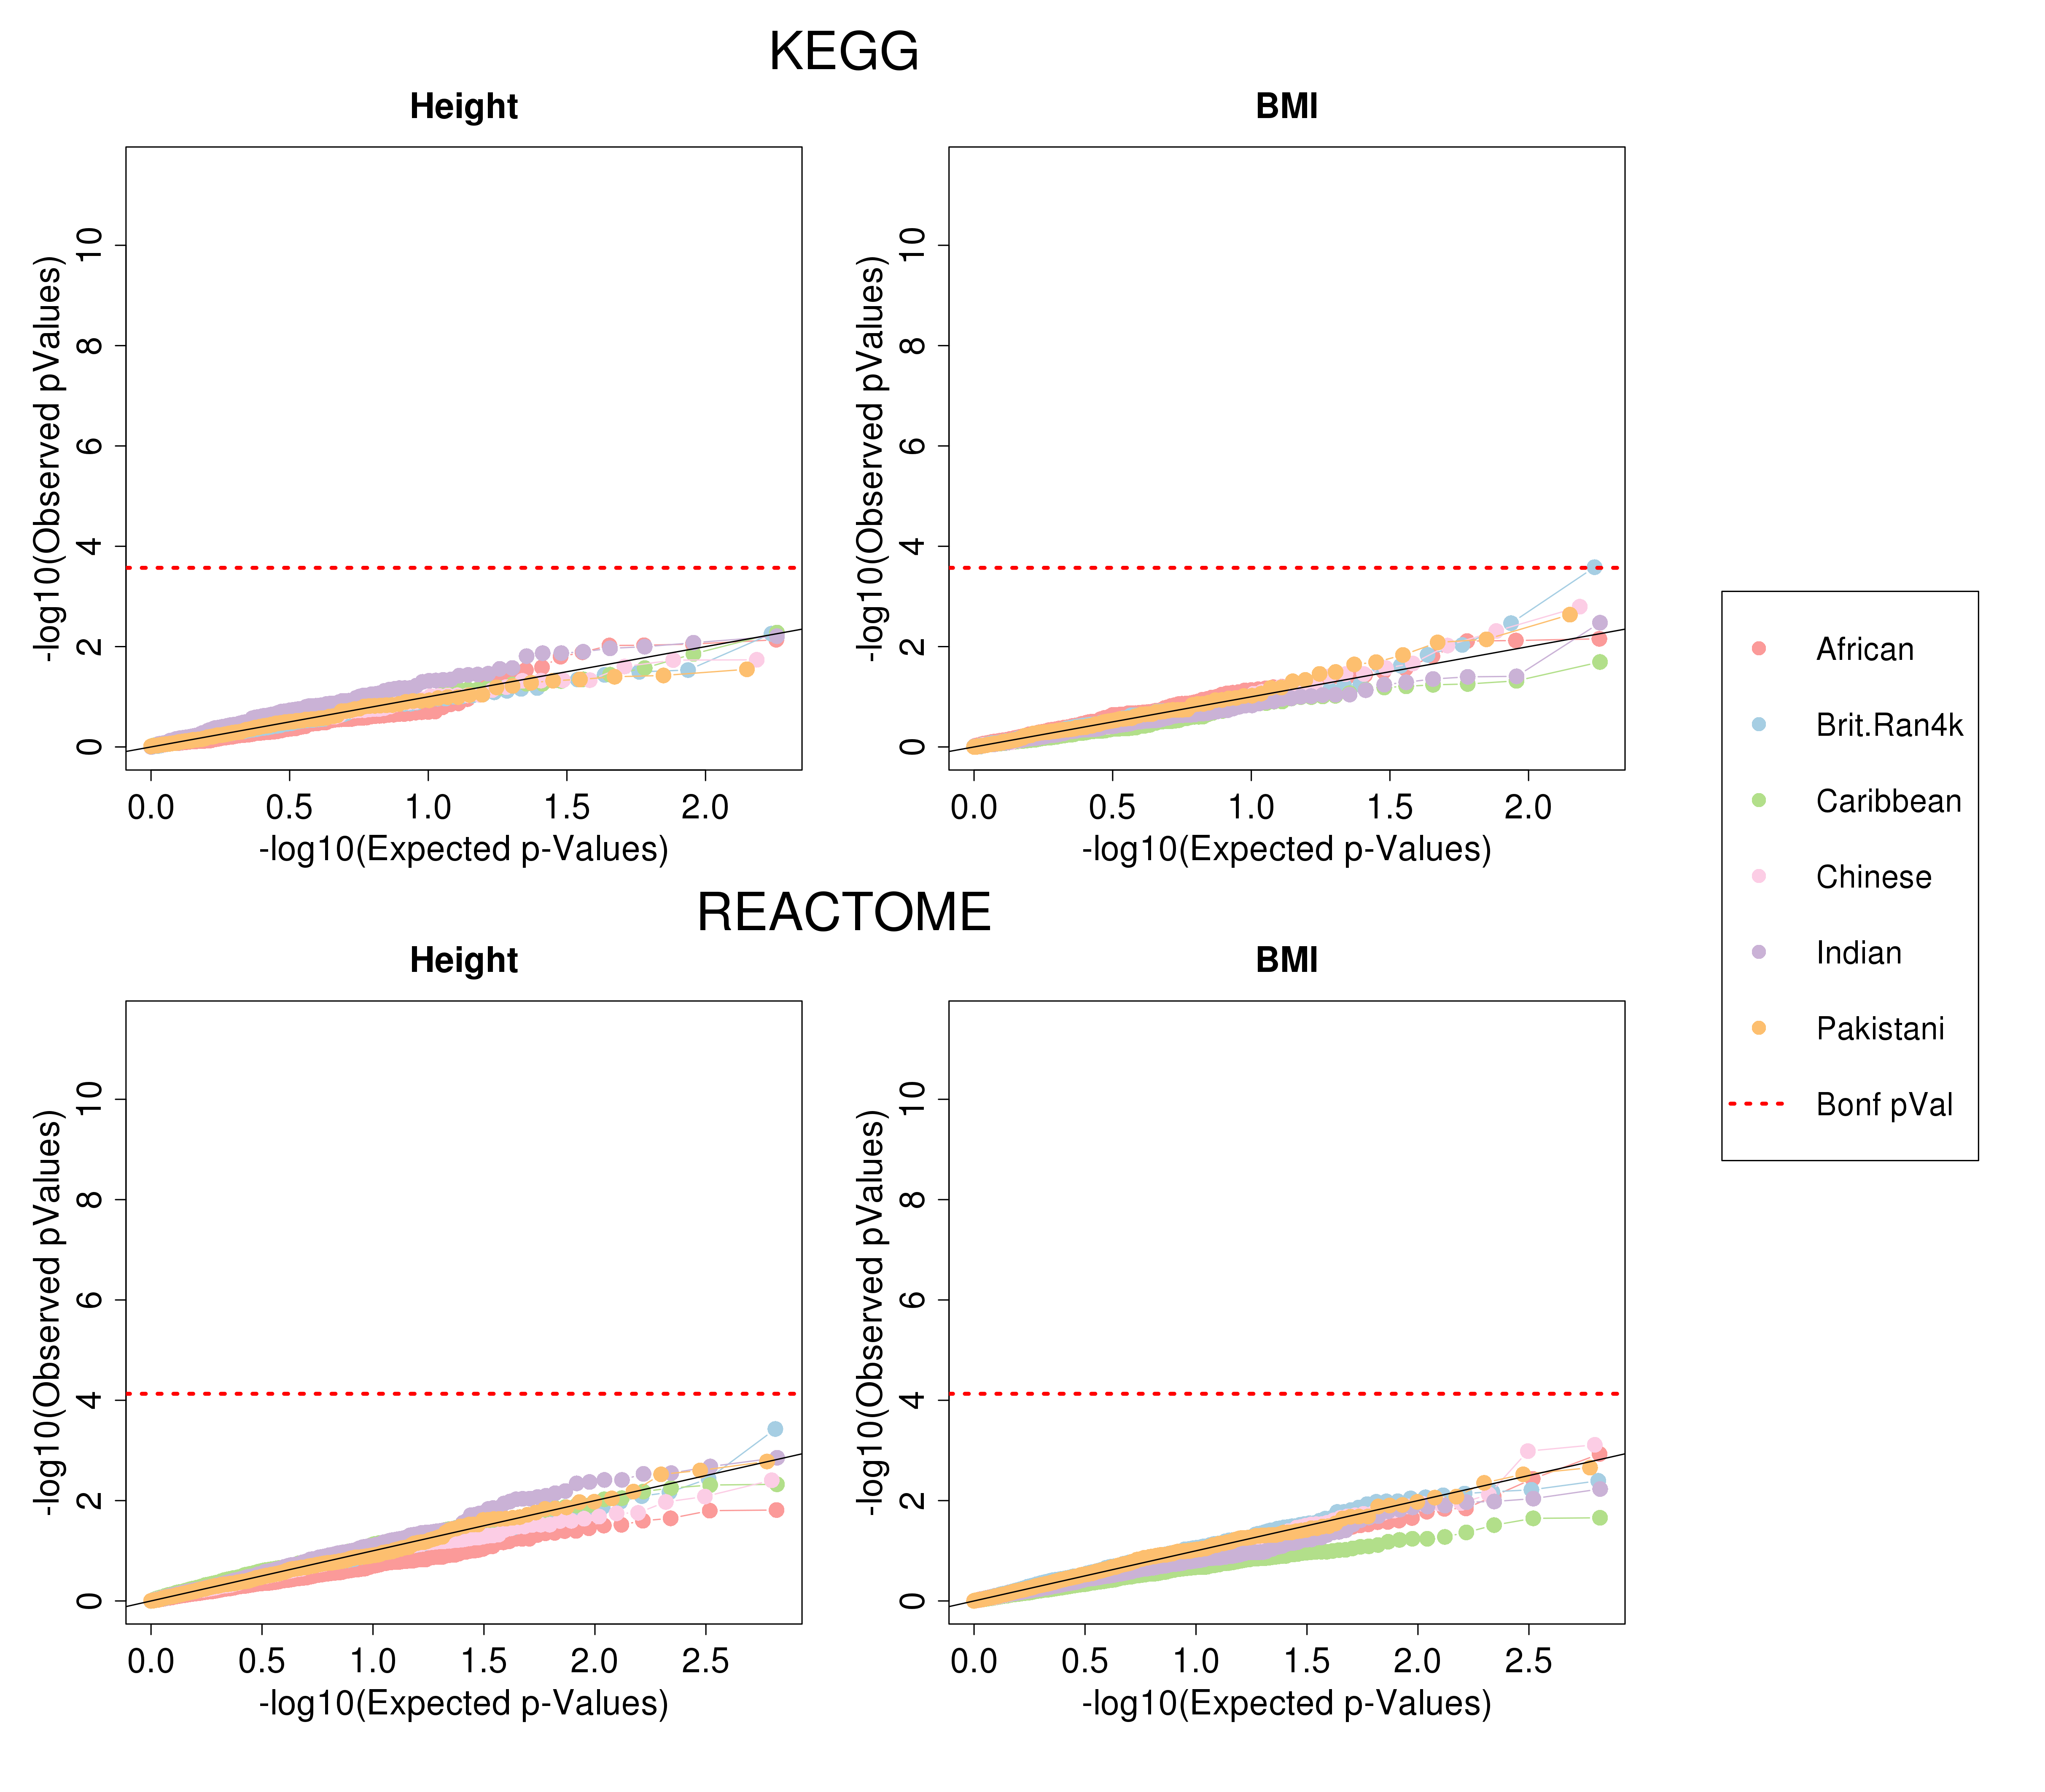
\includegraphics[width = \textwidth]{Images/Supp/InterPath_Supp_Figure_perm1_QQPlots_AllPaths_vs2.png}
\caption{\textbf{QQ-Plots of MAPIT-R $\bm{P}$-values using KEGG and REACTOME pathways annotations and randomly permuted phenotypes in each ancestry-specific subgroup in the UK Biobank.} Here, we run MAPIT-R after conducting a single random permutation of either height or BMI measurements. Note that traits were permuted within each population subgroup ten different times. Shown on the x-axis are the -$\log_{10}$ transformed expected $p$-values, while the $y$-axis shows the -$\log_{10}$ observed $p$-values. The dotted red line is the Bonferroni-corrected $P$-value threshold based on the number of pathways tested per database-phenotype combination (Supplementary Table \ref{InterPath-Supp-Table-UKBPopStats}). Subgroups in the UK Biobank included individuals based on their self-identified ancestries: ``African'', ``British'', ``Caribbean'', ``Chinese'', ``Indian'', and ``Pakistani'', respectively. Overall, we find that MAPIT-R properly controls for type 1 error rate at varying significance cutoff thresholds (Supplementary Table \ref{InterPath-Supp-Table-AllPops-FDRs}).}
\label{InterPath-Supp-Figure-perm1-QQPlots-AllPaths}
\end{figure}
\clearpage

\setlength{\footskip}{3cm}
\begin{figure}[htbp]
\centering
%\vspace*{-2cm}
\includegraphics[width = \textwidth]{Images/Supp/InterPath_Supp_Figure_pValHists_vs3.png}
\caption{\textbf{Histograms of MAPIT-R $\bm{p}$-values using KEGG and REACTOME pathways annotations and randomly permuted phenotypes in each ancestry-specific subgroup in the UK Biobank.} Here, we run MAPIT-R after conducting a single random permutation of either height or BMI measurements. Note that traits were independently permuted within each population subgroup ten different times. Subgroups in the UK Biobank included individuals based on their self-identified ancestries: ``African'', ``British'', ``Caribbean'', ``Chinese'', ``Indian'', and ``Pakistani'', respectively. Overall, we find that MAPIT-R properly controls for type 1 error rate at varying significance cutoff thresholds (Supplementary Table \ref{InterPath-Supp-Table-AllPops-FDRs}).}
\label{InterPath-Supp-Figure-10perms-pValHists}
\end{figure}
\clearpage
\setlength{\footskip}{1cm}

\setlength{\footskip}{1cm}
\begin{figure}[htbp]
\centering
%\vspace*{-2cm}
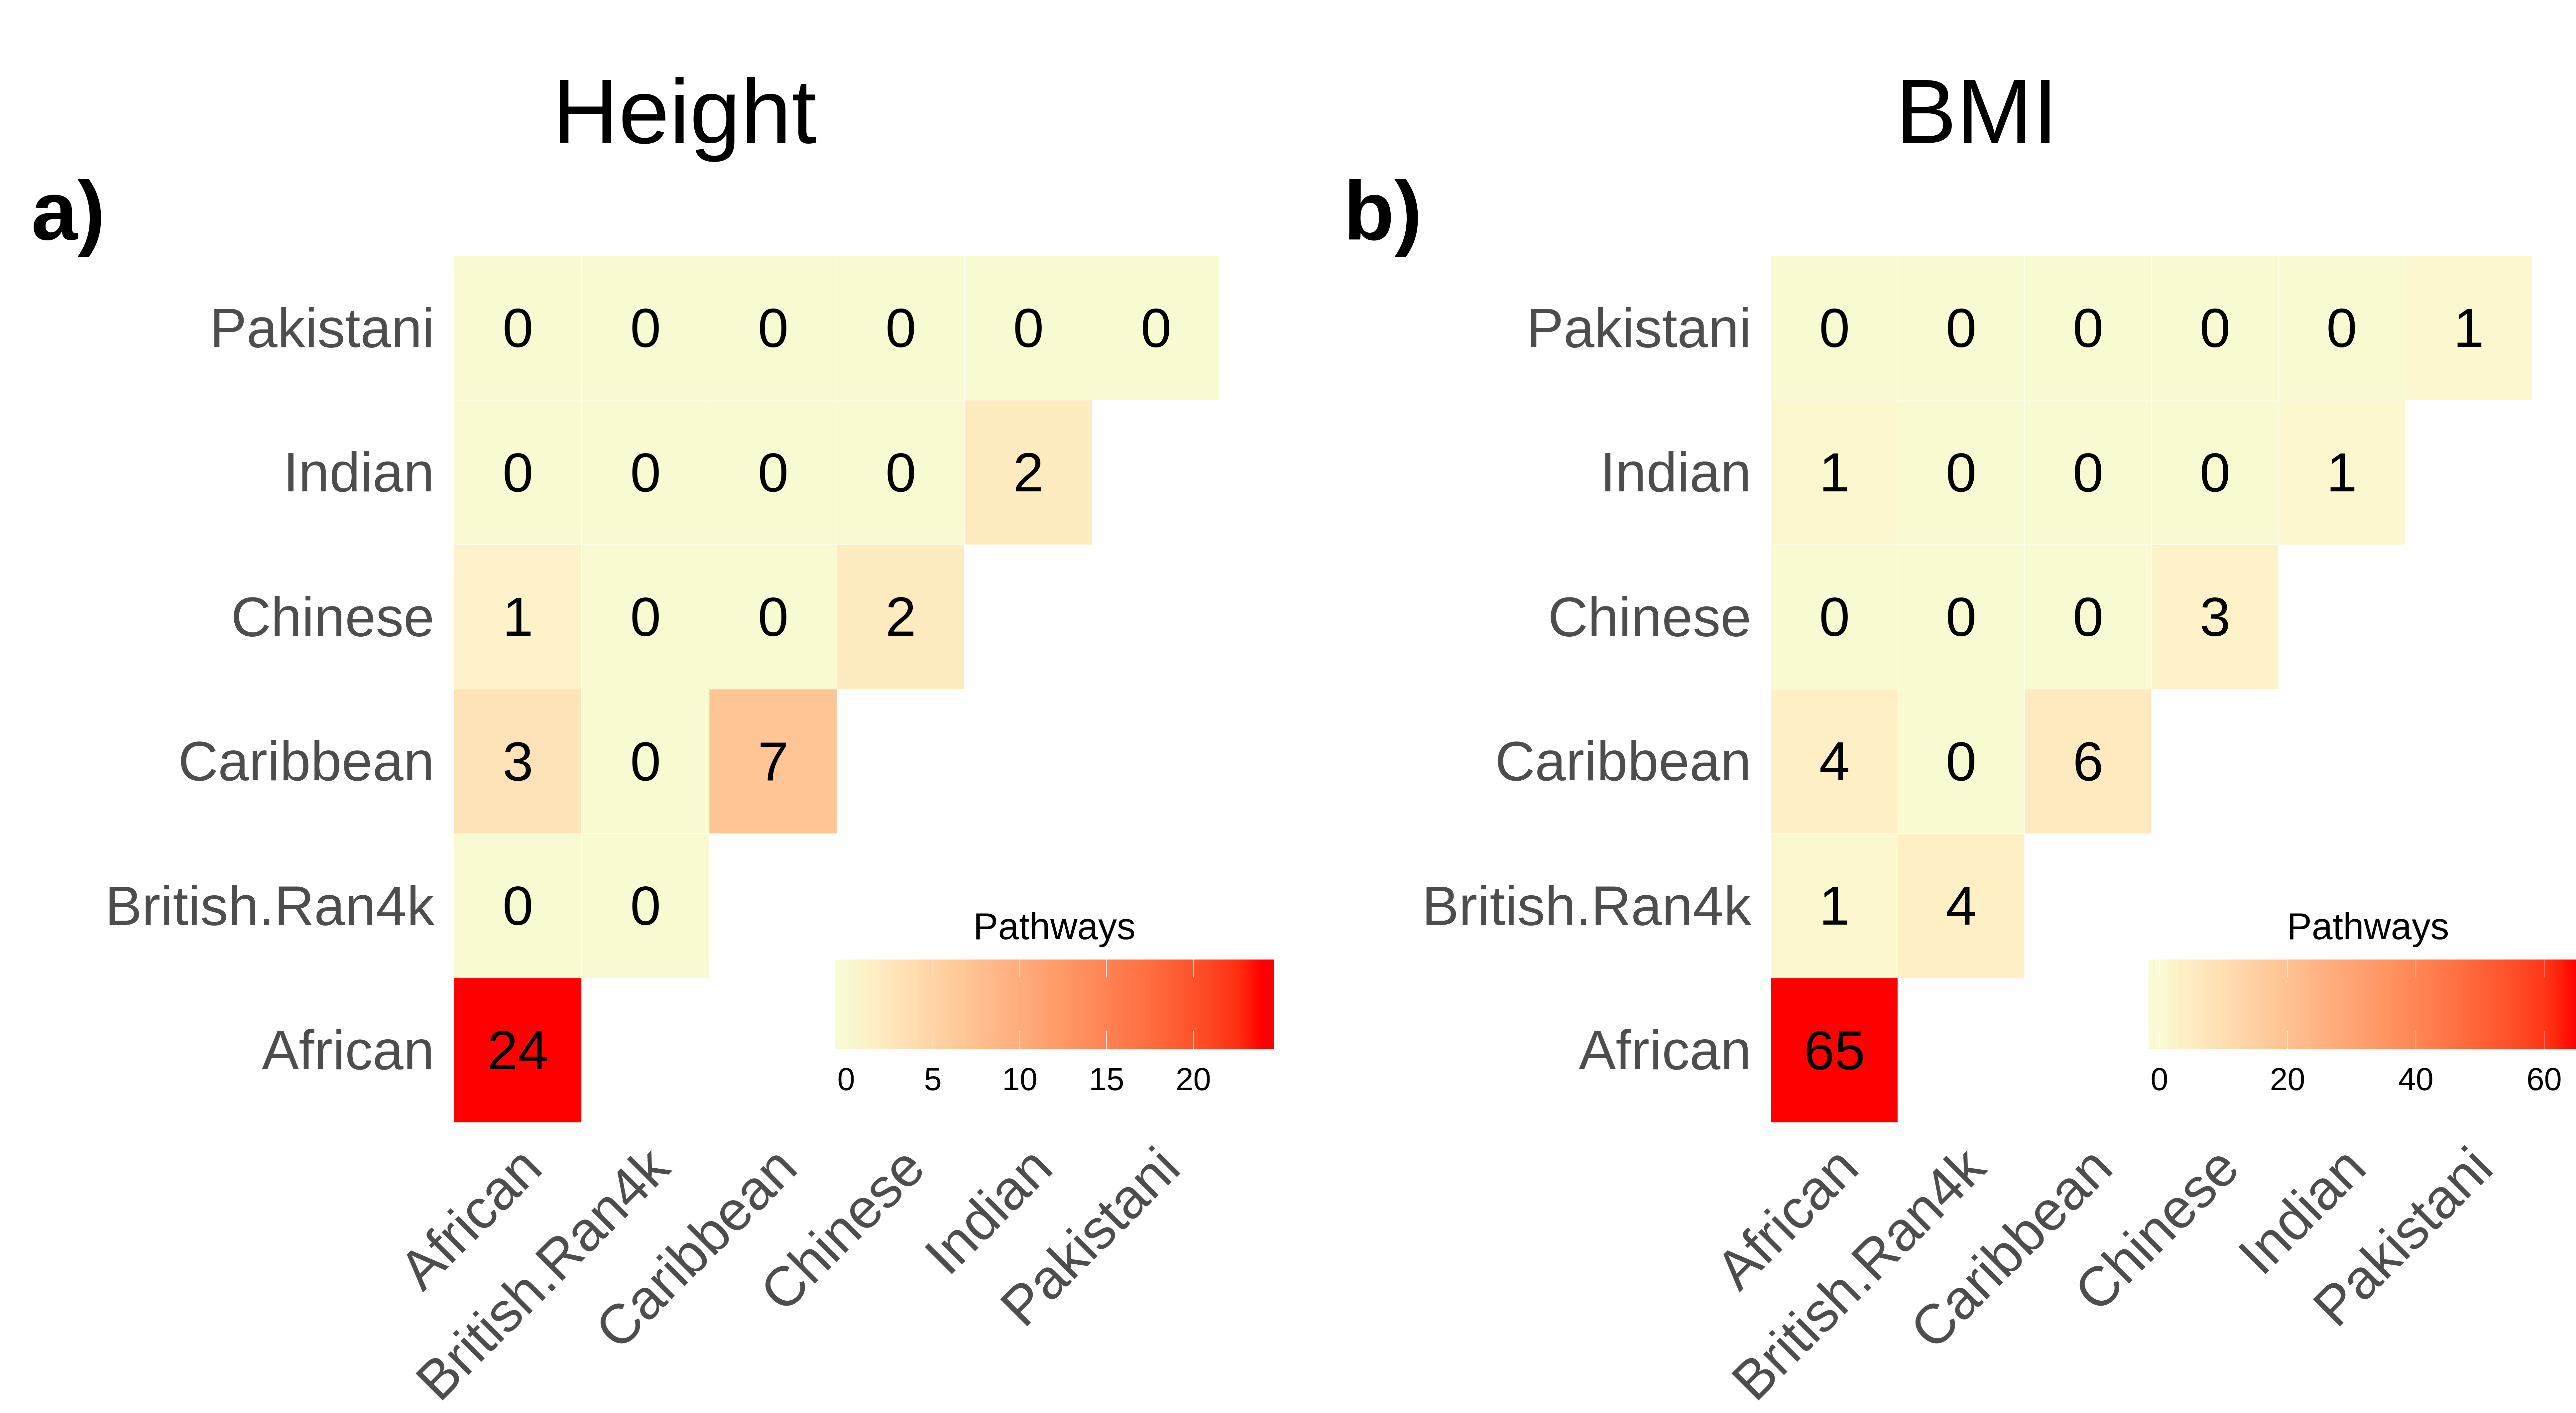
\includegraphics[width = \textwidth]{Images/Supp/InterPath_Supp_Figure_Heatplots_REACTOME_vs4.png}
\caption{\textbf{Heatmaps depicting the overlap of MAPIT-R significant REACTOME pathways for (a) standing height and (b) body mass index (BMI) between the different ancestry-specific subgroups in the UK Biobank}. Here, subgroups in the UK Biobank included individuals based on their self-identified ancestries: ``African'', ``British'', ``Caribbean'', ``Chinese'', ``Indian'', and ``Pakistani'', respectively. Genome-wide significance was determined by using Bonferroni-corrected $P$-value thresholds based on the number of pathways tested in each database-phenotype-subgroup combination (see Supplementary Table \ref{InterPath-Supp-Table-UKBPopStats}). The diagonal shows the total number of genome-wide significant pathways per subgroup. We observe that significant pathways observed in non-African subgroups overlap more often with pathways from the African subgroup than they do with pathways from the other, remaining non-African subgroups. Results for both phenotypes in the KEGG database can be seen in Figure \ref{InterPath-Main-Figure-Heatplots-KEGG} in the main text.}
\label{InterPath-Supp-Figure-Heatplots-REACTOME}
\end{figure}
\clearpage
\setlength{\footskip}{1cm}

\begin{landscape}
\setlength{\footskip}{3cm}
\begin{figure}[htbp]
\centering
\hspace*{-2cm}
\includegraphics[angle=270,scale=.25]{Images/Supp/InterPath_Supp_Figure_MAPITR_PhenoComps_AllPops_vs4.png}
\caption{\textbf{Scatterplots comparing the MAPIT-R $\bm{p}$-values using (top) KEGG and (bottom) REACTOME pathways annotations in height and body mass index (BMI) within all of the different ancestry-specific subgroups in the UK Biobank.} Here, subgroups in the UK Biobank included individuals based on their self-identified ancestries: ``African'', ``British'', ``Caribbean'', ``Chinese'', ``Indian'', and ``Pakistani'', respectively. For each plot, the x-axis depicts the -$\log_{10}$ transformed MAPIT-R $p$-value for height, while the y-axis shows the same results for BMI. The red horizontal and vertical dashed lines are marked at the Bonferroni-corrected $p$-value thresholds for genome-wide significance in each pathway-phenotype combination (see Supplementary Table \ref{InterPath-Supp-Table-UKBPopStats}). Pathways in the top right quadrant have significant marginal epistatic effects in both traits; while, points in the bottom right and top left quadrants are pathways that are uniquely enriched in height or BMI, respectively. Within each plot we also list the Pearson correlation coefficient describing the similarity of marginally epistatic enriched pathways in both traits.}
\label{InterPath-Supp-Figure-MAPITR-PhenoComps-AllPops}
\end{figure}
\clearpage
\setlength{\footskip}{1cm}
\end{landscape}

\begin{figure}[htbp]
\centering
\hspace*{-1.75cm}
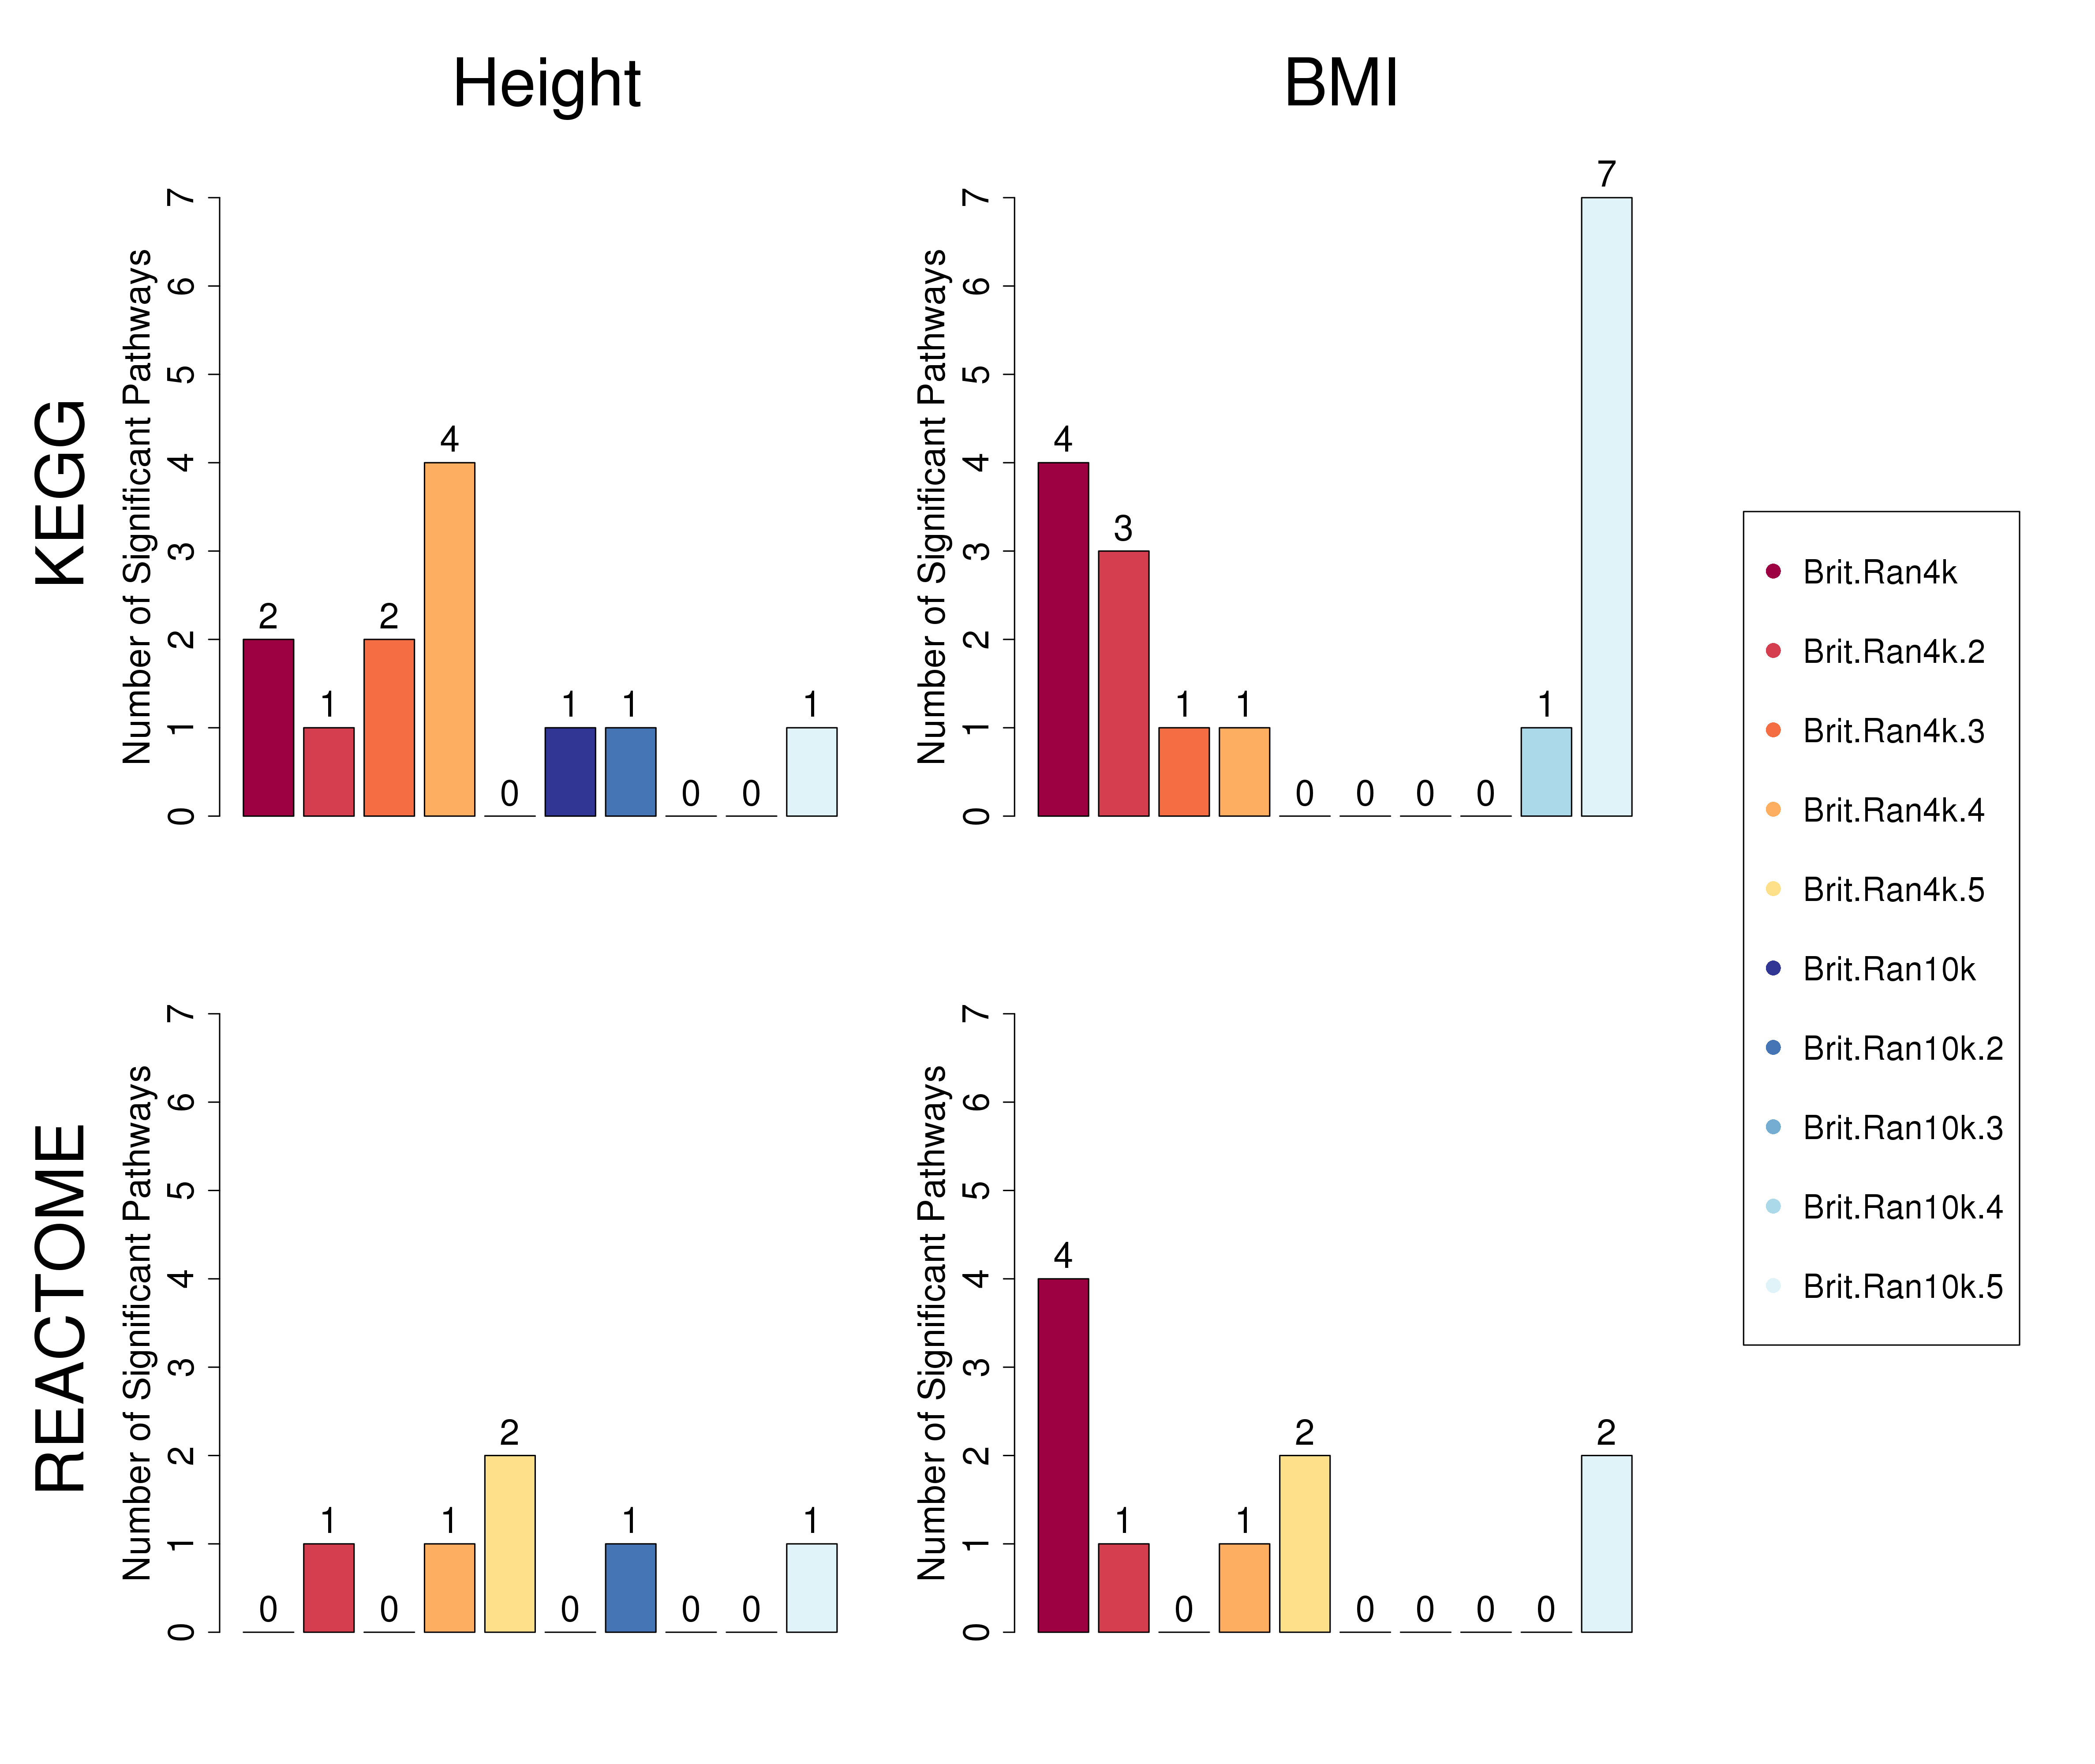
\includegraphics[scale=.45]{Images/Supp/InterPath_Supp_Figure_BritReps_Barplot_vs4.png}
\caption{\textbf{Number of KEGG and REACTOME pathways identified by MAPIT-R that have significant marginal epistatic effects within standing height and body mass index (BMI) per British replicate subgroup in the UK Biobank.} Here, the random subgroups were created by subsampling either $N =$ 4,000 or 10,000 individuals from the full British cohort. In the legend, replicates are marked as numbers after the root tag name (e.g., \texttt{Brit.Ran4k.4} denotes the fourth replicate in the $N =$ 4,000 subsampling scheme). Genome-wide significance was determined by using Bonferroni-corrected $p$-value thresholds based on the number of pathways tested in each database-phenotype-subgroup combination (see Supplementary Table \ref{InterPath-Supp-Table-UKBPopStats}). Note that most replicate runs did not produce many significant results.}
\label{InterPath-Supp-Figure-BritReps-Barplots}
\end{figure}
\clearpage

%\newcounter{CharNumber4}
%\setcounter{CharNumber4}{1}
%\renewcommand{\thefigure}{\arabic{figure}\alph{CharNumber4}}
\begin{landscape}
\begin{figure}[htbp]
\centering
\includegraphics[scale=.2]{Images/Supp/InterPath_Supp_Figure_BritReps_Heatplots_KEGG_vs4.png}
\caption{\textbf{Heatmaps depicting the overlap of MAPIT-R significant KEGG pathways for (a) standing height and (b) body mass index (BMI) per British replicate subgroup in the UK Biobank}. Here, the random subgroups were created by subsampling either $N =$ 4,000 or 10,000 individuals from the full British cohort. In the legend, replicates are marked as numbers after the root tag name (e.g., \texttt{Brit.Ran4k.4} denotes the fourth replicate in the $N =$ 4,000 subsampling scheme). Genome-wide significance was determined by using Bonferroni-corrected $P$-value thresholds based on the number of pathways tested in each database-phenotype-subgroup combination (see Supplementary Table \ref{InterPath-Supp-Table-UKBPopStats}). The diagonal shows the total number of genome-wide significant pathways per subgroup. We do not observe much overlap between enriched pathways between the replicate subgroups --- even though they all consist of individuals of the same ancestry.}
\label{InterPath-Supp-Figure-BritReps-Heatplots-AllPaths-KEGG}
\end{figure}
\clearpage
%\addtocounter{figure}{-1}
%\addtocounter{CharNumber4}{1}
\end{landscape}

\begin{landscape}
\begin{figure}[htbp]
\centering
\includegraphics[scale=.2]{Images/Supp/InterPath_Supp_Figure_BritReps_Heatplots_REACTOME_vs4.png}
\caption{\textbf{Heatmaps depicting the overlap of MAPIT-R significant REACTOME pathways for (a) standing height and (b) body mass index (BMI) per British replicate subgroup in the UK Biobank}. Here, the random subgroups were created by subsampling either $N =$ 4,000 or 10,000 individuals from the full British cohort. In the legend, replicates are marked as numbers after the root tag name (e.g., \texttt{Brit.Ran4k.4} denotes the fourth replicate in the $N =$ 4,000 subsampling scheme). Genome-wide significance was determined by using Bonferroni-corrected $P$-value thresholds based on the number of pathways tested in each database-phenotype-subgroup combination (see Supplementary Table \ref{InterPath-Supp-Table-UKBPopStats}). The diagonal shows the total number of genome-wide significant pathways per subgroup. We do not observe much overlap between enriched pathways between the replicate subgroups --- even though they all consist of individuals of the same ancestry.}
\label{InterPath-Supp-Figure-BritReps-Heatplots-AllPaths-REACTOME}
\end{figure}
\clearpage
\end{landscape}
%\renewcommand{\thefigure}{\arabic{figure}}

\begin{figure}[htbp]
\centering
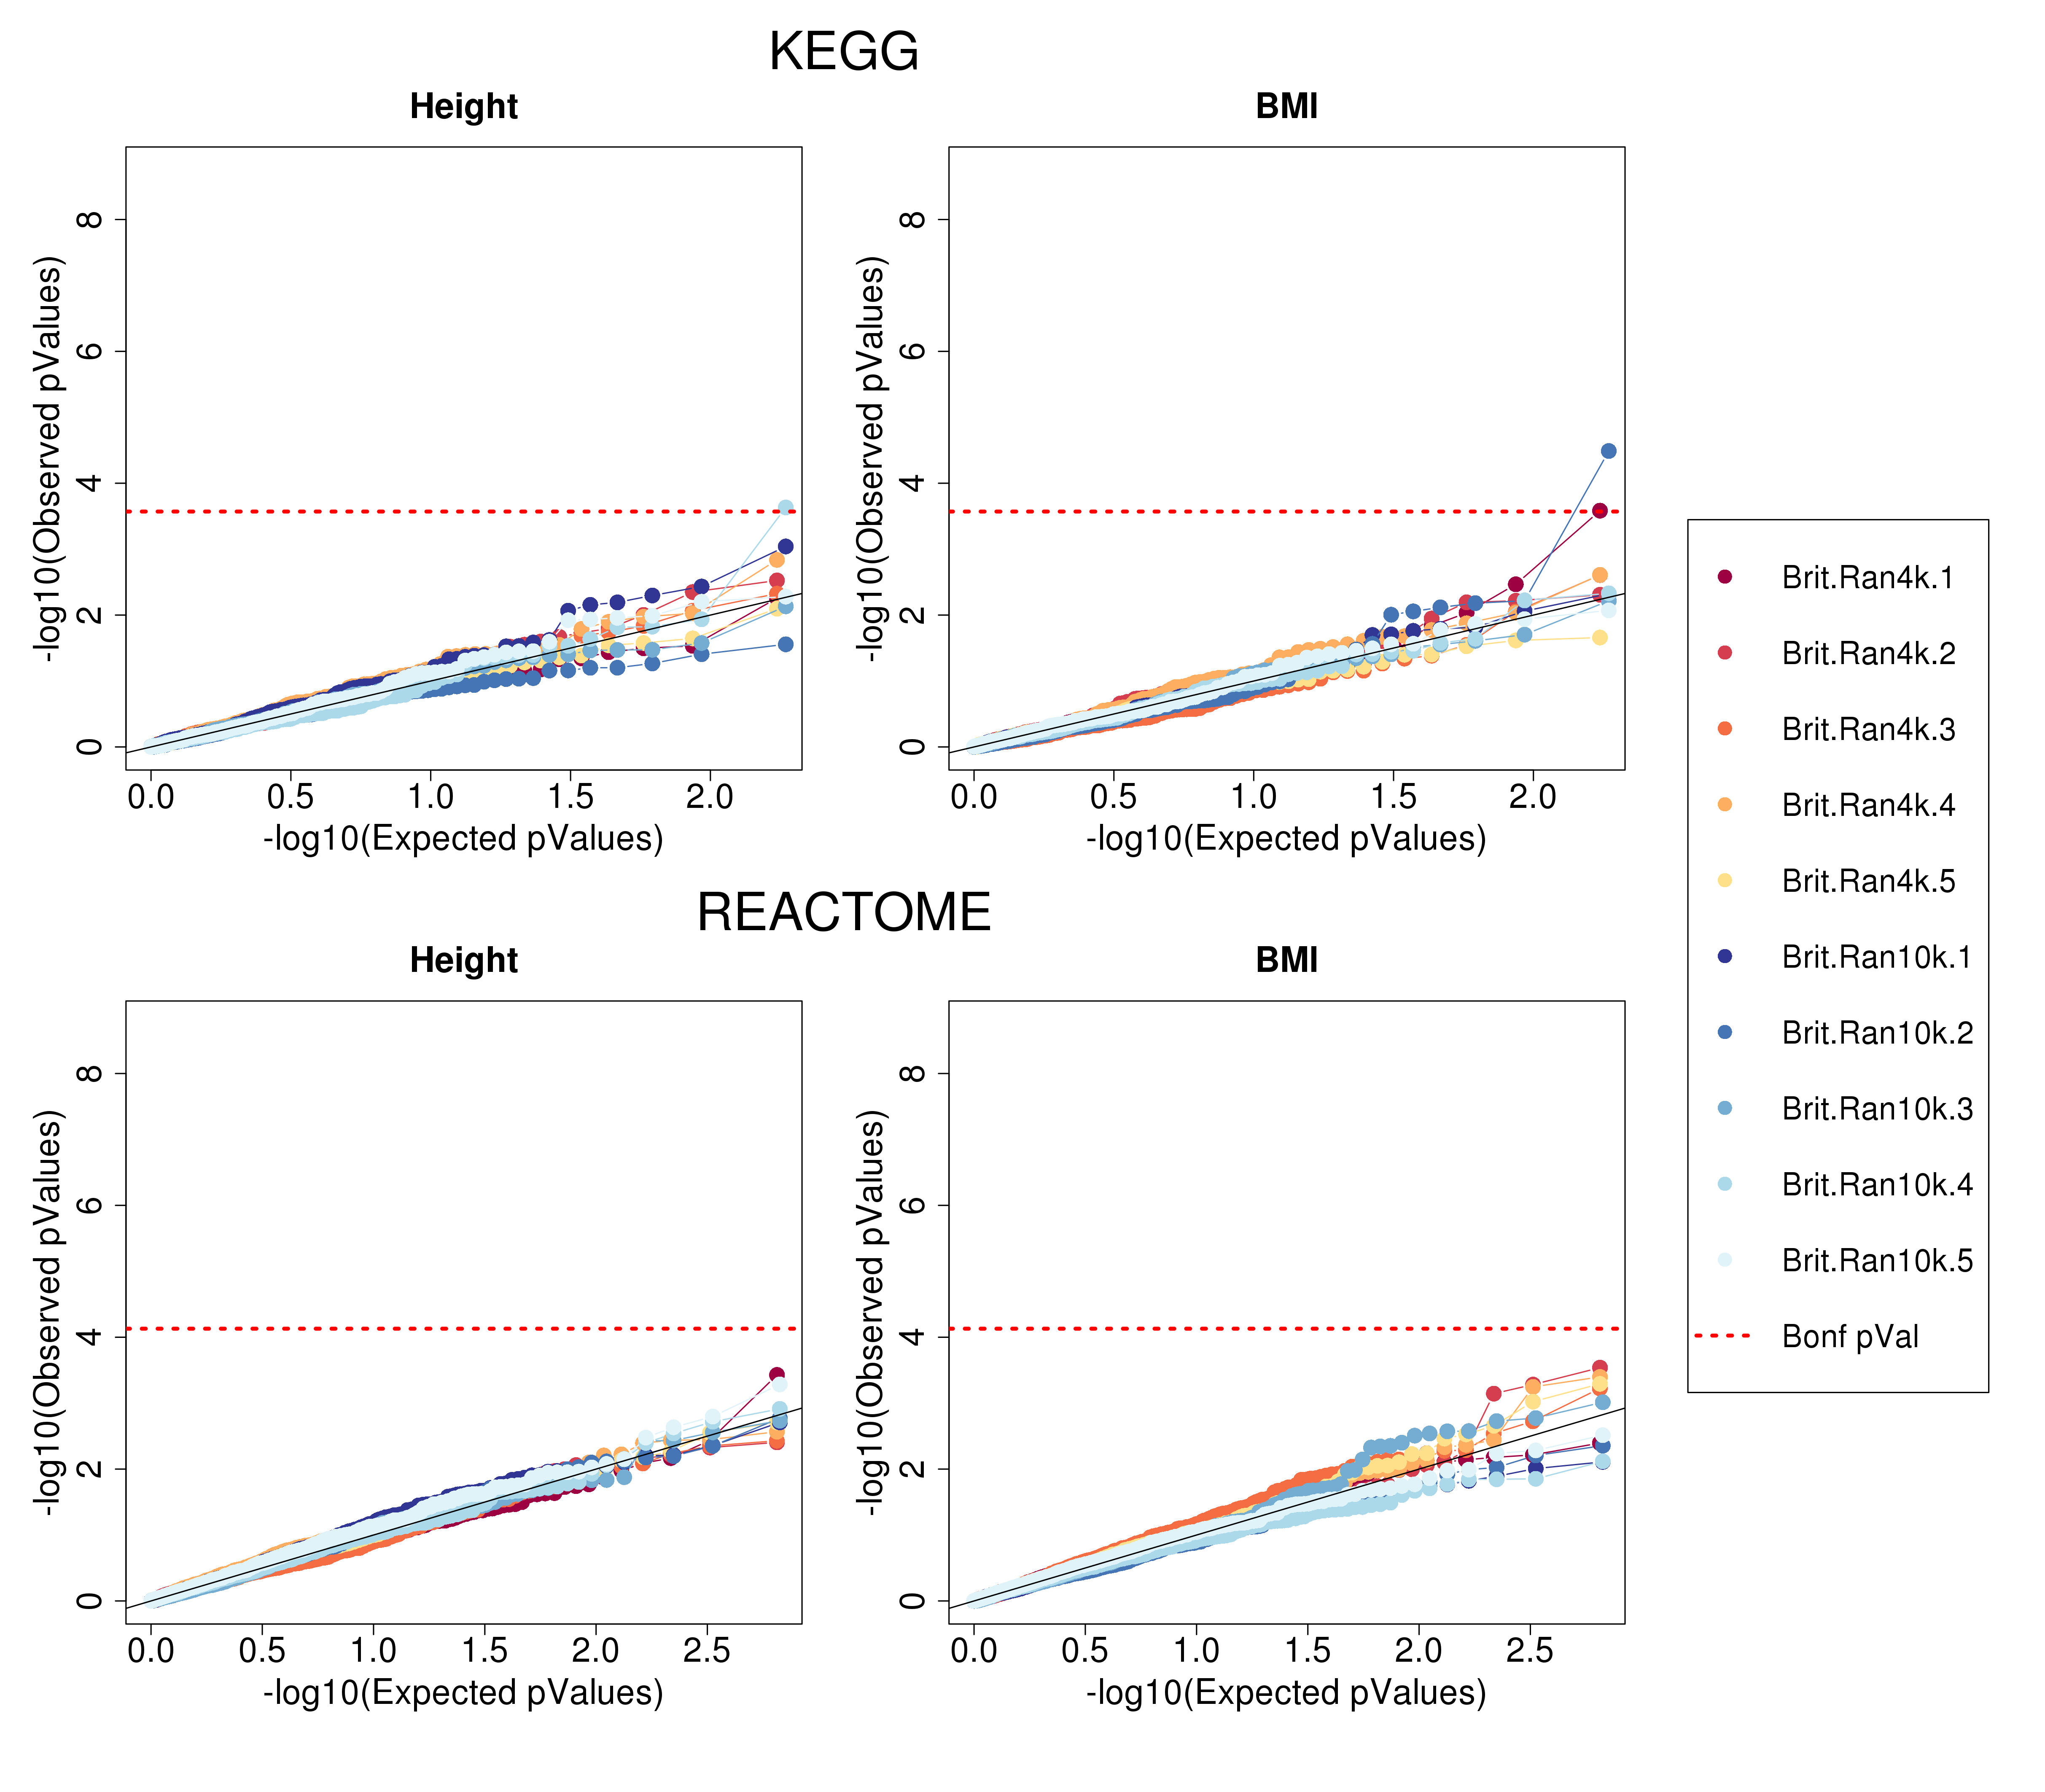
\includegraphics[width=\textwidth]{Images/Supp/InterPath_Supp_Figure_BritReps_perm1_QQPlots_AllPaths_vs1.png}
\caption{\textbf{QQ-Plots of MAPIT-R $\bm{p}$-values using KEGG and REACTOME pathways annotations and randomly permuted phenotypes in British replicate subgroups from the UK Biobank.} Here, we run MAPIT-R after conducting a single random permutation of either height or BMI measurements. Note that traits were permuted within each population subgroup ten different times. Shown on the x-axis are the -$\log_{10}$ transformed expected $p$-values, while the $y$-axis shows the -$\log_{10}$ observed $p$-values. The random subgroups were created by subsampling either $N =$ 4,000 or 10,000 individuals from the full British cohort. In the legend, replicates are marked as numbers after the root tag name (e.g., \texttt{Brit.Ran4k.4} denotes the fourth replicate in the $N =$ 4,000 subsampling scheme). The dotted red line is the Bonferroni-corrected $P$-value threshold based on the number of pathways tested per database-phenotype combination (Supplementary Table \ref{InterPath-Supp-Table-UKBPopStats}). Overall, we find that MAPIT-R continues to exhibit well-calibrated behavior under the null hypothesis and properly controls for type 1 error rate.}
\label{InterPath-Supp-Figure-BritReps-perm1-QQPlots-AllPaths}
\end{figure}
\clearpage

%\newcounter{CharNumber3}
%\setcounter{CharNumber3}{1}
%\renewcommand{\thefigure}{\arabic{figure}\alph{CharNumber3}}
\setlength{\footskip}{1cm}
\begin{figure}[htbp]
\centering
%\vspace*{-1cm}
\includegraphics[width=\textwidth]{Images/Supp/InterPath_Supp_Figure_BritReps_pValHists_AllPaths_vs1_pt1.png}
\caption{\textbf{Histograms of MAPIT-R $\bm{p}$-values using KEGG and REACTOME pathways annotations and randomly permuted phenotypes in each \textcolor{red}{British 4,000 replicate} subgroup in the UK Biobank.} Here, we run MAPIT-R after conducting a single random permutation of either height or BMI measurements. Note that traits were independently permuted within each population subgroup ten different times. The random subgroups were created by subsampling $N =$ 4,000 individuals from the full British cohort. In the legend, replicates are marked as numbers after the root tag name (e.g., \texttt{Brit.Ran4k.4} denotes the fourth replicate in the $N =$ 4,000 subsampling scheme). Overall, we find that MAPIT-R continues to exhibit well-calibrated behavior under the null hypothesis.}
\label{InterPath-Supp-Figure-BritReps-10perms-pValHists-pt1}
\end{figure}
\clearpage
\setlength{\footskip}{1cm}
%\addtocounter{figure}{-1}
%\addtocounter{CharNumber3}{1}

\setlength{\footskip}{2cm}
\begin{figure}[htbp]
\centering
%\vspace*{-1cm}
\includegraphics[width=\textwidth]{Images/Supp/InterPath_Supp_Figure_BritReps_pValHists_AllPaths_vs1_pt2.png}
\caption{\textbf{Histograms of MAPIT-R $\bm{P}$-values using KEGG and REACTOME pathways annotations and randomly permuted phenotypes in each \textcolor{red}{British 10,000 replicate} subgroup in the UK Biobank.} Here, we run MAPIT-R after conducting a single random permutation of either height or BMI measurements. Note that traits were independently permuted within each population subgroup ten different times. The random subgroups were created by subsampling $N =$ 10,000 individuals from the full British cohort. In the legend, replicates are marked as numbers after the root tag name (e.g., \texttt{Brit.Ran10k.4} denotes the fourth replicate in the $N =$ 10,000 subsampling scheme). Overall, we find that MAPIT-R continues to exhibit well-calibrated behavior under the null hypothesis.}
\label{InterPath-Supp-Figure-BritReps-10perms-pValHists-pt2}
\end{figure}
\clearpage
\setlength{\footskip}{1cm}
%\renewcommand{\thefigure}{\arabic{figure}}

\setlength{\footskip}{3cm}
\begin{figure}[htbp]
\centering
\vspace*{-2cm}
\includegraphics[scale=.2]{Images/Supp/InterPath_Supp_Figure_pValsVsNumSNPs_vs3.png}
\caption[TBD]{\textbf{Number of SNPs in a pathway versus a pathway's MAPIT-R $p$-value}. Caption continued on next page.}
\label{InterPath-Supp-Figure-pValsVsNumSNPs}
\end{figure}
\clearpage
\setlength{\footskip}{1cm}

\addtocounter{figure}{-1}
\begin{figure} [t!]
  \caption{\textbf{Number of SNPs in a pathway versus a pathway's MAPIT-R $p$-value}. The figure shows plots comparing the MAPIT-R $p$-values from our main analysis to the number of SNPs present in each pathway. Results for every pathway database-phenotype-UB subgroup combinations are shown. The dotted red line is the line of best fit and the legend provides the regression coefficient and its associated $p$-value. We observe that for most combinations there is a significant relationship between MAPIT-R $p$-value and the number of SNPs present in a pathway. This follows our hypothesis that combining SNPs together in a joint analysis might provide greater power to detect marginal epistasis than analyzing each SNP independently. We note, however, that these results appear to not solely be driven just by the presence or absence of large SNP counts -- conducting this same analysis on one of our sets of permuted phenotypes we now find very few significant relationships between MAPIT-R $p$-values and pathway SNP counts (Supplementary Figure \ref{InterPath-Supp-Figure-pValsVsNumSNPs-perm1}).}
\label{InterPath-Supp-Figure-pValsVsNumSNPs-Caption}
\end{figure}
\clearpage

\setlength{\footskip}{3cm}
\begin{figure}[htbp]
\centering
\vspace*{-2cm}
\includegraphics[scale=.2]{Images/Supp/InterPath_Supp_Figure_pValsVsNumSNPs_perm1_vs3.png}
\caption[TBD]{\textbf{Number of SNPs in a pathway versus a pathway's MAPIT-R $p$-value using permuted phenotypes}. Caption continued on next page.}
\label{InterPath-Supp-Figure-pValsVsNumSNPs-perm1}
\end{figure}
\clearpage
\setlength{\footskip}{1cm}

\addtocounter{figure}{-1}
\begin{figure} [t!]
  \caption{\textbf{Number of SNPs in a pathway versus a pathway's MAPIT-R $p$-value using permuted phenotypes}. The figure shows plots comparing the MAPIT-R $p$-values from our main analysis to the number of SNPs present in each pathway. For this analysis a single set of our permuted phenotypes (i.e. Supplementary Figure \ref{InterPath-Supp-Figure-perm1-QQPlots-AllPaths}) was used for each UKB subgroup. Results for every pathway database-phenotype-subgroup combination is shown. The dotted red line is the line of best fit and the legend provides the regression coefficient and its associated $p$-value. We observe that for very few combinations there is any relationship between MAPIT-R $p$-value and the number of SNPs present in a pathway. For the same analysis on the original set of observed phenotypes, see Supplementary Figure \ref{InterPath-Supp-Figure-pValsVsNumSNPs}.}
\label{InterPath-Supp-Figure-pValsVsNumSNPs-perm1-Caption}
\end{figure}
\clearpage

%\begin{figure}[htb]
%\centering
%\hspace*{-1.4cm}
%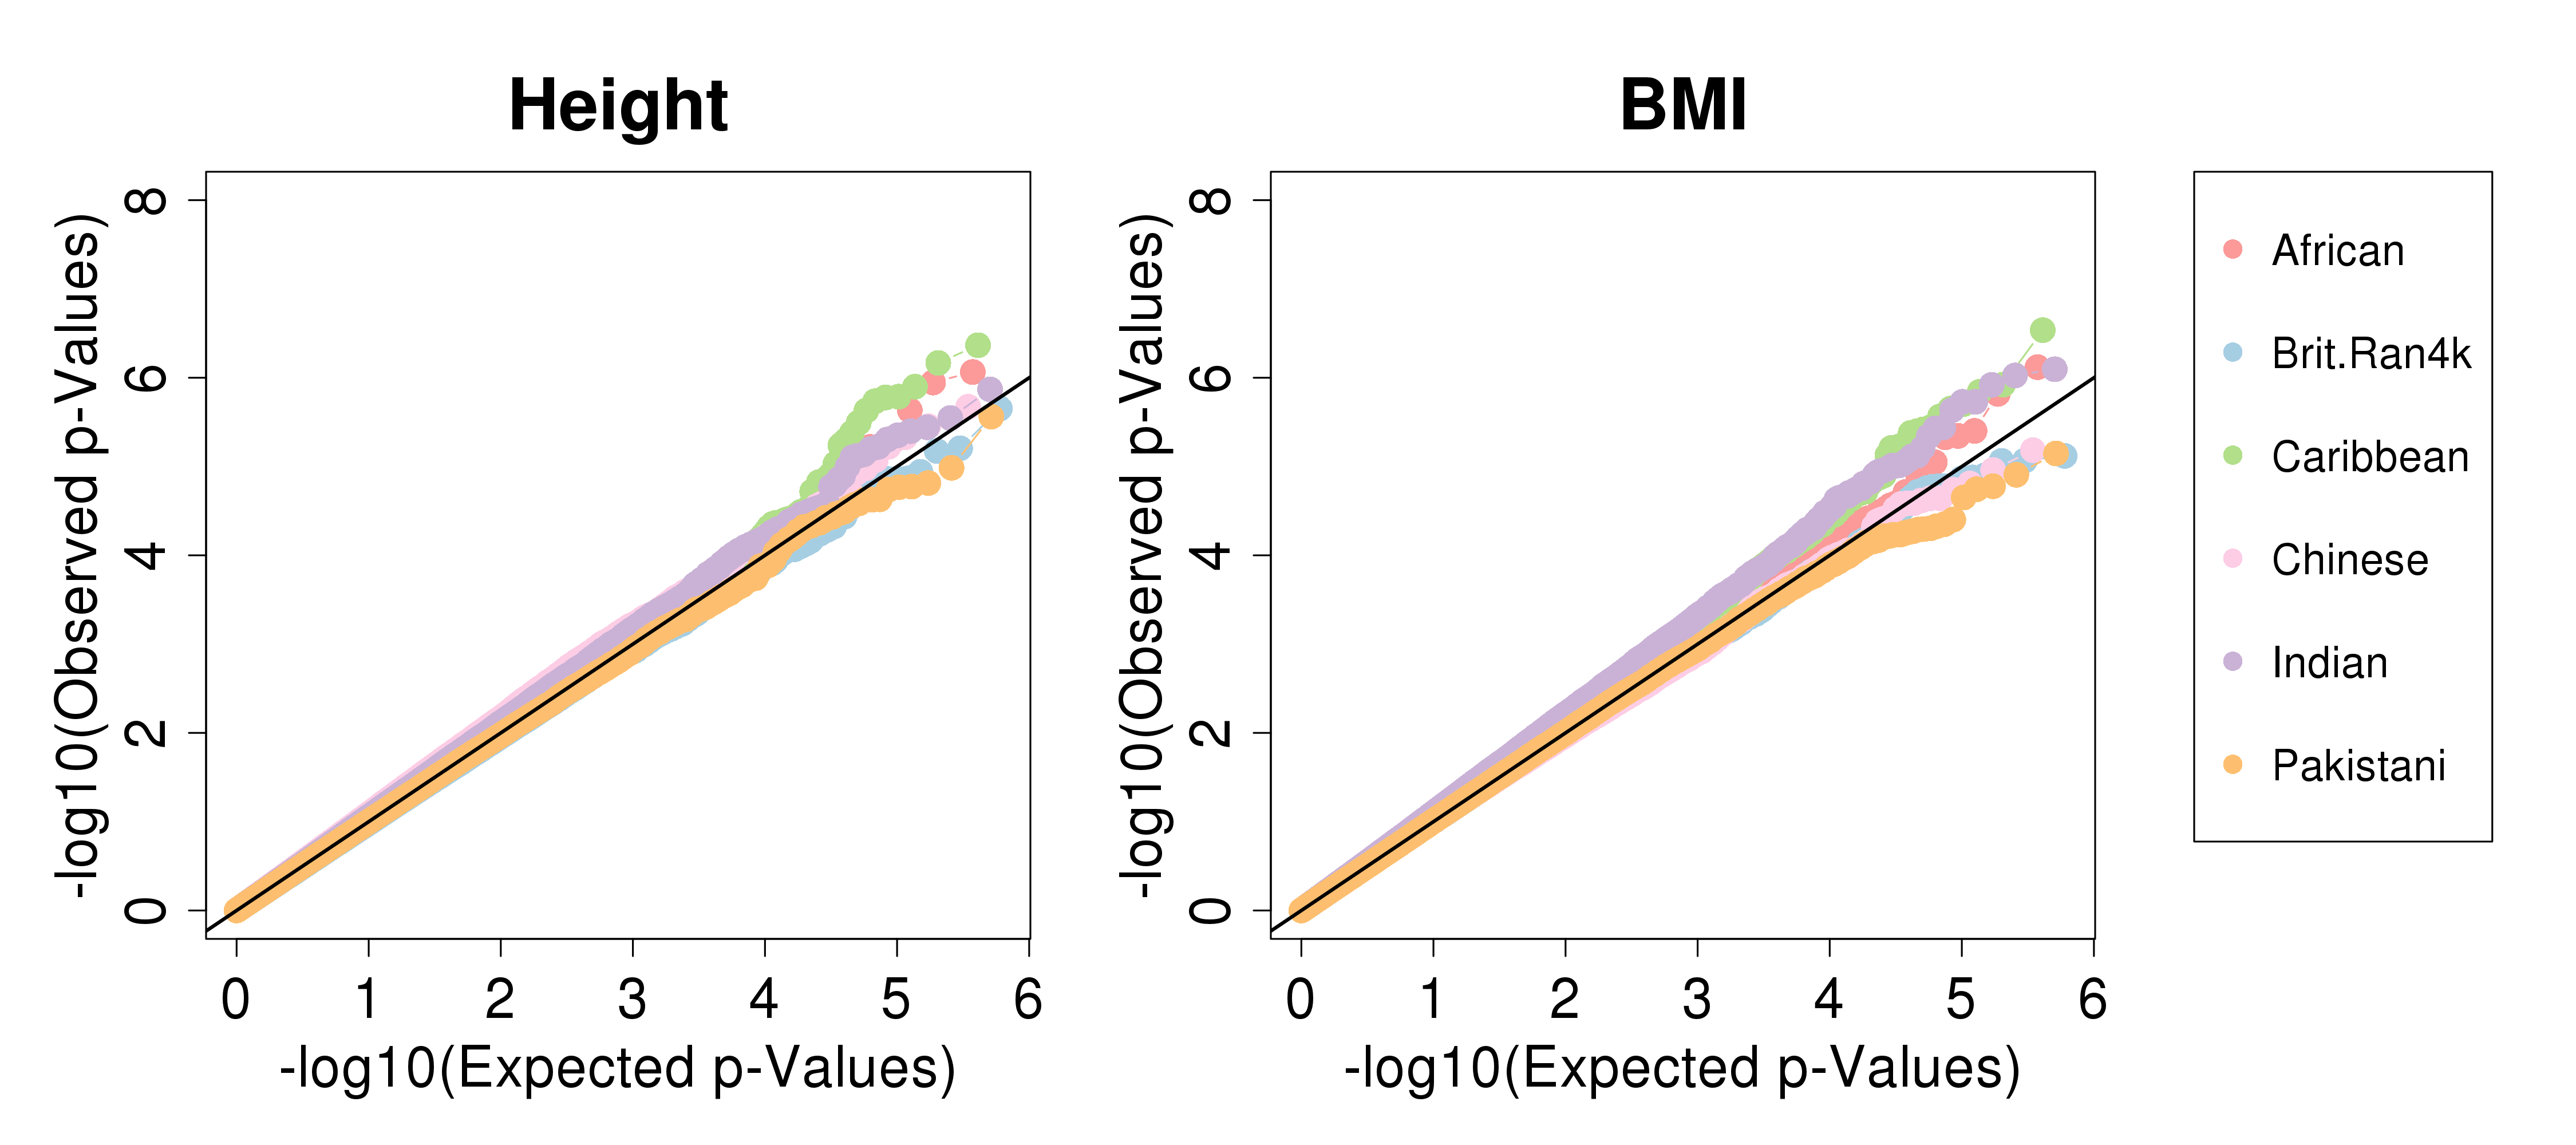
\includegraphics[scale=.45]{Images/Main/InterPath_Main_Figure_MAPIT_vs4_HeightBMI.png}
%\caption[TBD]{\textbf{QQ-Plots of MAPIT results, per subgroup}. The figure shows QQ-plots of our results from running MAPIT on our four initial UKB population subgroups in height and BMI. On the $x$-axis are the -$\log_{10}$ of the expected $p$-values and the on the $y$-axis are on the -$\log_{10}$ of the observed $p$-values. Each data point is a SNP and total SNP counts per UKB subgroup can be found in Supplementary Table \ref{InterPath-Supp-Table-UKBPopStats}. We observe no genome-wide significant signals in any subgroup across both phenotypes ($p$-value $< 5\times10^{-8}$) and, due to this lack of significant results, observe no clear differences in patterns between our subgroups.}
%\label{InterPath-Supp-Figure-MAPIT-HeightBMI}
%\end{figure}

%\begin{figure}[htbp]
%\centering
%\hspace*{-1.7cm}
%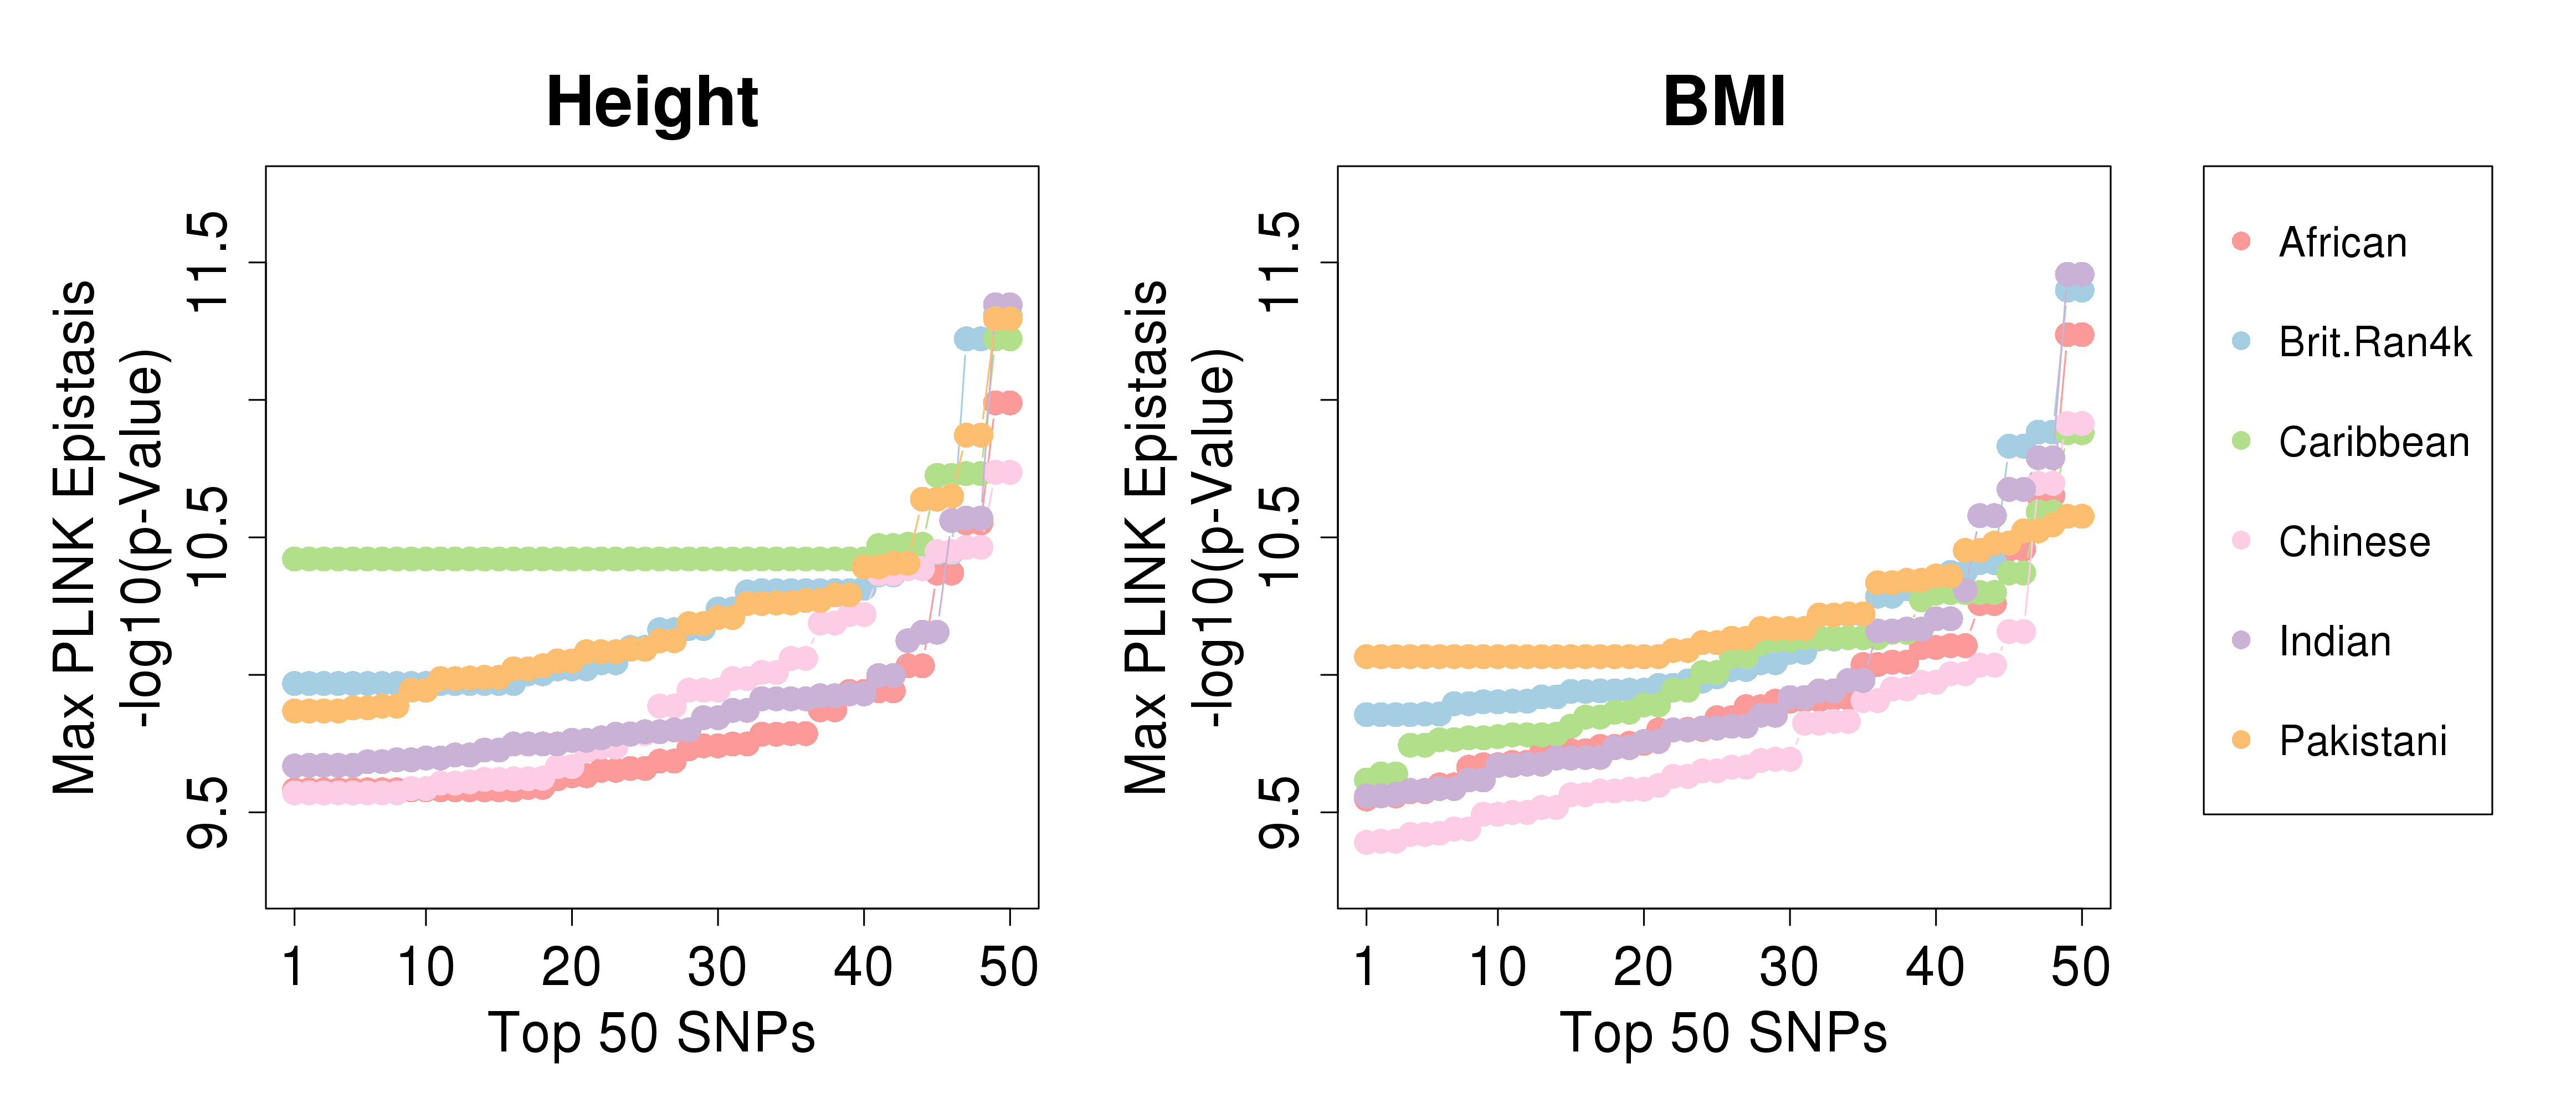
\includegraphics[scale=.45]{Images/Supp/InterPath_Supp_Figure_PLINK_BestSNPs_vs2_AllPops_HeightBMI.png}
%\caption[TBD]{\textbf{SNPs with the largest PLINK pairwise epistasis signals, per subgroup}. The figure shows the best $p$-values obtained from running PLINK's exhaustive pairwise SNP epistasis test for both height and BMI in each of the UKB subgroups. Only the top 50 SNPs, sorted by best pairwise SNP epistasis $p$-value, for each subgroup are shown. No test reaches genome-wide significance based on using a Bonferroni-corrected $p$-value threshold ($p$-value $< 5\times10^{-13}$).}
%\label{InterPath-Supp-Figure-PLINK-HeightBMI-AllPops}
%\end{figure}
%\clearpage

%From: ,https://tex.stackexchange.com/questions/64934/subfig-label-positioning, https://tex.stackexchange.com/questions/196653/how-do-i-stack-two-figures-on-top-of-each-other-rather-than-side-to-side, https://tex.stackexchange.com/questions/47311/include-table-as-a-subfigure, https://tex.stackexchange.com/questions/169541/looking-for-three-images-on-top-of-each-other-with-text-underneath-each, https://tex.stackexchange.com/questions/10863/is-there-a-way-to-slightly-shrink-a-table-including-font-size-to-fit-within-th

\newcounter{CharNumber5}
\setcounter{CharNumber5}{1}
\renewcommand{\thefigure}{\arabic{figure}\alph{CharNumber5}}
\begin{figure}[ht]
\centering
\vspace*{-.5cm}
\subfloat[]{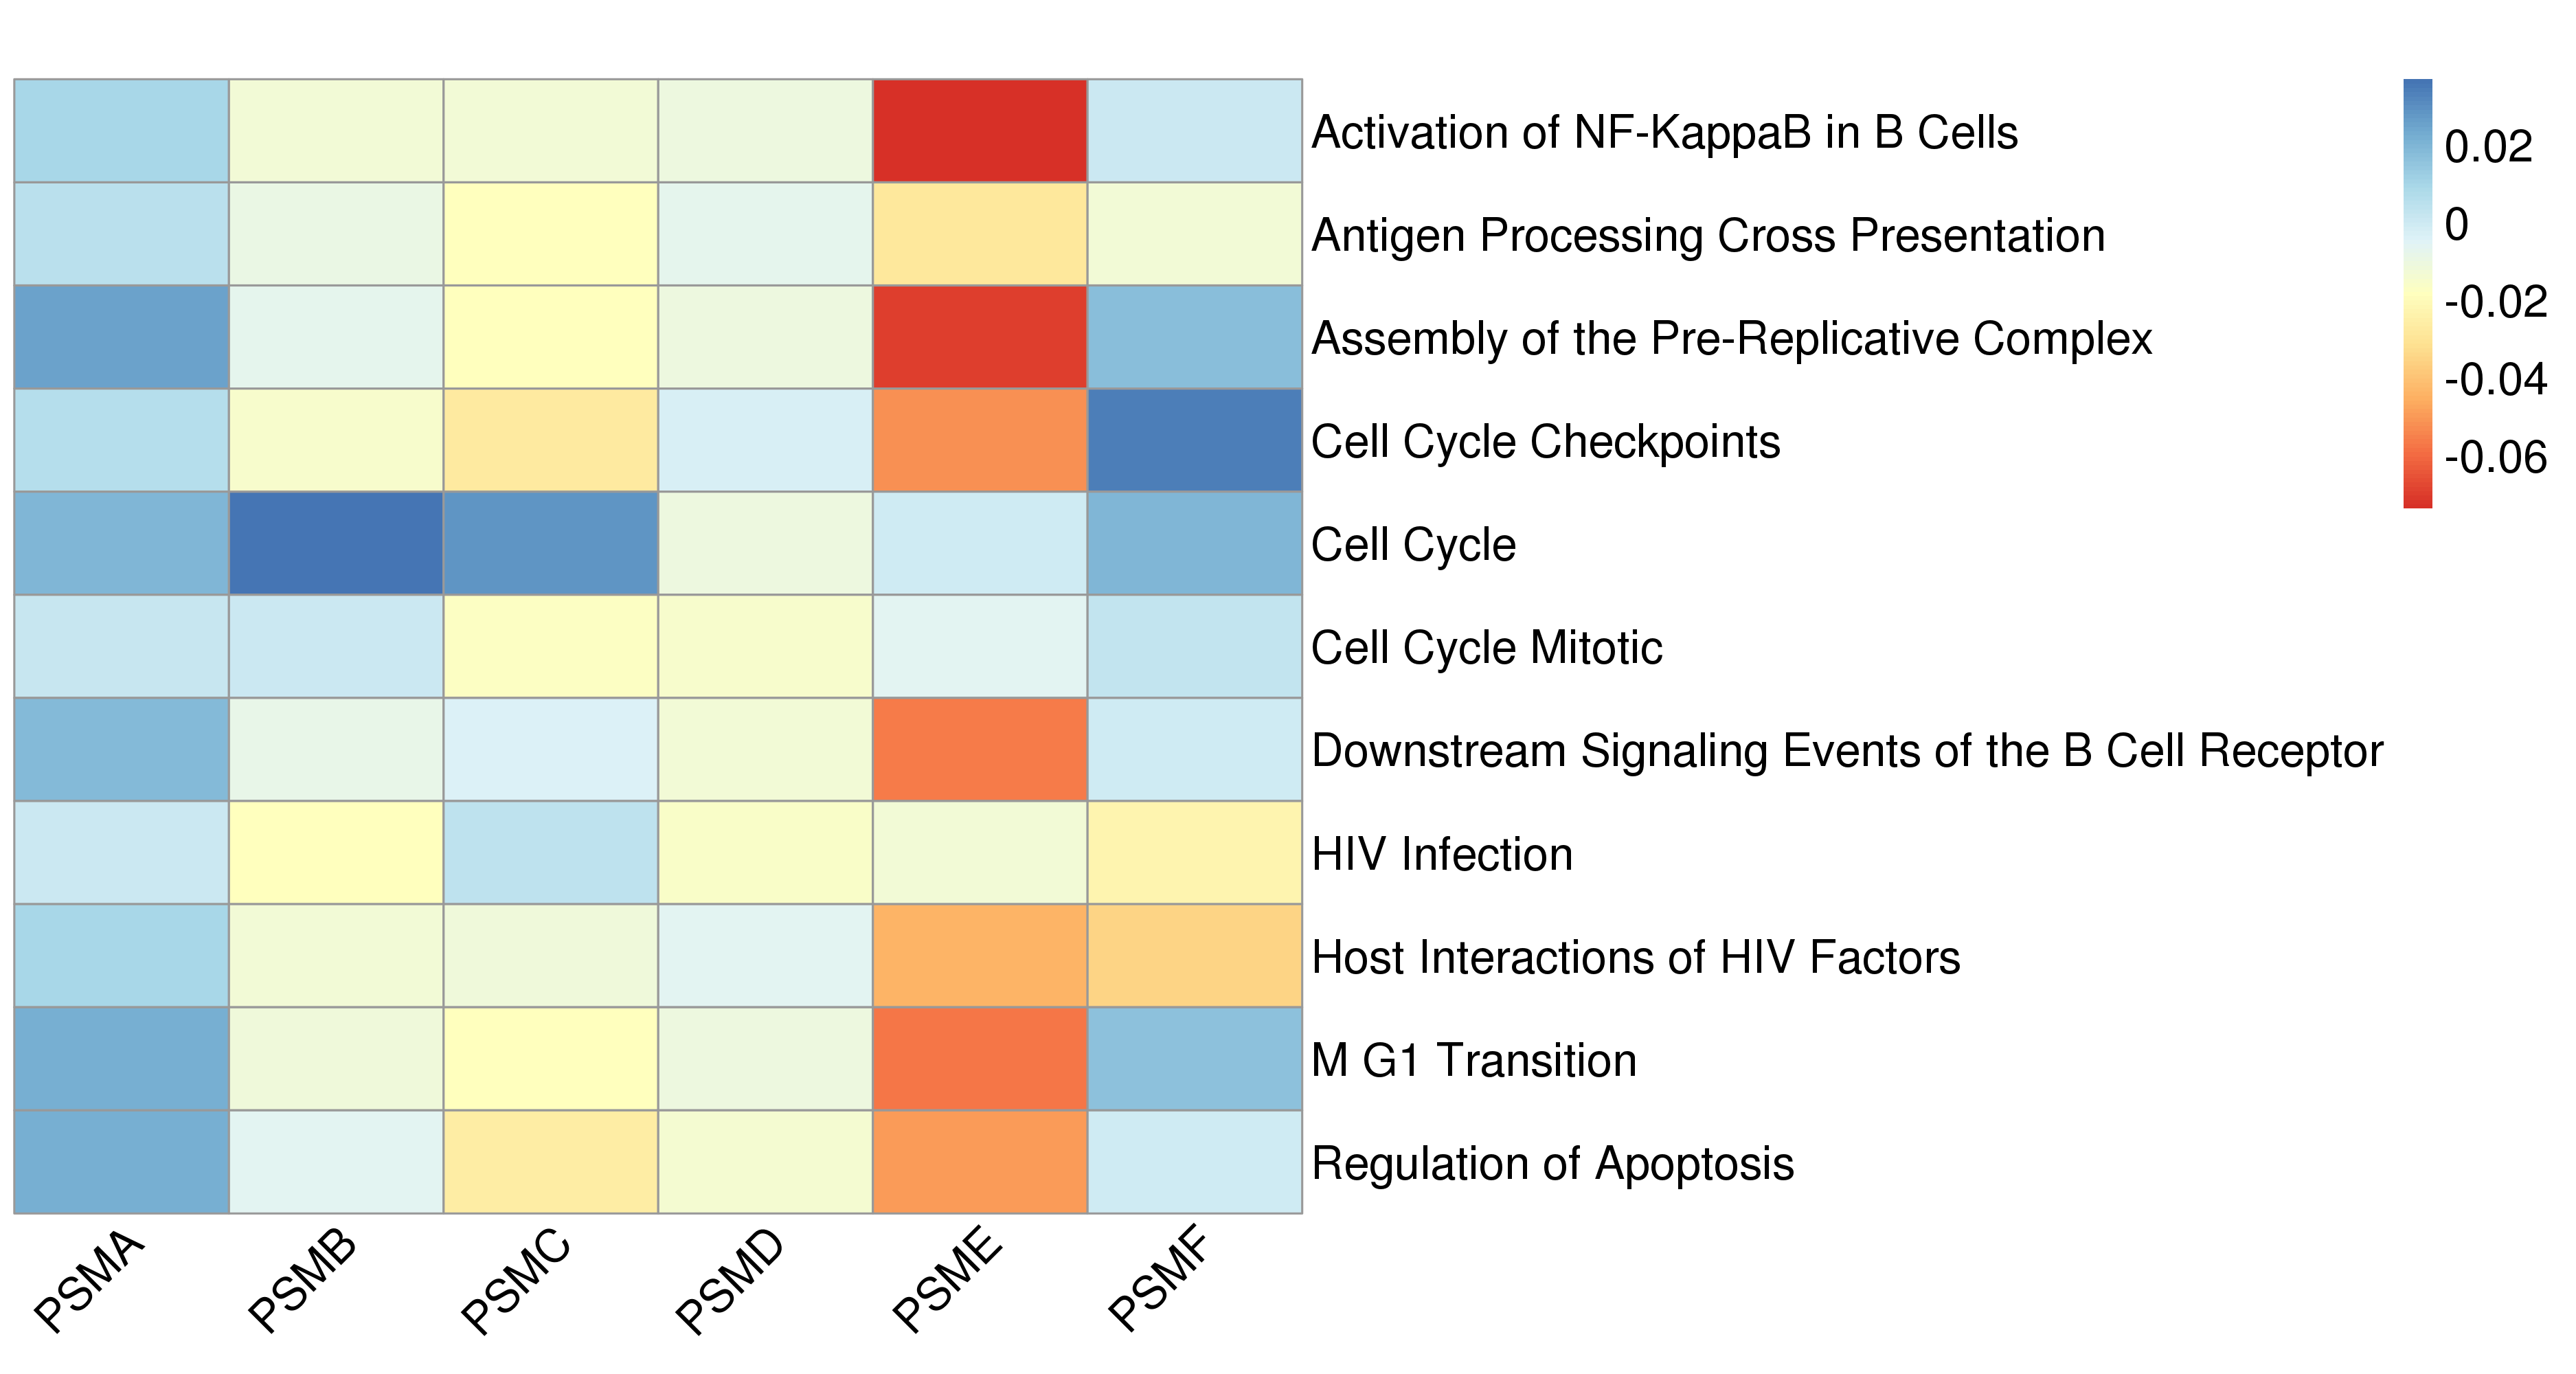
\includegraphics[scale=.5]{Images/Supp/InterPath_Supp_Figure_Proteaseome_Heatplots_African_Loop_vs3.png}}
\par
\subfloat[]{\resizebox{1.1\columnwidth}{!}{
 \hspace*{-1.75cm}
 \begin{tabular}{cc|ccc}
  \hline
\textbf{Proteasome} & \textbf{SNPs} & \textbf{REACTOME} & \textbf{SNPs} & \textbf{MAPIT-R} \\
 \textbf{Gene Family} & & \textbf{Pathway} & & \textbf{$p$-Value} \\
  \hline
PSMA & 17 & Activation of NF-KappaB in B Cells & 465 & 1.86E-05  \\
PSMB & 74 & Antigen Processing Cross Presentation & 850 & 3.96E-05 \\
PSMC & 20 & Assembly of the Pre-Replicative Complex & 331 & 3.29E-05 \\
PSMD & 62 & Cell Cycle Checkpoints & 670 & 5.78E-06 \\
PSME & 15 & Cell Cycle & 2459 & 1.29E-06 \\
PSMF & 16 & Cell Cycle Mitotic & 1906 & 4.51E-05 \\
 & & Downstream Signaling Events of the B Cell Receptor & 745 & 1.19E-05 \\
 & & HIV Infection & 1346 & 7.53E-07 \\
 & & Host Interactions of HIV Factors & 963 & 7.52E-06 \\
 & & M G1 Transition & 458 & 3.19E-06 \\
 & & Regulation of Apoptosis & 564 & 1.22E-05 \\
  \hline
\end{tabular}}}
\caption[TBD]{\textbf{Proteasome gene family leave-one-out MAPIT-R reruns, REACTOME-BMI-African}. (a) The figure shows the change in original MAPIT-R -$\log_{10}$ $p$-value for each presented REACTOME pathway when each proteasome gene family is removed one at a time. The analyses were conducted in the BMI-African subgroup combination. The $x$-axis shows each proteasome gene family and the $y$-axis shows each REACTOME pathway. Each column has been scaled by the number of SNPs present in the given gene family and, as a result, the heatplot specifically shows the -$\log_{10}$ $p$-value change per SNP. (b) The table shows the number of SNPs that are present in each proteasome gene family (left) and each REACTOME pathway (right). The original MAPIT-R $p$-values for each pathway are also shown (right).}
\label{InterPath-Supp-Figure-Prot-Heatplots-African}
\end{figure}
\clearpage
\addtocounter{figure}{-1}
\addtocounter{CharNumber5}{1}

%\captionsetup[subfigure]{position=top, labelfont=bf,textfont=normalfont,singlelinecheck=off,justification=raggedright}

\begin{figure}[ht]
\centering
\vspace*{-.5cm}
\subfloat[]{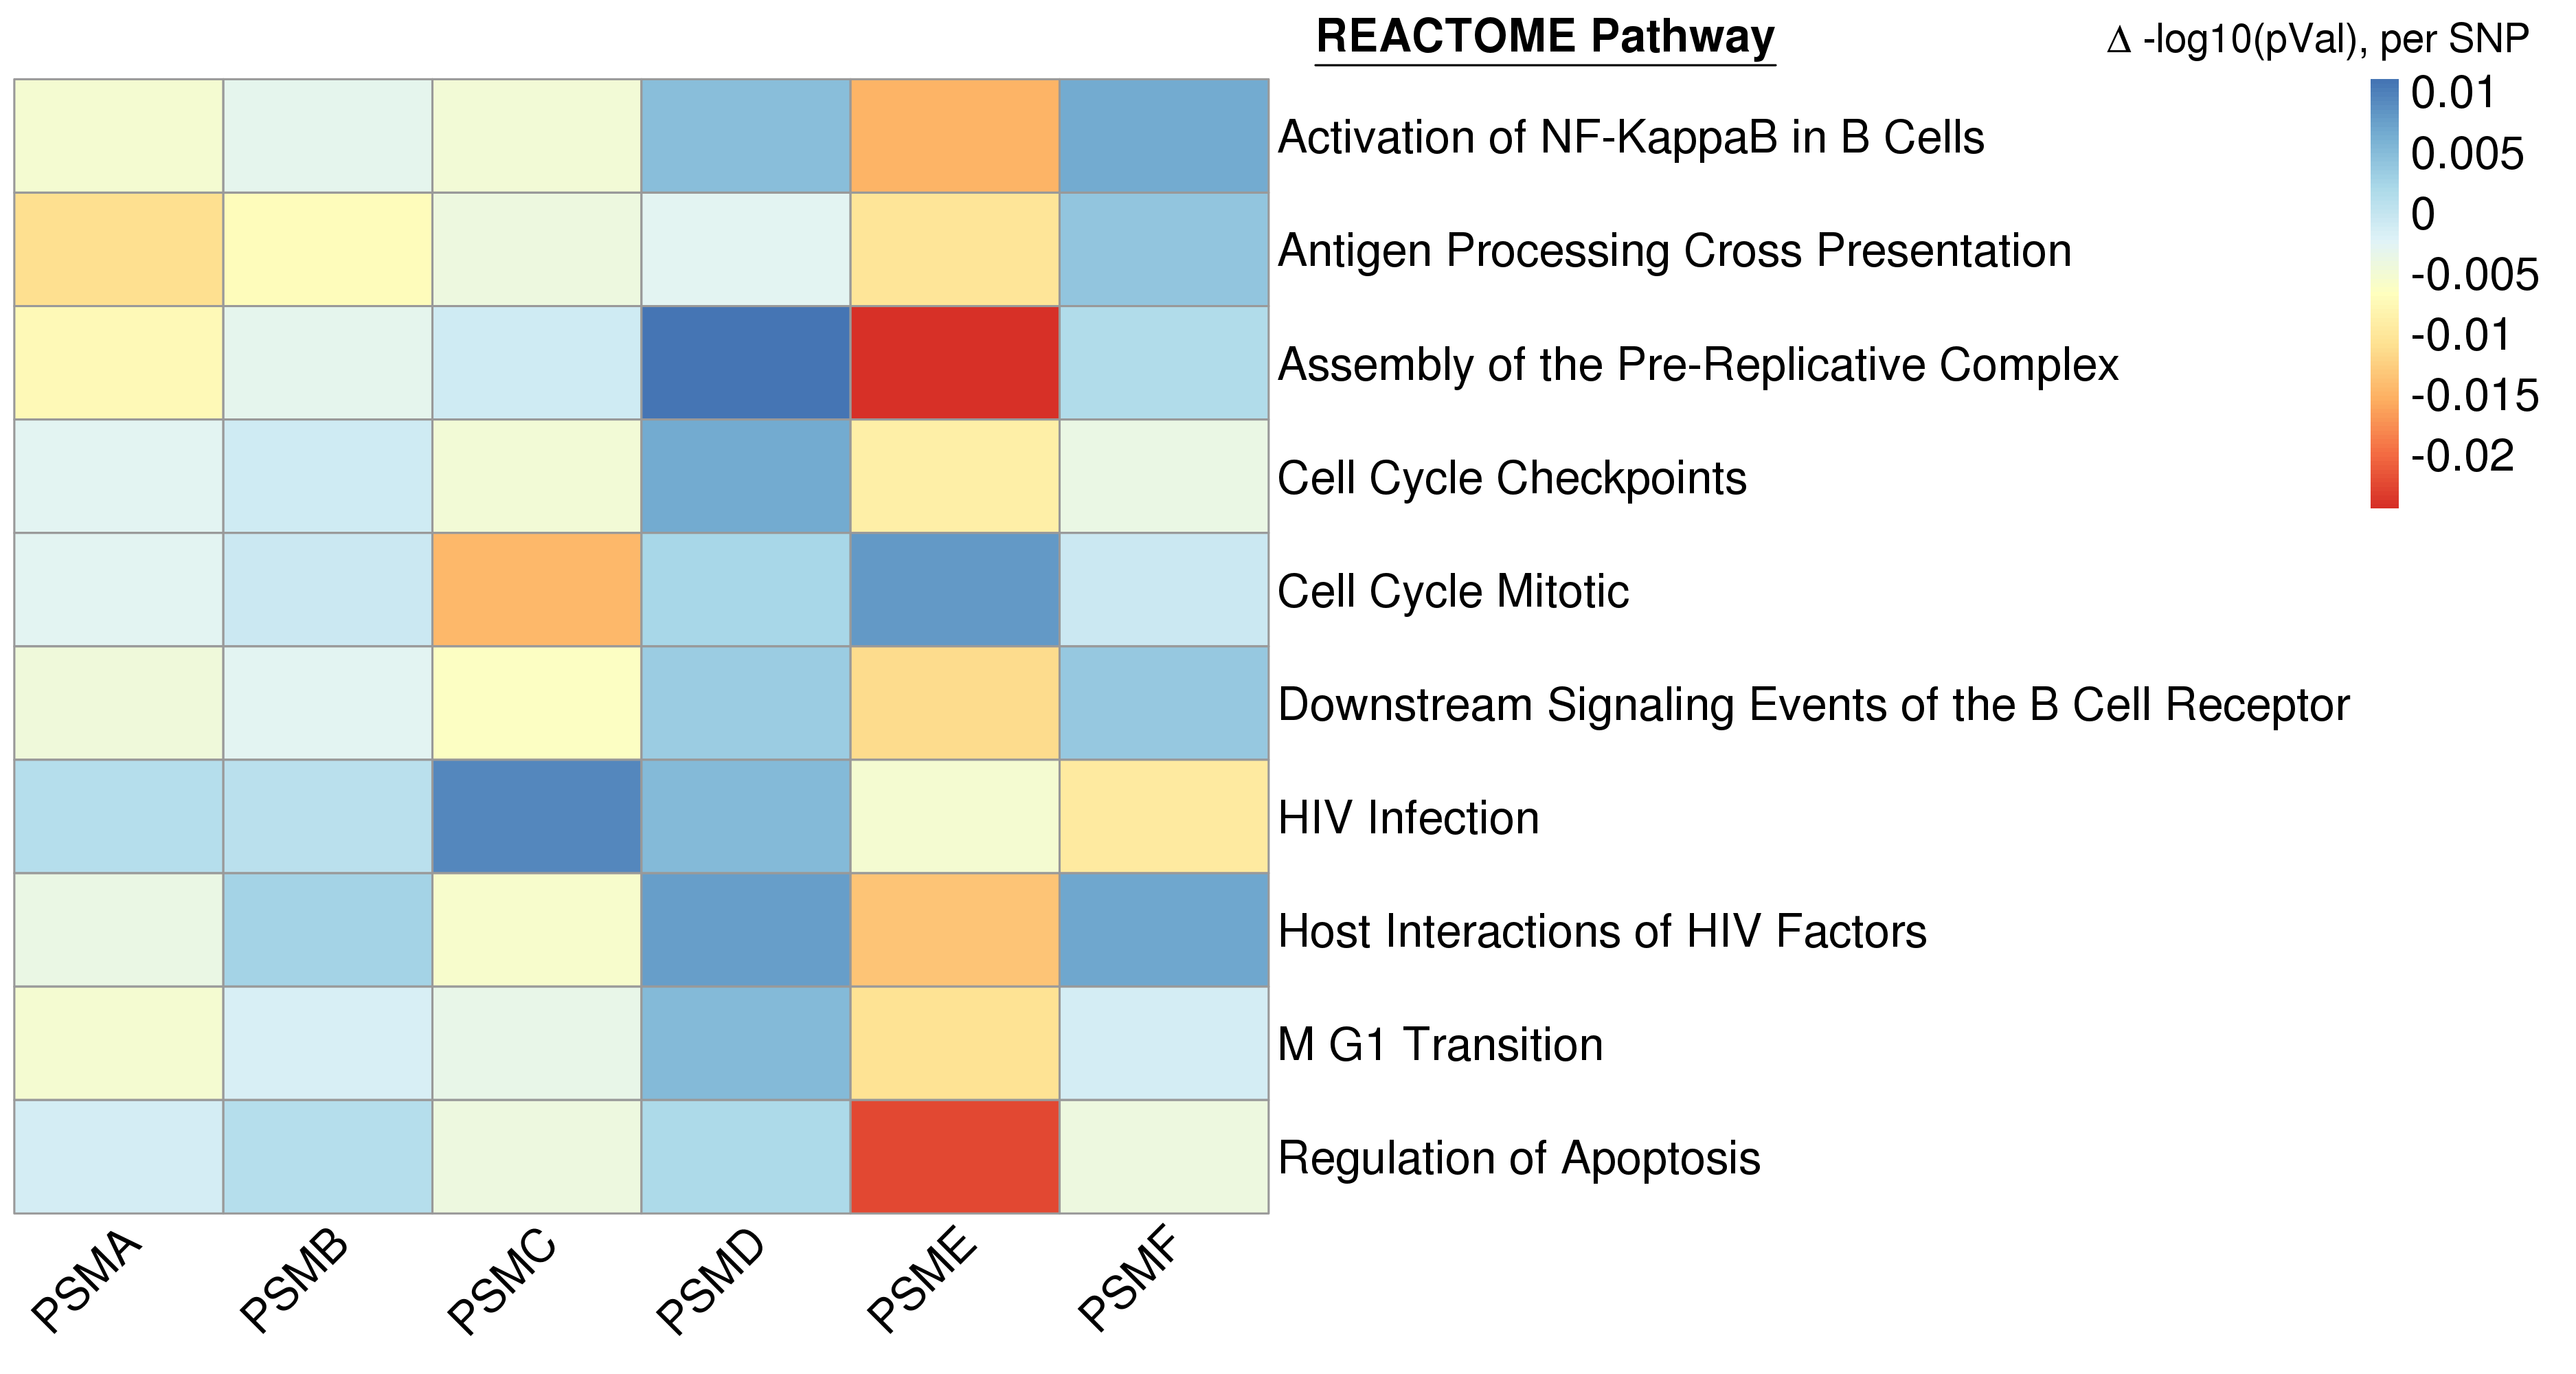
\includegraphics[scale=.5]{Images/Supp/InterPath_Supp_Figure_Proteaseome_Heatplots_BritRan4000_Loop_vs3.png}}
\par
\subfloat[]{\resizebox{1.1\columnwidth}{!}{
 \hspace*{-1.75cm}
 \begin{tabular}{cc|ccc}
  \hline
\textbf{Proteasome} & \textbf{SNPs} & \textbf{REACTOME} & \textbf{SNPs} & \textbf{MAPIT-R} \\
 \textbf{Gene Family} & & \textbf{Pathway} & & \textbf{$p$-Value} \\
  \hline
PSMA & 40 & Activation of NF-KappaB in B Cells & 756 & 2.28E-01  \\
PSMB & 91 & Antigen Processing Cross Presentation & 1104 & 2.48E-05 \\
PSMC & 29 & Assembly of the Pre-Replicative Complex & 507 & 1.84E-02 \\
PSMD & 101 & Cell Cycle Checkpoints & 1121 & 6.77E-02 \\
PSME & 25 & Cell Cycle Mitotic & 3304 & 2.34E-01 \\
 PSMF & 26 & Downstream Signaling Events of the B Cell Receptor & 1248 & 3.25E-01 \\
 & & HIV Infection & 2221 & 8.26E-02 \\
 & & Host Interactions of HIV Factors & 1541 & 1.55E-02 \\
 & & M G1 Transition & 697 & 3.02E-01 \\
 & & Regulation of Apoptosis & 906 & 2.98E-02 \\
  \hline
\end{tabular}}}
\caption[TBD]{\textbf{Proteasome gene family leave-one-out MAPIT-R reruns, REACTOME-BMI-British.Ran4000}. (a) The figure shows the change in original MAPIT-R -$\log_{10}$ $p$-value for each presented REACTOME pathway when each proteasome gene family is removed one at a time. The analyses were conducted in the BMI-British.Ran4000 subgroup combination. The $x$-axis shows each proteasome gene family and the $y$-axis shows each REACTOME pathway. Each column has been scaled by the number of SNPs present in the given gene family and, as a result, the heatplot specifically shows the -$\log_{10}$ $p$-value change per SNP. (b) The table shows the number of SNPs that are present in each proteasome gene family (left) and each REACTOME pathway (right). The original MAPIT-R $p$-values for each pathway are also shown (right).}
\label{InterPath-Supp-Figure-Prot-Heatplots-BritRan4000}
\end{figure}
\clearpage
\addtocounter{figure}{-1}
\addtocounter{CharNumber5}{1}

\begin{figure}[ht]
\centering
\vspace*{-.5cm}
\subfloat[]{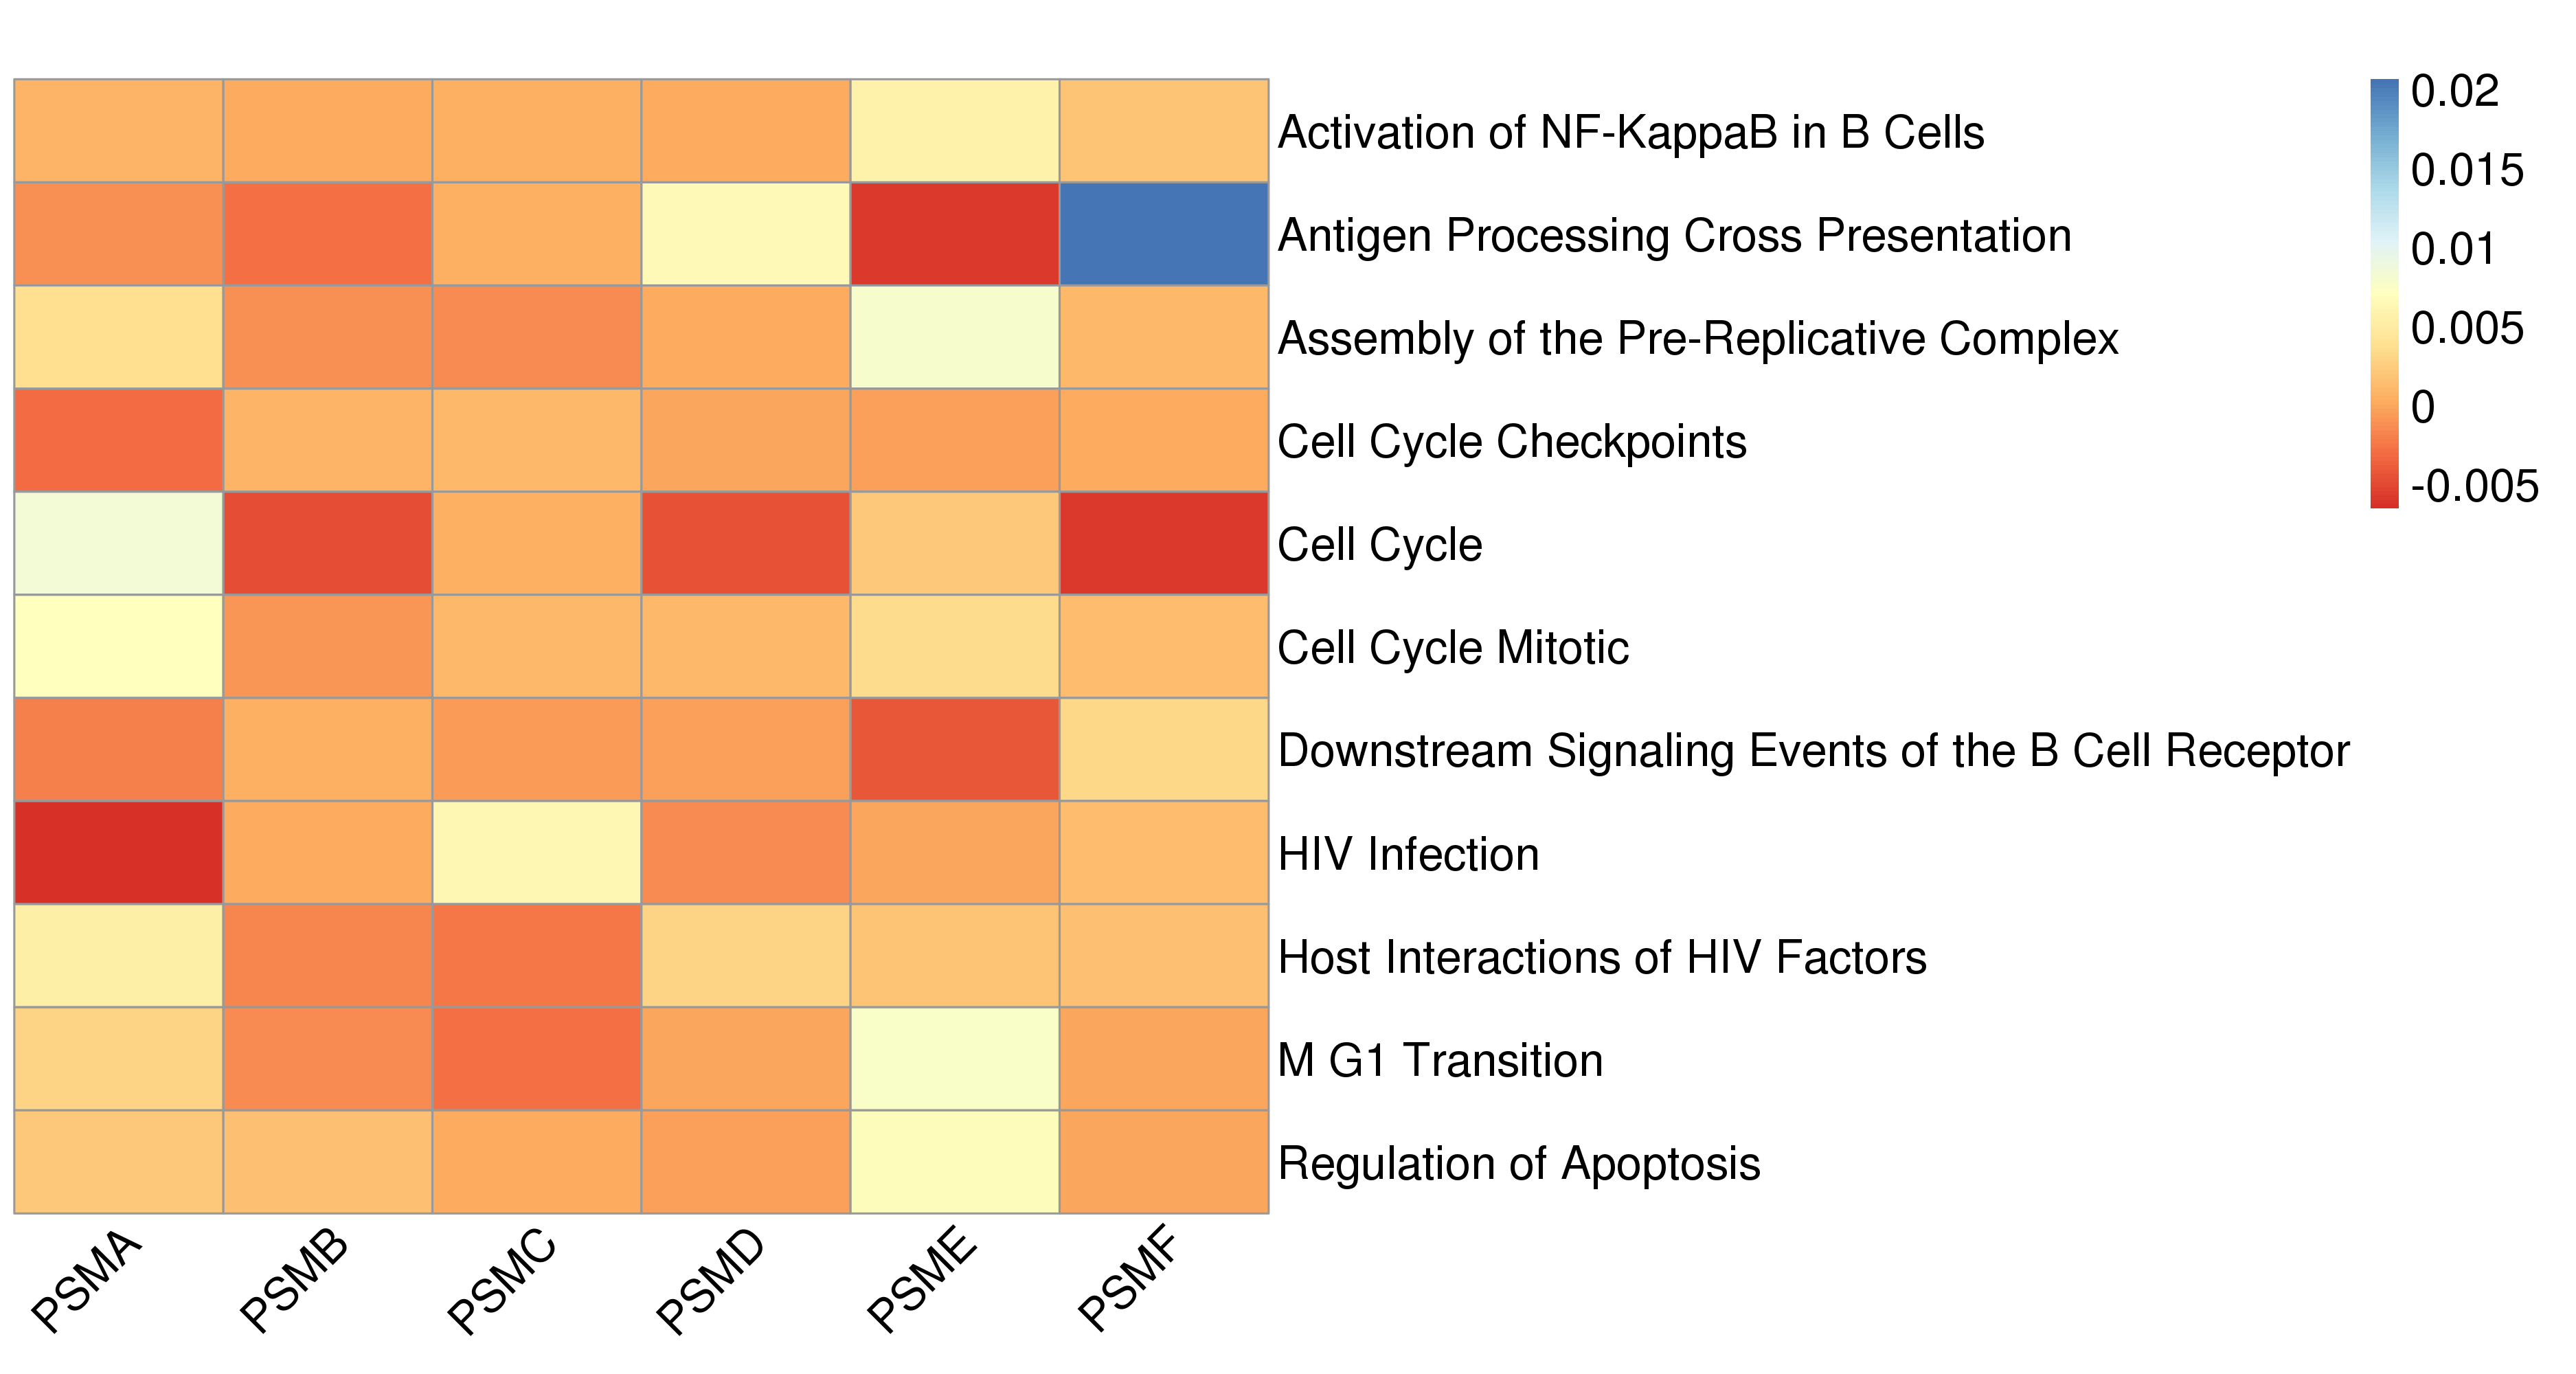
\includegraphics[scale=.5]{Images/Supp/InterPath_Supp_Figure_Proteaseome_Heatplots_Caribbean_Loop_vs3.png}}
\par
\subfloat[]{\resizebox{1.1\columnwidth}{!}{
 \hspace*{-1.75cm}
 \begin{tabular}{cc|ccc}
  \hline
\textbf{Proteasome} & \textbf{SNPs} & \textbf{REACTOME} & \textbf{SNPs} & \textbf{MAPIT-R} \\
 \textbf{Gene Family} & & \textbf{Pathway} & & \textbf{$p$-Value} \\
  \hline
PSMA & 18 & Activation of NF-KappaB in B Cells & 507 & 9.93E-01  \\
PSMB & 77 & Antigen Processing Cross Presentation & 871 & 5.15E-02 \\
PSMC & 21 & Assembly of the Pre-Replicative Complex & 357 & 7.25E-01 \\
PSMD & 69 & Cell Cycle Checkpoints & 736 & 8.83E-01 \\
PSME & 15 & Cell Cycle & 2711 & 2.51E-01 \\
PSMF & 16 & Cell Cycle Mitotic & 2111 & 7.98E-01 \\
 & & Downstream Signaling Events of the B Cell Receptor & 829 & 8.37E-01 \\
 & & HIV Infection & 1483 & 3.11E-01 \\
 & & Host Interactions of HIV Factors & 1055 & 6.68E-01 \\
 & & M G1 Transition & 500 & 6.37E-01 \\
 & & Regulation of Apoptosis & 615 & 9.42E-01 \\
  \hline
\end{tabular}}}
\caption[TBD]{\textbf{Proteasome gene family leave-one-out MAPIT-R reruns, REACTOME-BMI-Caribbean}. (a) The figure shows the change in original MAPIT-R -$\log_{10}$ $p$-value for each presented REACTOME pathway when each proteasome gene family is removed one at a time. The analyses were conducted in the BMI-Caribbean subgroup combination. The $x$-axis shows each proteasome gene family and the $y$-axis shows each REACTOME pathway. Each column has been scaled by the number of SNPs present in the given gene family and, as a result, the heatplot specifically shows the -$\log_{10}$ $p$-value change per SNP. (b) The table shows the number of SNPs that are present in each proteasome gene family (left) and each REACTOME pathway (right). The original MAPIT-R $p$-values for each pathway are also shown (right).}
\label{InterPath-Supp-Figure-Prot-Heatplots-Caribbean}
\end{figure}
\clearpage
\addtocounter{figure}{-1}
\addtocounter{CharNumber5}{1}

\begin{figure}[ht]
\centering
\vspace*{-.5cm}
\subfloat[]{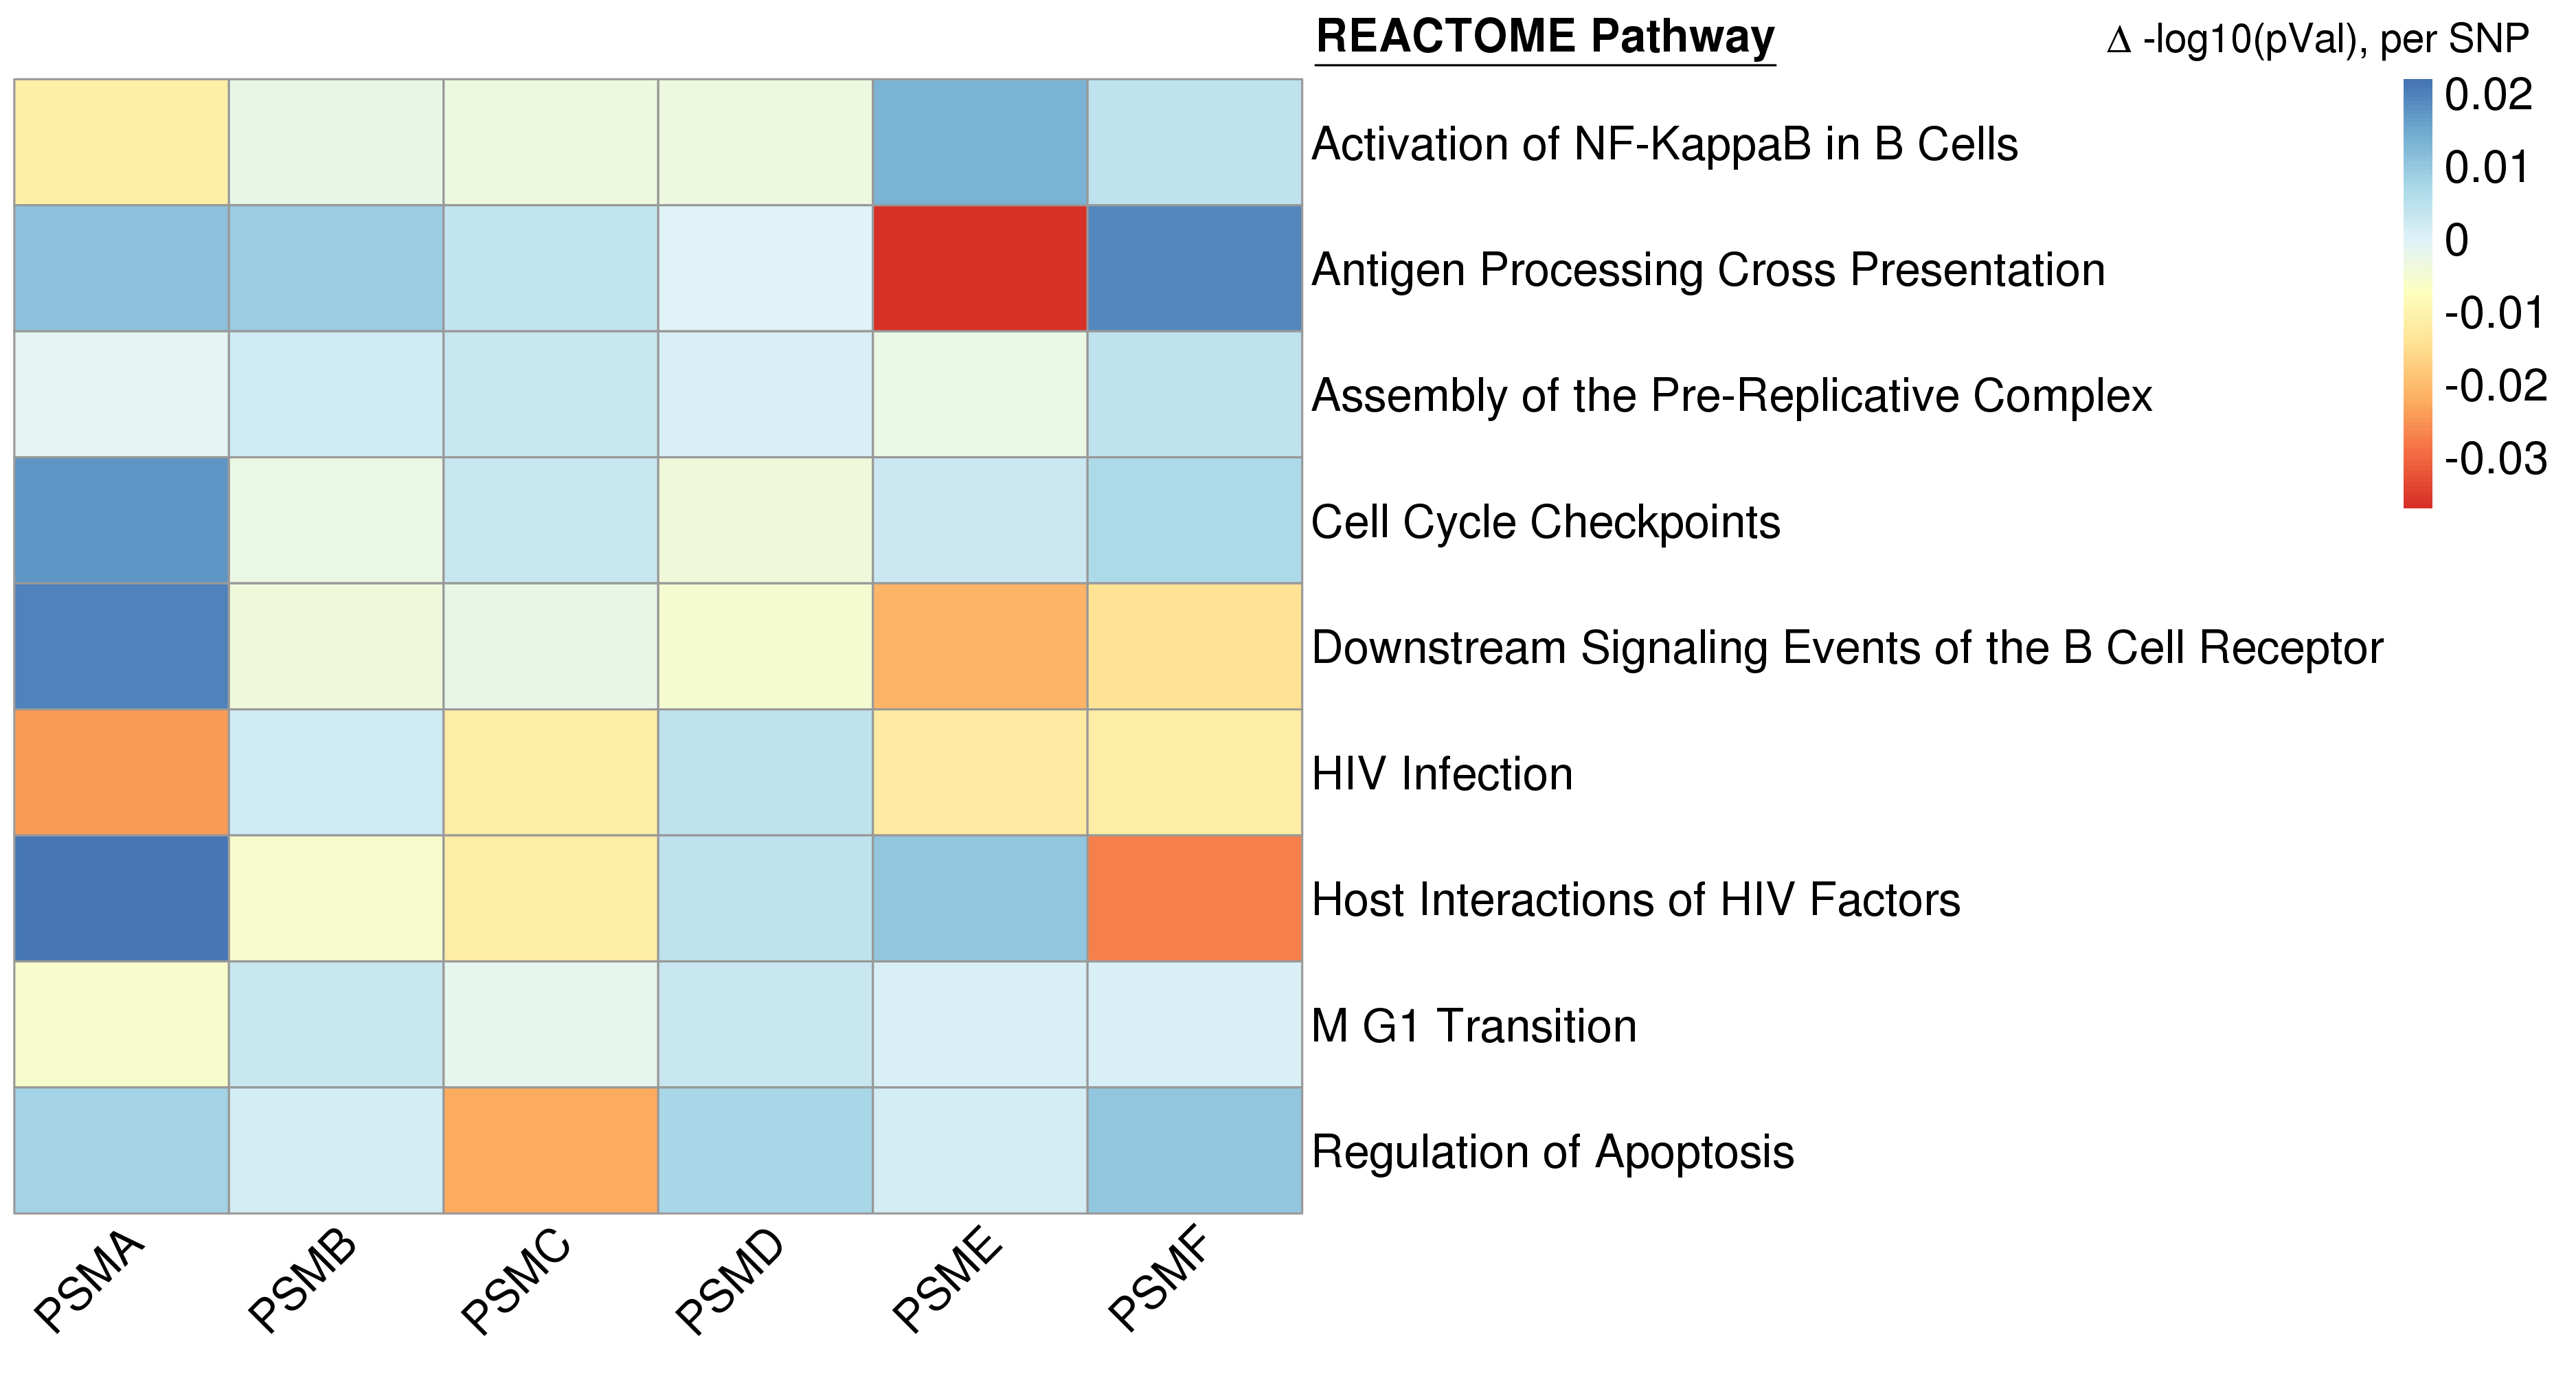
\includegraphics[scale=.5]{Images/Supp/InterPath_Supp_Figure_Proteaseome_Heatplots_Chinese_Loop_vs3.png}}
\par
\subfloat[]{\resizebox{1.1\columnwidth}{!}{
 \hspace*{-1.75cm}
 \begin{tabular}{cc|ccc}
  \hline
\textbf{Proteasome} & \textbf{SNPs} & \textbf{REACTOME} & \textbf{SNPs} & \textbf{MAPIT-R} \\
 \textbf{Gene Family} & & \textbf{Pathway} & & \textbf{$p$-Value} \\
  \hline
PSMA & 13 & Activation of NF-KappaB in B Cells & 433 & 5.27E-01  \\
PSMB & 74 & Antigen Processing Cross Presentation & 771 & 1.11E-02 \\
PSMC & 18 & Assembly of the Pre-Replicative Complex & 292 & 8.77E-01 \\
PSMD & 58 & Cell Cycle Checkpoints & 589 & 5.41E-01  \\
PSME & 12 & Downstream Signaling Events of the B Cell Receptor & 698 & 1.40E-01 \\
PSMF & 16 & HIV Infection & 1266 & 3.68E-03 \\
 & & Host Interactions of HIV Factors & 902 & 4.24E-02 \\
 & & M G1 Transition & 400 & 8.20E-01 \\
 & & Regulation of Apoptosis & 527 & 2.26E-02 \\
  \hline
\end{tabular}}}
\caption[TBD]{\textbf{Proteasome gene family leave-one-out MAPIT-R reruns, REACTOME-BMI-Chinese}. (a) The figure shows the change in original MAPIT-R -$\log_{10}$ $p$-value for each presented REACTOME pathway when each proteasome gene family is removed one at a time. The analyses were conducted in the BMI-Chinese subgroup combination. The $x$-axis shows each proteasome gene family and the $y$-axis shows each REACTOME pathway. Each column has been scaled by the number of SNPs present in the given gene family and, as a result, the heatplot specifically shows the -$\log_{10}$ $p$-value change per SNP. (b) The table shows the number of SNPs that are present in each proteasome gene family (left) and each REACTOME pathway (right). The original MAPIT-R $p$-values for each pathway are also shown (right).}
\label{InterPath-Supp-Figure-Prot-Heatplots-Chinese}
\end{figure}
\clearpage
\addtocounter{figure}{-1}
\addtocounter{CharNumber5}{1}

\begin{figure}[ht]
\centering
\vspace*{-.5cm}
\subfloat[]{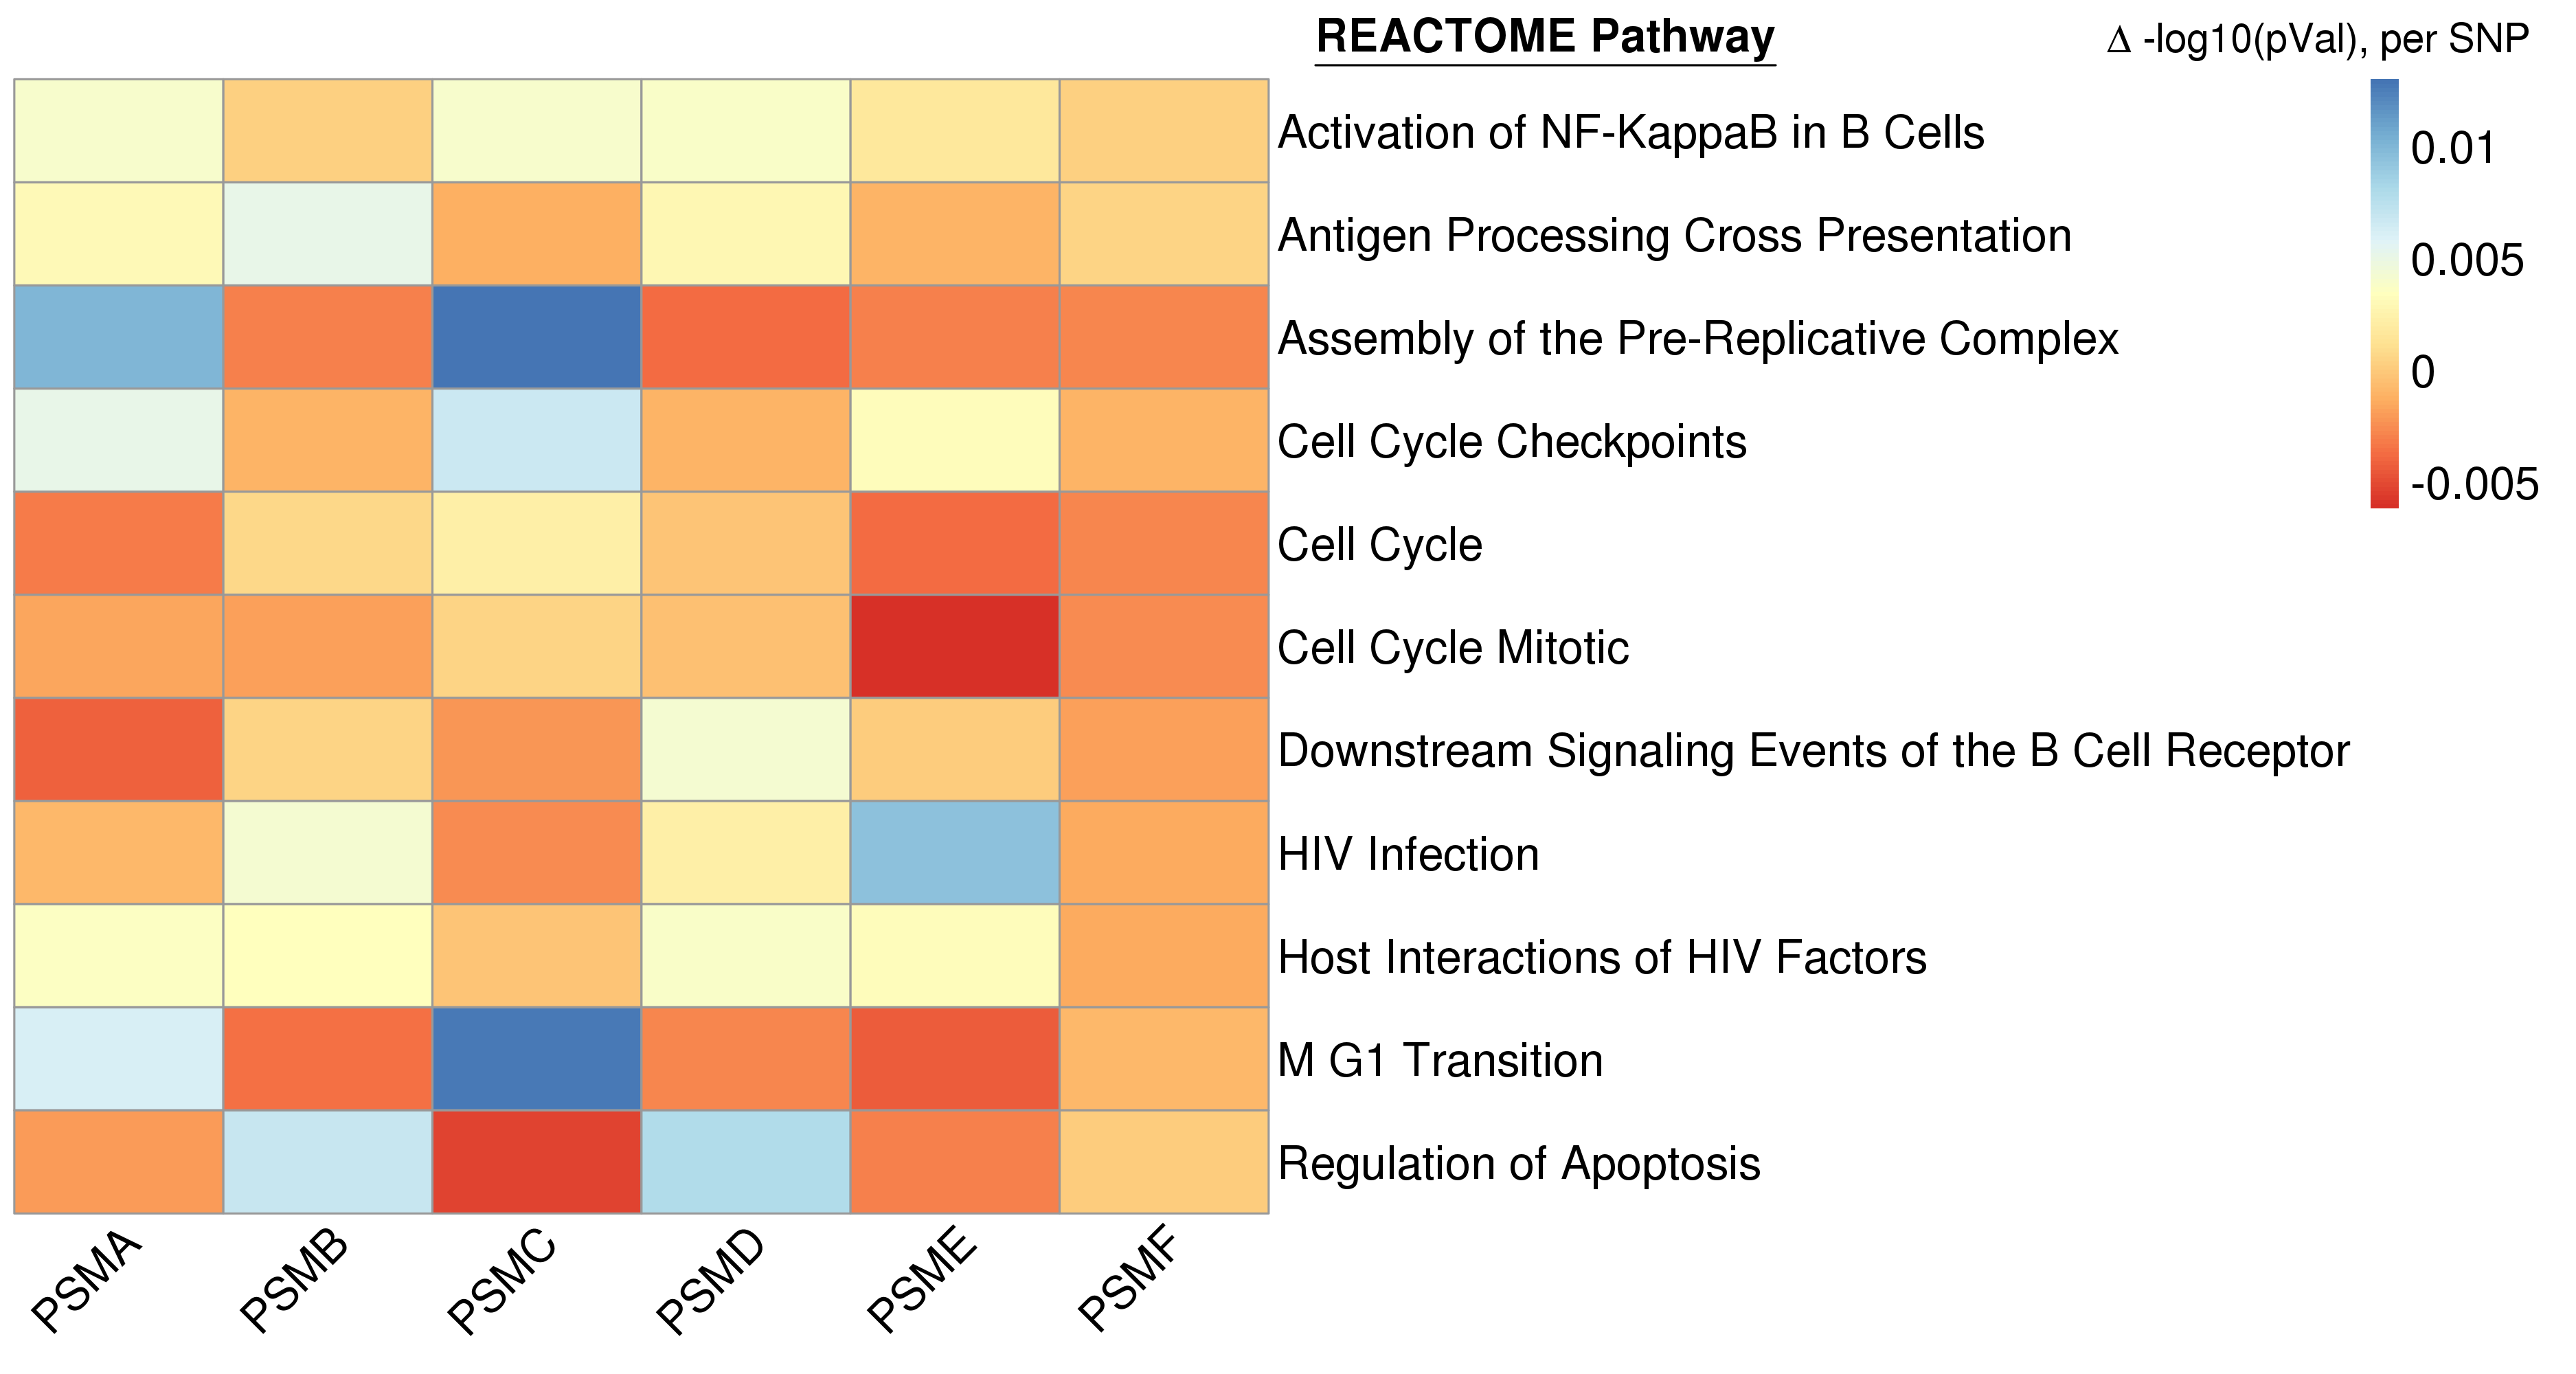
\includegraphics[scale=.5]{Images/Supp/InterPath_Supp_Figure_Proteaseome_Heatplots_Indian_Loop_vs3.png}}
\par
\subfloat[]{\resizebox{1.1\columnwidth}{!}{
 \hspace*{-1.75cm}
 \begin{tabular}{cc|ccc}
  \hline
\textbf{Proteasome} & \textbf{SNPs} & \textbf{REACTOME} & \textbf{SNPs} & \textbf{MAPIT-R} \\
 \textbf{Gene Family} & & \textbf{Pathway} & & \textbf{$p$-Value} \\
  \hline
PSMA & 29 & Activation of NF-KappaB in B Cells & 618 & 9.978E-01  \\
PSMB & 85 & Antigen Processing Cross Presentation & 977 & 4.476E-01 \\
PSMC & 25 & Assembly of the Pre-Replicative Complex & 427 & 5.019E-01 \\
PSMD & 78 & Cell Cycle Checkpoints & 909 & 8.042E-01 \\
PSME & 21 & Cell Cycle & 3361 & 1.873E-01 \\
PSMF & 21 & Cell Cycle Mitotic & 2656 & 2.316E-01 \\
 & & Downstream Signaling Events of the B Cell Receptor & 1037 & 5.534E-01 \\
 & & HIV Infection & 1836 & 9.803E-02 \\
 & & Host Interactions of HIV Factors & 1278 & 3.788E-01 \\
 & & M G1 Transition & 590 & 4.658E-01 \\
 & & Regulation of Apoptosis & 754 & 5.606E-01 \\
  \hline
\end{tabular}}}
\caption[TBD]{\textbf{Proteasome gene family leave-one-out MAPIT-R reruns, REACTOME-BMI-Indian}. (a) The figure shows the change in original MAPIT-R -$\log_{10}$ $p$-value for each presented REACTOME pathway when each proteasome gene family is removed one at a time. The analyses were conducted in the BMI-Indian subgroup combination. The $x$-axis shows each proteasome gene family and the $y$-axis shows each REACTOME pathway. Each column has been scaled by the number of SNPs present in the given gene family and, as a result, the heatplot specifically shows the -$\log_{10}$ $p$-value change per SNP. (b) The table shows the number of SNPs that are present in each proteasome gene family (left) and each REACTOME pathway (right). The original MAPIT-R $p$-values for each pathway are also shown (right).}
\label{InterPath-Supp-Figure-Prot-Heatplots-Indian}
\end{figure}
\clearpage
\addtocounter{figure}{-1}
\addtocounter{CharNumber5}{1}

\begin{figure}[ht]
\centering
\vspace*{-.5cm}
\subfloat[]{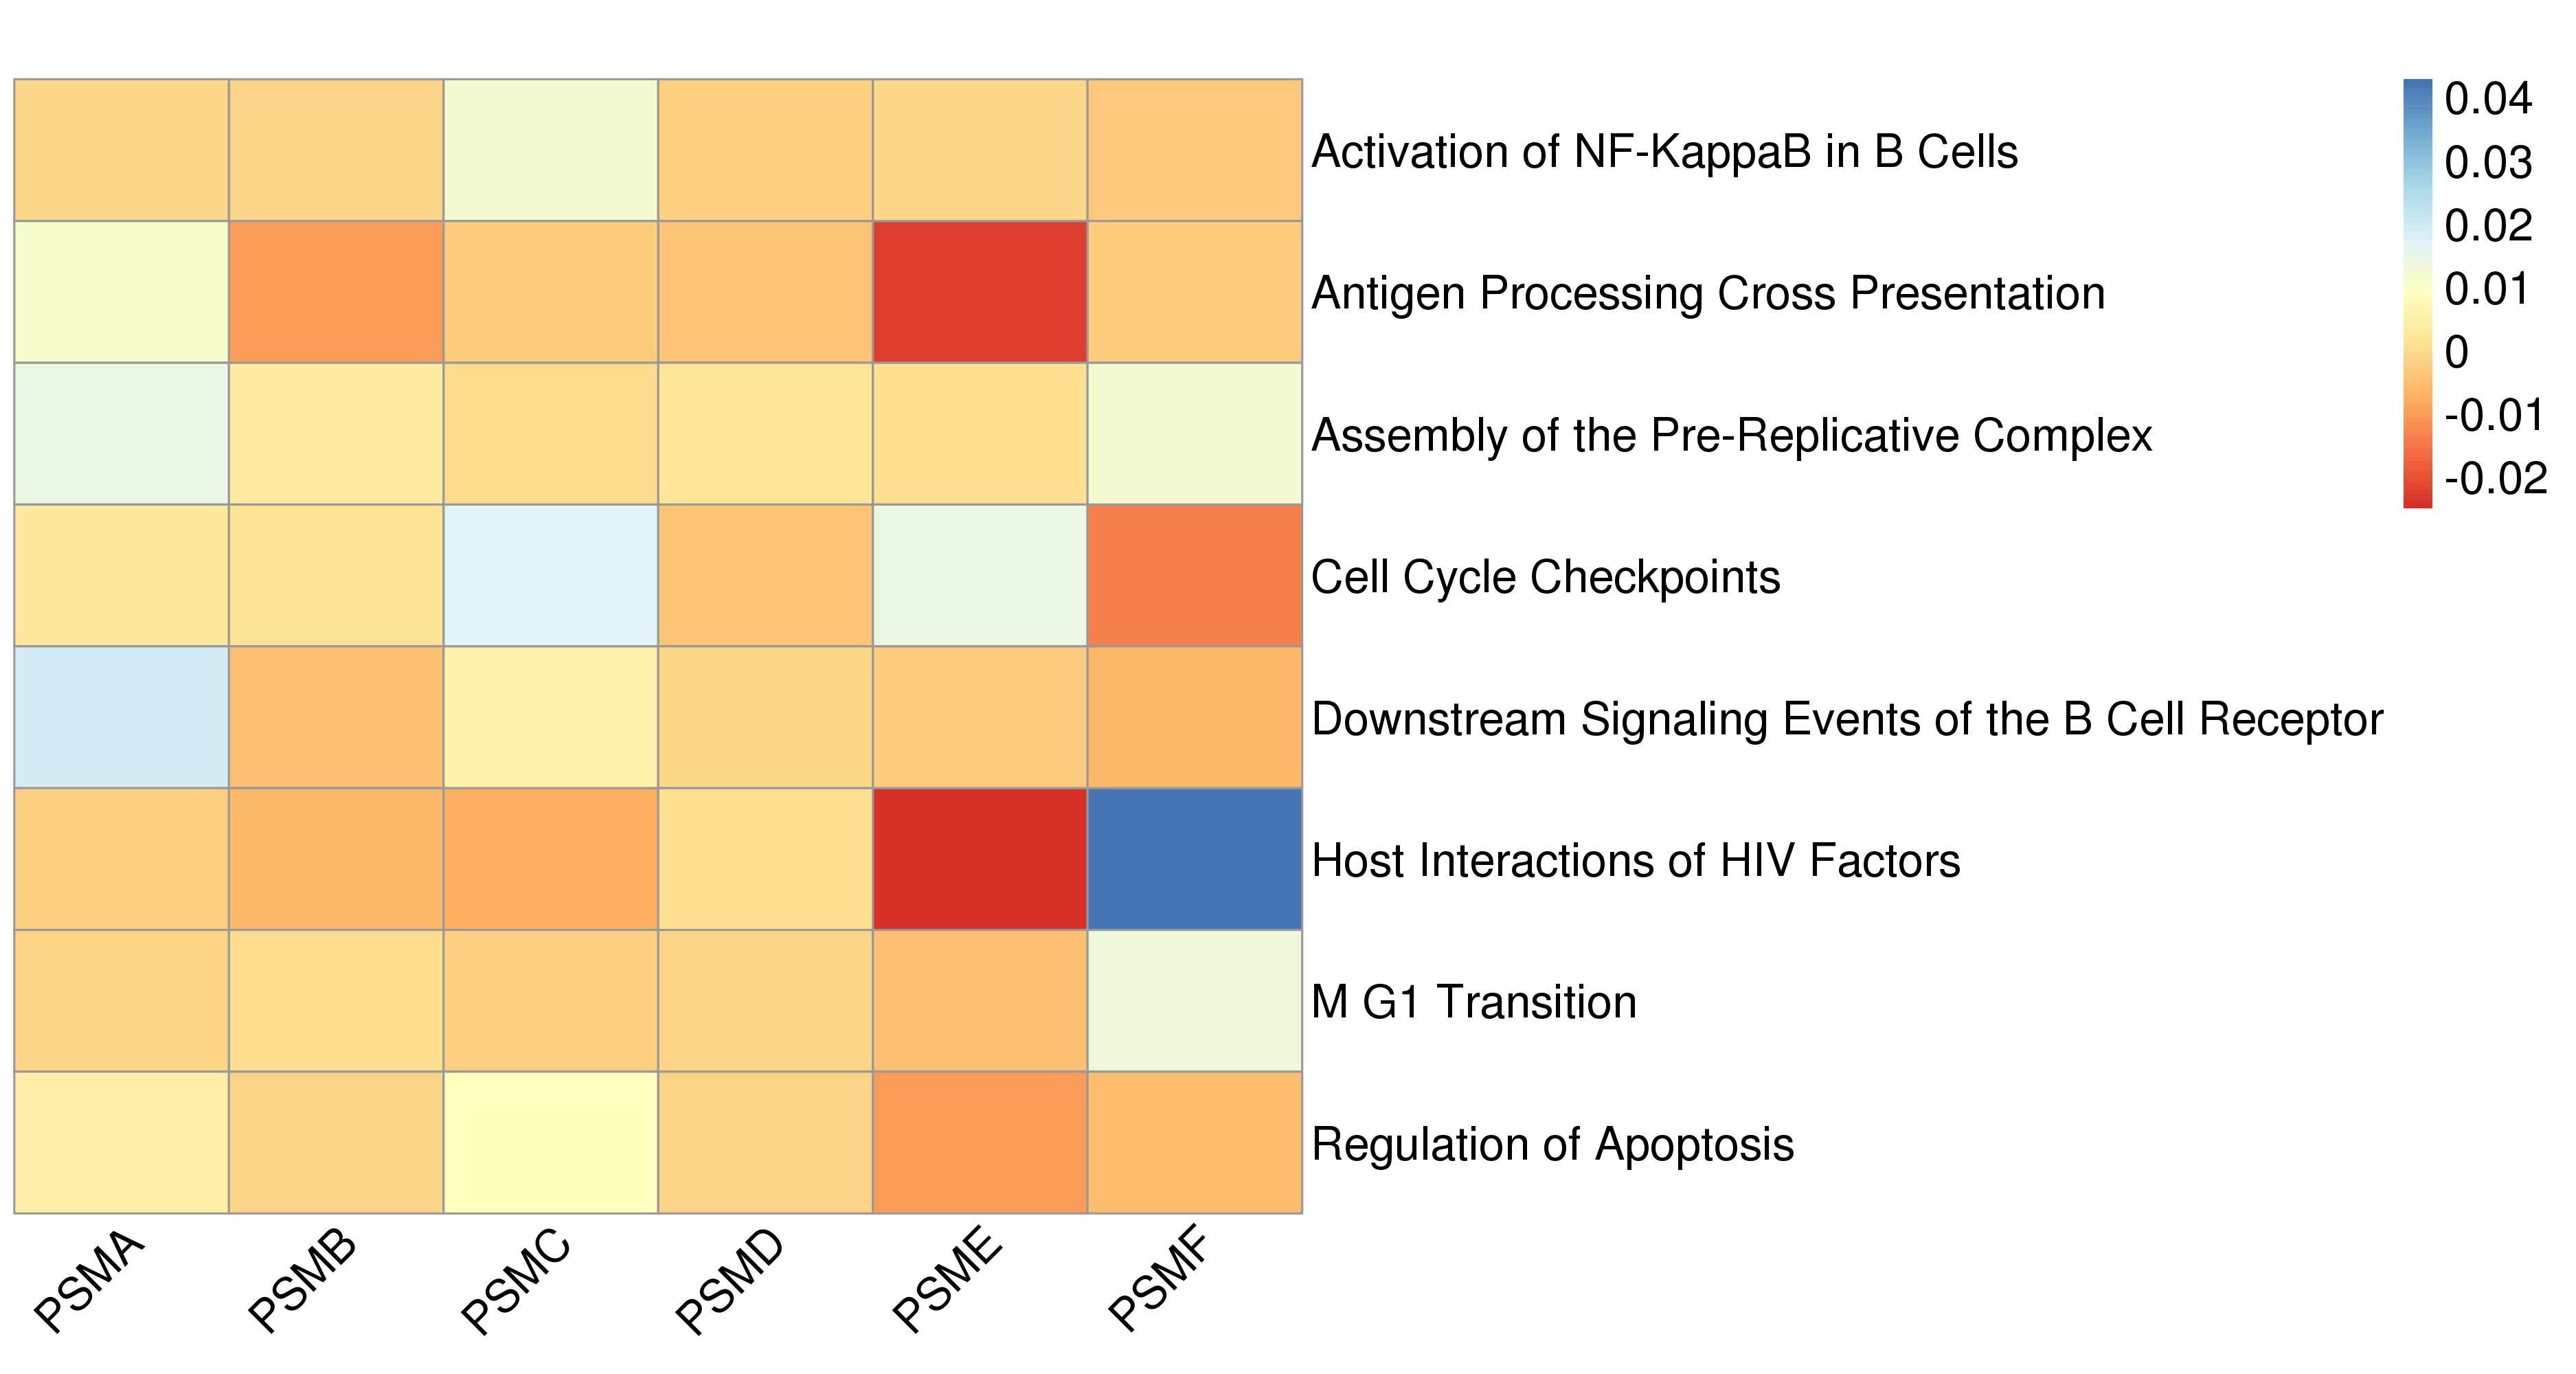
\includegraphics[scale=.5]{Images/Supp/InterPath_Supp_Figure_Proteaseome_Heatplots_Pakistani_Loop_vs3.png}}
\par
\subfloat[]{\resizebox{1.1\columnwidth}{!}{
 \hspace*{-1.75cm}
 \begin{tabular}{cc|ccc}
  \hline
\textbf{Proteasome} & \textbf{SNPs} & \textbf{REACTOME} & \textbf{SNPs} & \textbf{MAPIT-R} \\
 \textbf{Gene Family} & & \textbf{Pathway} & & \textbf{$p$-Value} \\
  \hline
PSMA & 30 & Activation of NF-KappaB in B Cells & 643 & 4.61E-01  \\
PSMB & 90 & Antigen Processing Cross Presentation & 1036 & 8.74E-03 \\
PSMC & 24 & Assembly of the Pre-Replicative Complex & 444 & 9.73E-01 \\
PSMD & 86 & Cell Cycle Checkpoints & 940 & 1.63E-01 \\
PSME & 21 & Downstream Signaling Events of the B Cell Receptor & 1073 & 6.57E-02 \\
PSMF & 22 & Host Interactions of HIV Factors & 1315 & 1.00E-01 \\
 & & M G1 Transition & 612 & 6.66E-01 \\
 & & Regulation of Apoptosis & 774 & 5.16E-02 \\
  \hline
\end{tabular}}}
\caption[TBD]{\textbf{Proteasome gene family leave-one-out MAPIT-R reruns, REACTOME-BMI-Pakistani}. (a) The figure shows the change in original MAPIT-R -$\log_{10}$ $p$-value for each presented REACTOME pathway when each proteasome gene family is removed one at a time. The analyses were conducted in the BMI-Pakistani subgroup combination. The $x$-axis shows each proteasome gene family and the $y$-axis shows each REACTOME pathway. Each column has been scaled by the number of SNPs present in the given gene family and, as a result, the heatplot specifically shows the -$\log_{10}$ $p$-value change per SNP. (b) The table shows the number of SNPs that are present in each proteasome gene family (left) and each REACTOME pathway (right). The original MAPIT-R $p$-values for each pathway are also shown (right).}
\label{InterPath-Supp-Figure-Prot-Heatplots-Pakistani}
\end{figure}
\clearpage
\addtocounter{figure}{-1}
\addtocounter{CharNumber5}{1}

\addtocounter{figure}{1}
\renewcommand{\thefigure}{\arabic{figure}}

\setlength{\footskip}{3cm}
\begin{figure}[htbp]
\centering
\vspace*{-2cm}
\includegraphics[scale=.2]{Images/Supp/InterPath_Supp_Figure_IBS_AllPops_vs4_noHLA.png}
\caption[TBD]{\textbf{Pathway-level genetic diversity vs. MAPIT-R results for all database-phenotype-subgroup combinations}. Caption continued on next page.}
\label{InterPath-Supp-Figure-IBS-AllPops}
\end{figure}
\clearpage
\setlength{\footskip}{1cm}
\addtocounter{figure}{-1}

\begin{figure} [t!]
\caption[TBD]{\textbf{Pathway-level genetic diversity vs. MAPIT-R results for all database-phenotype-subgroup combinations}. The figure shows the mean pairwise IBS proportions per pathway plotted against each pathway's MAPIT-R $p$-value for every pathway database-phenotype-UKB subgroup combination. IBS proportions were calculated per pathway by using that pathway's set of SNPs, were calculated pairwise between every set of individuals in the subgroup, and then averaged across each of these pairs for a final, single summary metric. We observe across the majority of combinations no significant relationship between mean pairwise IBS proportion and MAPIT-R $p$-value.}
\label{InterPath-Supp-Figure-IBS-AllPops-Caption}
\end{figure}
\clearpage

%\begin{figure}[htbp]
%\centering
%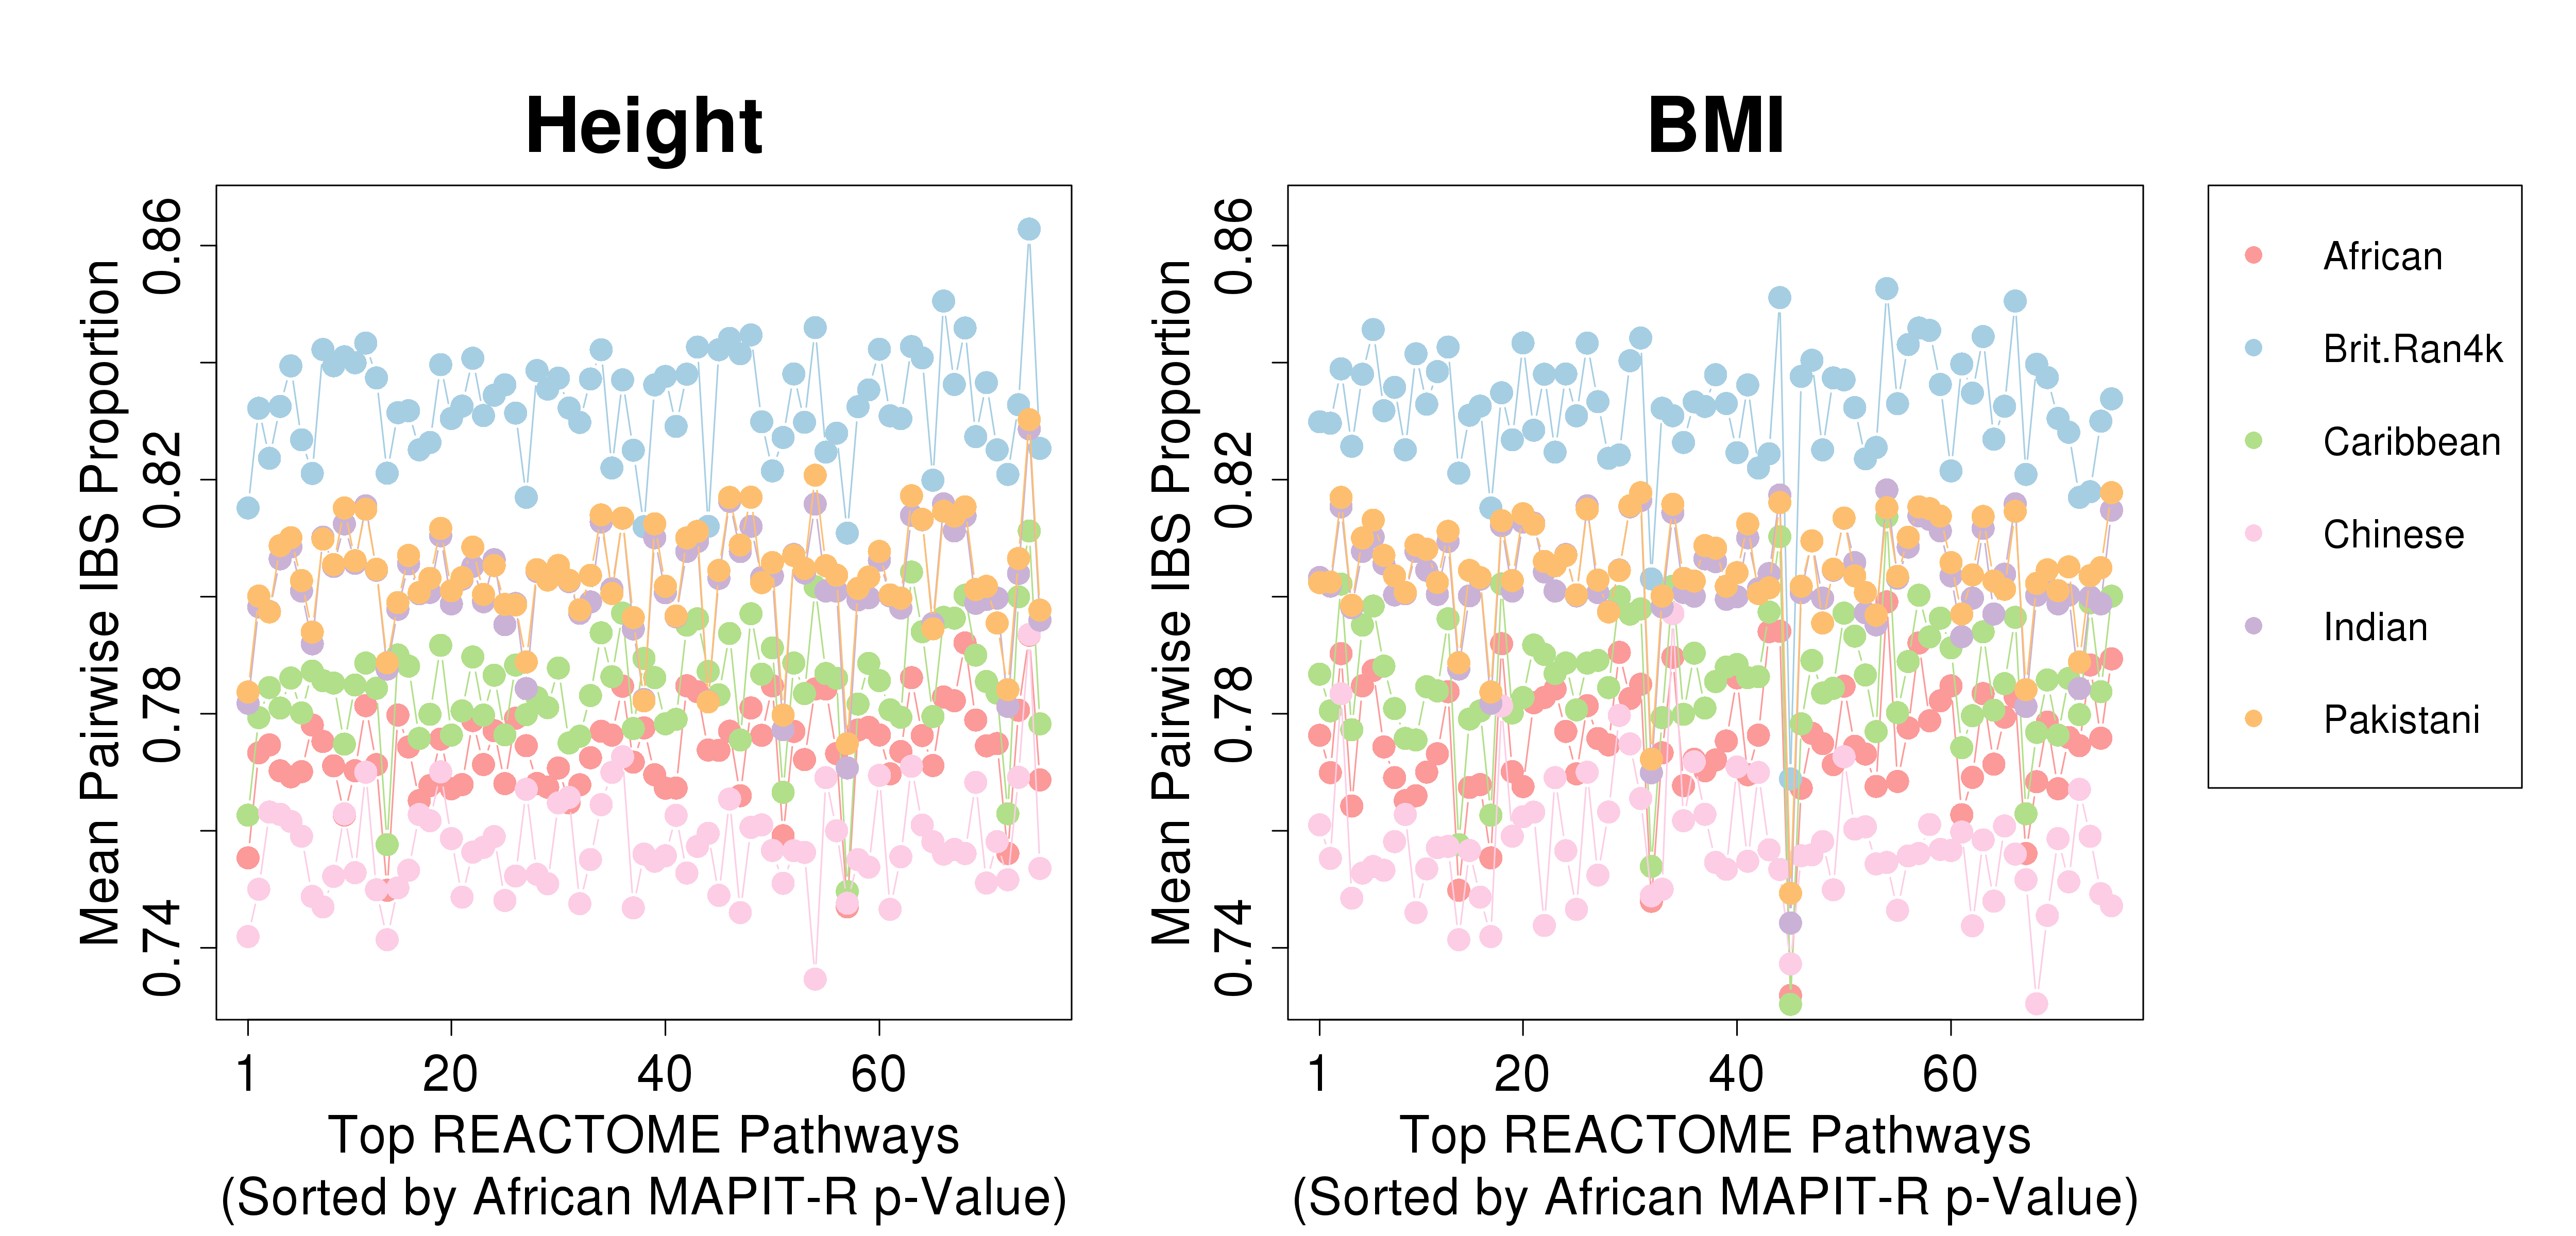
\includegraphics[scale=.35]{Images/Supp/InterPath_Supp_Figure_IBS_AllPopComps_vs3_REACTOME.png}
%\caption[TBD]{\textbf{Pathway-level genetic diversity across all UKB subgroups for top African MAPIT-R REACTOME pathways}. The figure plots the mean pairwise IBS proportions of each UKB subgroup for the top 75 REACTOME pathways (sorted by MAPIT-R African subgroup $p$-value) for each pathway database-phenotype combination. Most variation in mean pairwise IBS proportions varies moreso based on the pathways themselves and not on ancestry; subgroups differ between one another mostly at the same levels across each pathway.}
%\label{InterPath-Supp-Figure-IBS-AllPopComps-REACTOME}
%\end{figure}
%\clearpage

\begin{figure}[htbp]
\centering
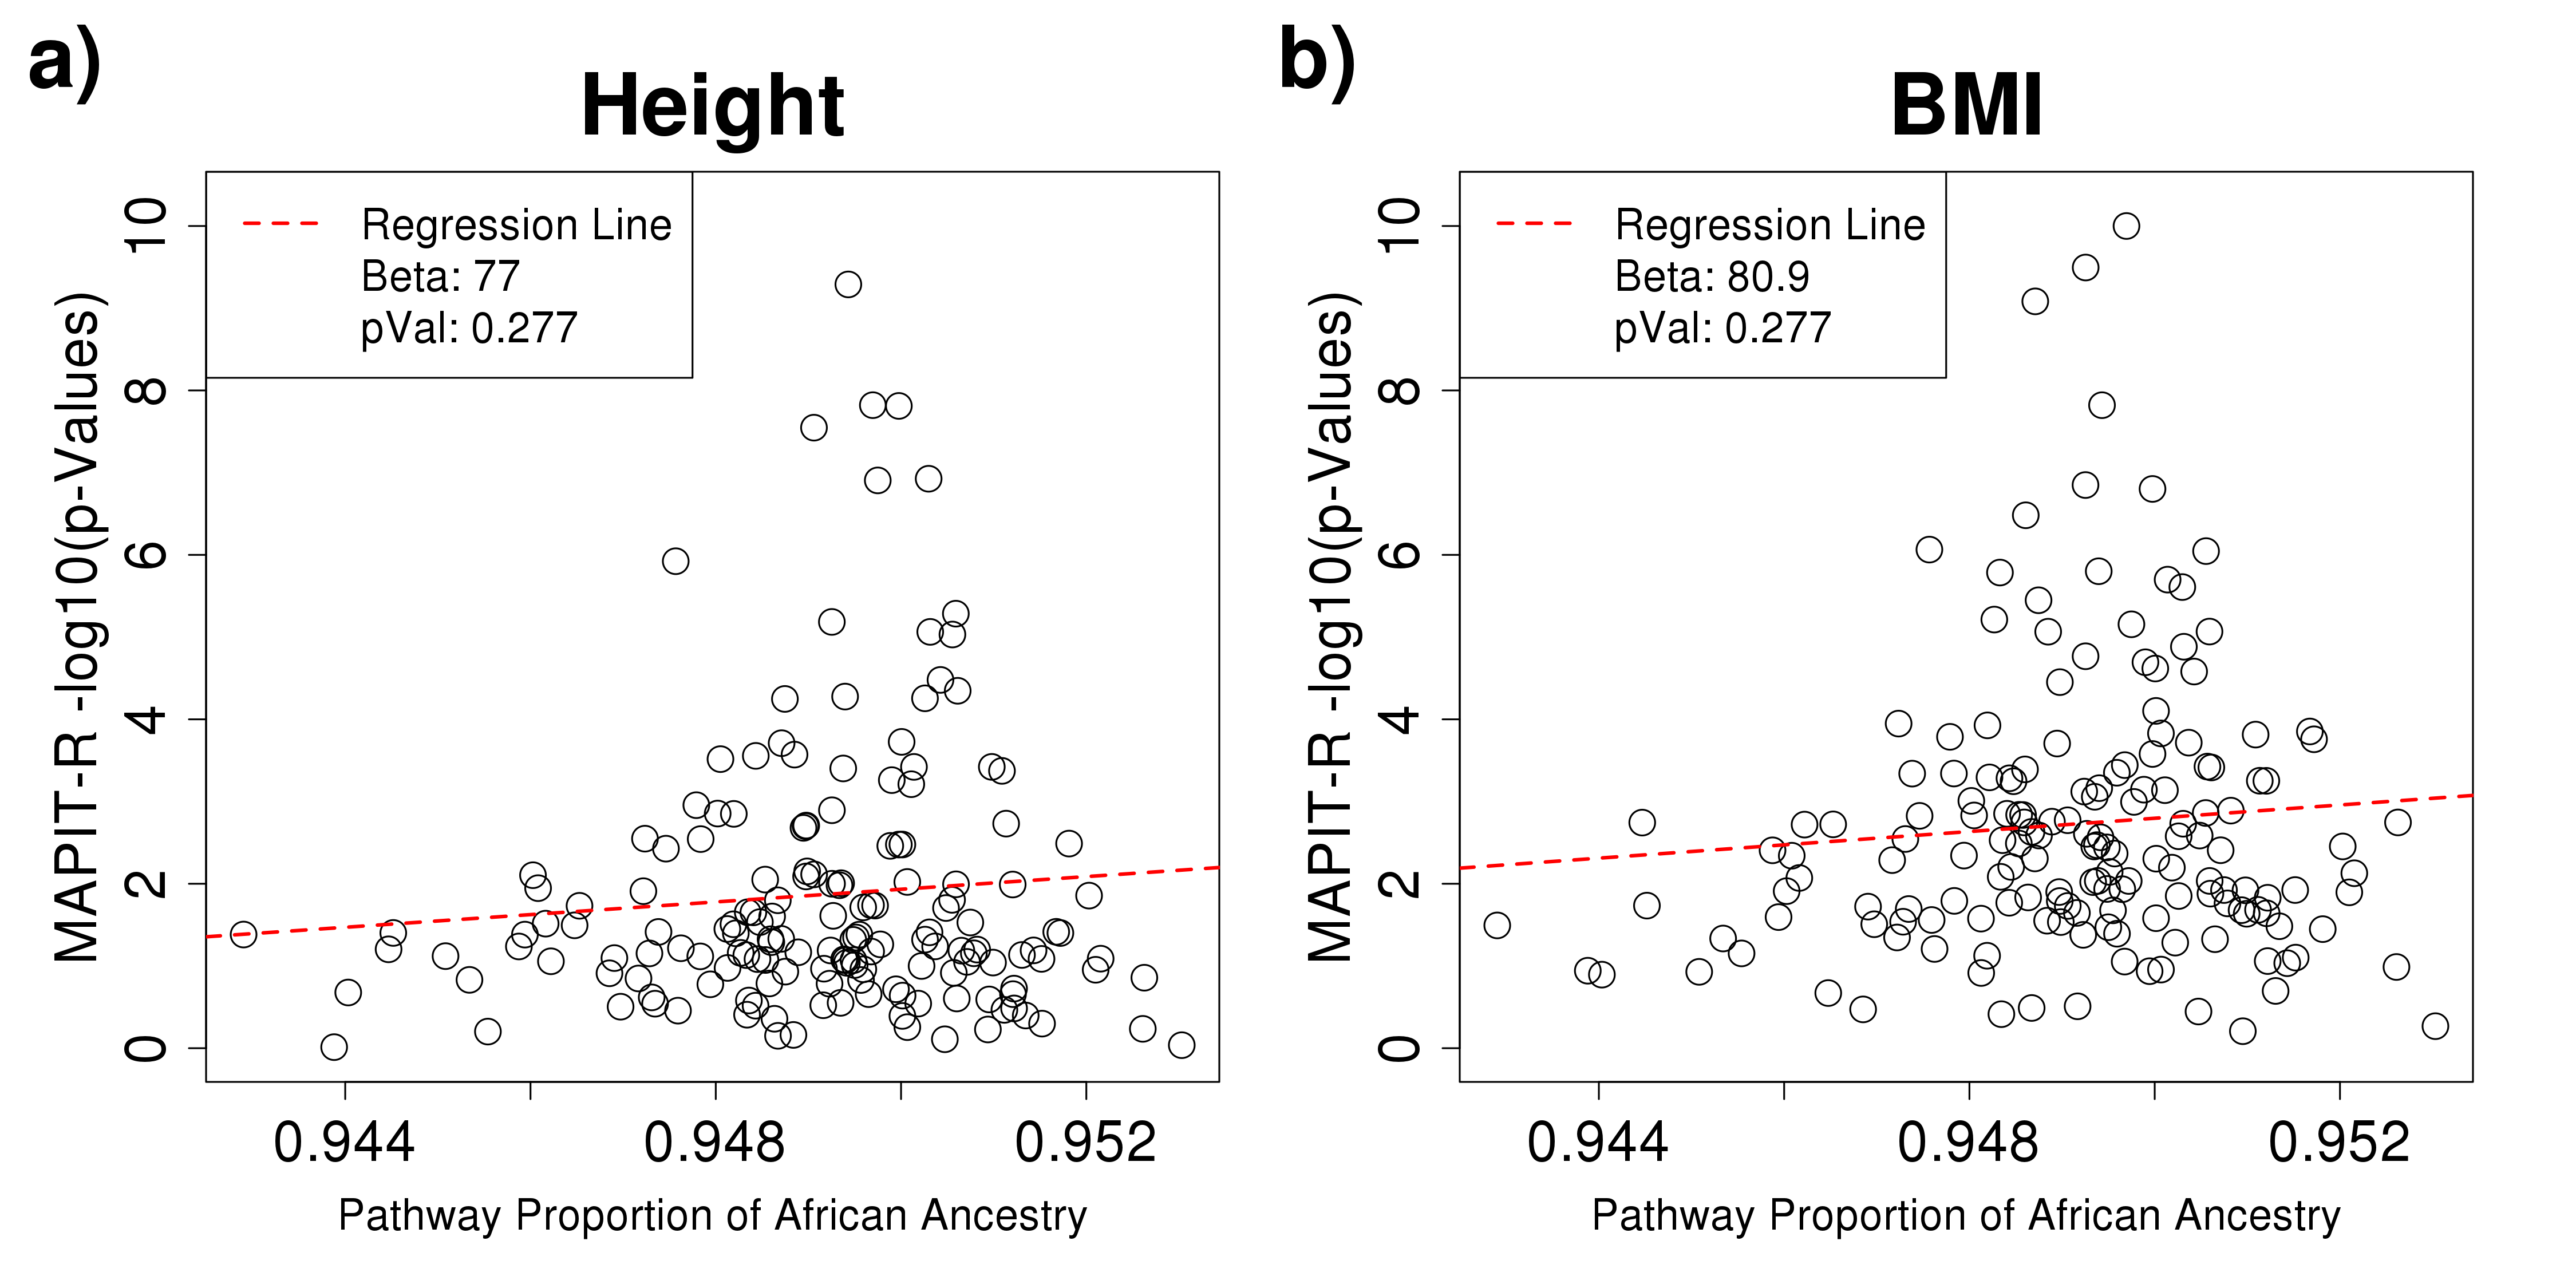
\includegraphics[scale=.35]{Images/Supp/InterPath_Supp_Figure_RFMix_vs2_African_KEGG_noHLA.png}
\caption[TBD]{\textbf{Pathway-level genetic diversity vs. MAPIT-R results in the African subgroup and KEGG database}. The figure shows the mean pairwise IBS proportions per pathway plotted against each pathway's MAPIT-R $p$-value for the African subgroup KEGG (a) height and (b) BMI analysis. IBS proportions were calculated per pathway by using each pathway's set of SNPs to derive pairwise IBS values between every set of individuals in the subgroup, and then averaging across each of these pairs for a final summary metric. Results with REACTOME database pathways can be found in Supplementary Figure \ref{InterPath-Main-Figure-RFMix-African-REACTOME}. We observe across the majority of our combinations no significant relationship between a pathway's mean pairwise IBS proportion and its MAPIT-R $p$-value.}
\label{InterPath-Supp-Figure-RFMix-African-KEGG}
\end{figure}
\clearpage

\setlength{\footskip}{3cm}
\begin{figure}[htbp]
\centering
\vspace*{-2cm}
\includegraphics[scale=.2]{Images/Supp/InterPath_Supp_Figure_PC1Loading_AllPaths_vs2_noHLA.png}
\caption[TBD]{\textbf{Relationship between MAPIT-R $p$-values and proportions of pathway SNPs loaded on PC1, all pathways}. Caption continued on next page.}
\label{InterPath-Supp-Figure-PC1Loading-AllPaths}
\end{figure}
\clearpage
\setlength{\footskip}{1cm}

\addtocounter{figure}{-1}
\begin{figure} [t!]
  \caption{\textbf{Relationship between MAPIT-R $p$-values and proportions of pathway SNPs loaded on PC1, all pathways}. The figure shows the proportion of SNPs within a given pathway that are strongly loaded on local PC1 plotted against that pathway's MAPIT-R -$\log_{10}$ $p$-value. All pathway sizes were used for this analysis. `Local' here refers to PCA having been conducted within-subgroup. SNPs are designated as `strongly loaded' on local PC1 if they are within the 10\% tails of the loading SNP score distributions. We observe that there is no significantly positive relationship between MAPIT-R $p$-values and proportion of SNPs that are strongly loaded on PC1 for any pathway database-phenotype-subgroup combination.}
\label{InterPath-Supp-Figure-PC1Loading-AllPaths-Caption}
\end{figure}
\clearpage

\setlength{\footskip}{2cm}
\begin{figure}[htbp]
\centering
\vspace*{-1.75cm}
\hspace*{-1cm}
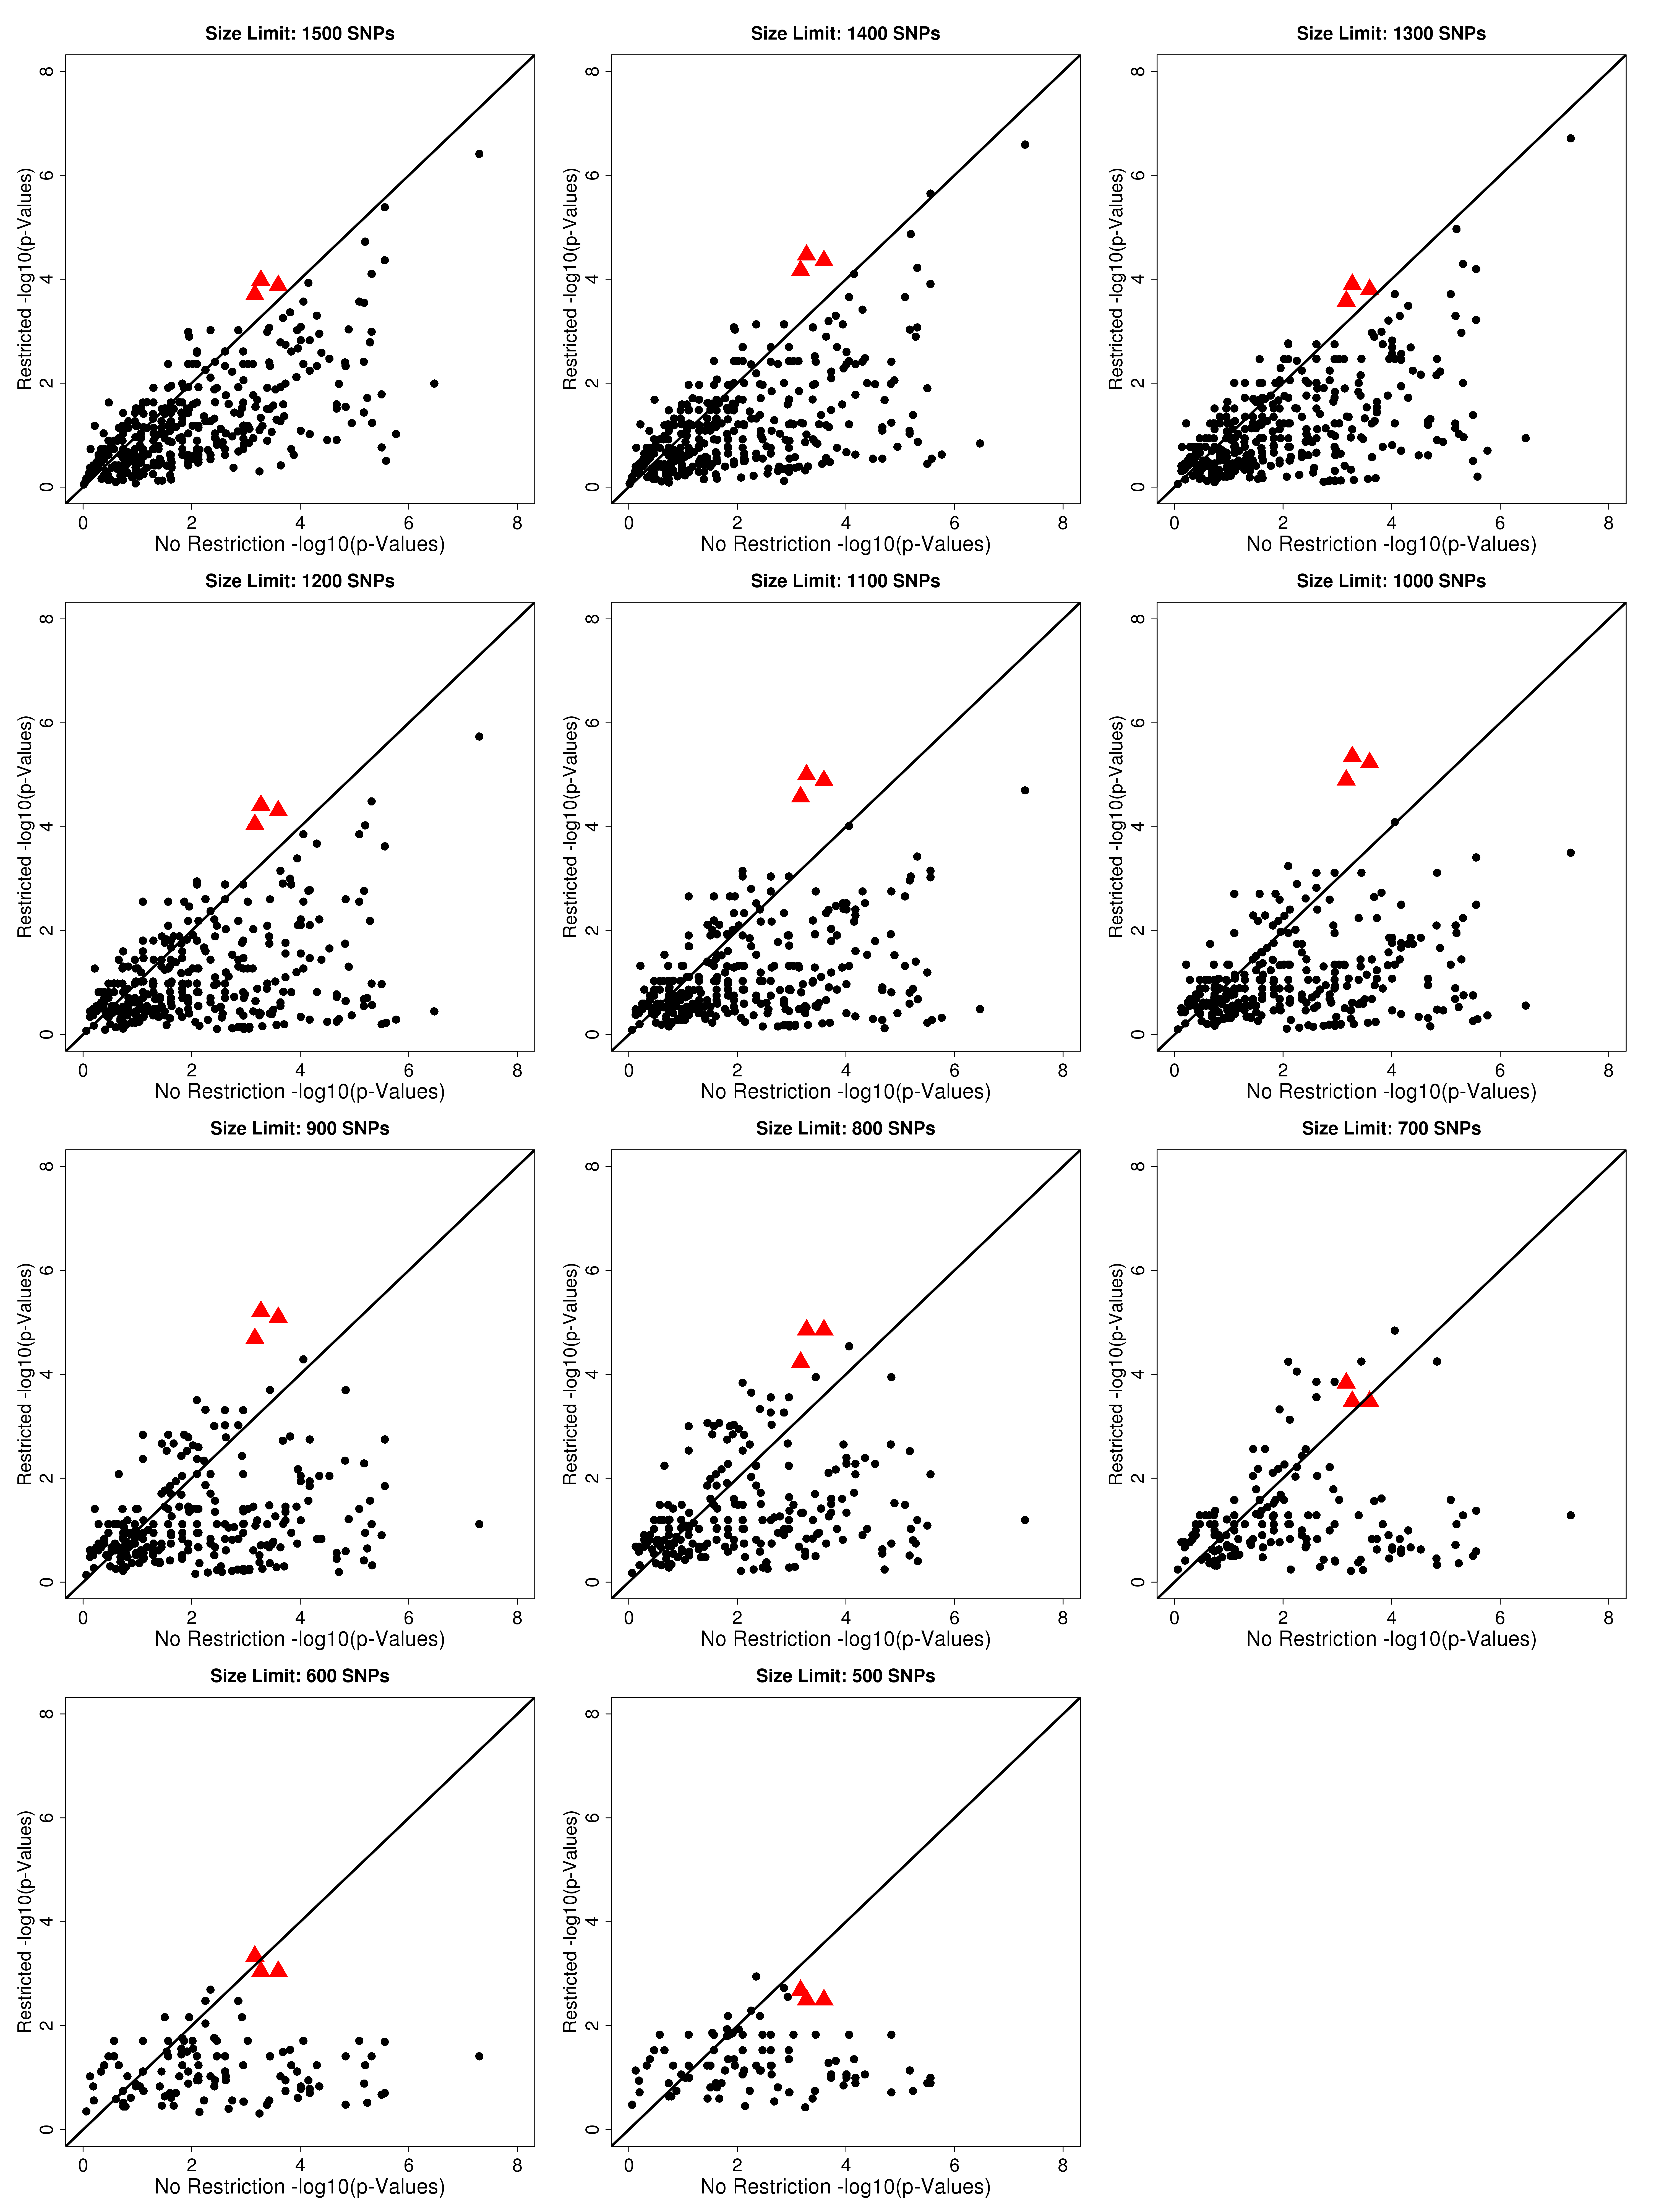
\includegraphics[scale=.325]{Images/Supp/InterPath_Supp_Figure_Hypergemeotric_SizeThresholds_vs1.png}
\caption[TBD]{\textbf{Impact of pathway size thresholds on hypergeometric enrichment analyses}. Caption continued on next page.}
\label{InterPath-Supp-Figure-Hypergeoemtric-SizeThresholds}
\end{figure}
\clearpage
\setlength{\footskip}{1cm}

\addtocounter{figure}{-1}
\begin{figure} [t!]
  \caption{\textbf{Impact of pathway size thresholds on hypergeometric enrichment analyses}. The figure shows multiple comparisons of size-restricted hypergeometric enrichment analyses versus unrestricted hypergeometric enrichment analyses using incrementally decreasing pathway size thresholds. Size thresholds change from 1,500 SNPs to 500 SNPs in 100 SNP increments. In each plot the $x$-axis is the unrestricted hypergeometric $p$-value for each gene and the $y$-axis is the size-restricted hypergeometric $p$-value for each gene. Red triangles represent results for each gene belonging to a proteasome gene family ({\emph{PSMA}}, {\emph{PSMB}}, {\emph{PSMC}}, {\emph{PSMD}}, {\emph{PSME}}, and {\emph{PSMF}}). Note that there are only three triangles since most proteasome genes are assigned to the same pathways.}
\label{InterPath-Supp-Figure-Hypergeoemtric-SizeThresholds-Caption}
\end{figure}
\clearpage

\section{Supplementary Tables}\label{Supplementary-Tables}

\begin{table}[ht]
\centering
\begin{tabular}{ccccc}
  \hline
\textbf{UK BioBank} & \textbf{Individuals} & \textbf{SNPs} & \textbf{KEGG} & \textbf{REACTOME} \\
\textbf{subgroup} & & & \textbf{Pathways} & \textbf{Pathways}  \\
  \hline
\textbf{Original subgroups:} & & & & \\
African & 3111 & 374466 & 180 & 658 \\ 
British.Ran4000 & 3848 & 600006 & 173 & 650 \\ 
Caribbean & 3833 & 410017 & 181 & 661 \\ 
Chinese & 1448 & 345221 & 153 & 626 \\ 
Indian & 5077 & 505854 & 181 & 662 \\ 
Pakistani & 1581 & 516806 & 141 & 596 \\ 
\\
\textbf{British Replicates:} & & & & \\
British.Ran4000.2 & 3869 & 599381 & 173 & 650 \\ 
British.Ran4000.3 & 3836 & 600654 & 173 & 649 \\ 
British.Ran4000.4 & 3838 & 599829 & 173 & 650 \\ 
British.Ran4000.5 & 3853 & 599442 & 173 & 650 \\ 
British.Ran10000 & 9603 & 597298 & 186 & 669 \\ 
British.Ran10000.2 & 9628 & 597577 & 186 & 669 \\ 
British.Ran10000.3 & 9636 & 597486 & 186 & 669 \\ 
British.Ran10000.4 & 9593 & 597369 & 186 & 669 \\ 
British.Ran10000.5 & 9596 & 597507 & 186 & 669 \\ 
  \hline
\end{tabular}
\caption[TBD]{\textbf{Pathways and subgroups of the UK BioBank analyzed in this study}. The table shows the individual, SNP, and pathway counts for each of the UKB subgroups analyzed in this study. `Original subgroups' refers to the multiple global human ancestries that were initially analyzed at the beginning of this study, and `British Replicates' refers specifically to the subgroups that were created to analyze multiple, independent random subsamples of the UKB British cohort. The number of individuals and SNPs post quality-control are shown in the second and third columns (see Materials and Methods), and the number of KEGG and REACTOME pathways analyzed in each subgroup are shown in the fourth and fifth columns. Note that for the `British Replicates' subgroups each group began with an independent set of either 4,000 or 10,000 individuals from the original UKB phenotype file.}
\label{InterPath-Supp-Table-UKBPopStats}
\end{table}
\clearpage

%Irish & 11575 & 588324 & 186 & 671 \\ 

%\textbf{Supplementary Tables 2a-d.} \textbf{Lists of New \bmass{} Multivariate Associations, per Dataset}. \\ Attached Excel sheets list new \bmass{} associations for each dataset analyzed.
%\bigskip \bigskip

\begin{table} [t!]
  \caption{\textbf{Lists of genome-wide significant MAPIT-R pathways, per subgroup}.  Attached Excel sheets list the pathways that were found to be MAPIT-R genome-wide significant in each UKB subgroup for the following phenotype and pathway database combinations: (a) KEGG+Height, (b) KEGG+BMI, (c) REACTOME+Height, and (d) REACTOME+BMI. Genome-wide significance was determined by using a Bonferroni-corrected $p$-value threshold of .05 divided by the number of pathways tested (Supplementary Table \ref{InterPath-Supp-Table-UKBPopStats}).}
\label{InterPath-Supp-Table-TopPathways-AllPaths-AllPhenos}
\end{table}
\clearpage

\setlength{\footskip}{4cm}
\begin{landscape}
\begin{table}[ht]
\vspace*{-1.5cm}
\centering
\hspace*{-3.5cm}
\begin{tabular}{ccccccccc}
  \hline
\textbf{Population} & \textbf{Pathway} & \textbf{Bonferroni} & \textbf{Bonferroni} & \textbf{Bonferroni} & \multicolumn{2}{c}{\textbf{.001 Threshold}} & \multicolumn{2}{c}{\textbf{.01 Threshold}} \\
\cline{6-7}
\cline{8-9}
 & \textbf{Counts} & \textbf{Threshold} & \textbf{Counts} & \textbf{FDR} & \textbf{Counts} & \textbf{FDR} & \textbf{Counts} & \textbf{FDR} \\ 
  \hline
\textbf{KEGG Height:} & & & & & & & \\
African & 1800 & 2.778E-04 & 0 & 0.000  & 1 & 0.056 & 10 & 0.556 \\ 
  British.Ran4000 & 1730 & 2.890E-04 & 0 & 0.000 & 0 & 0.000 & 13 & 0.751 \\ 
  Caribbean & 1810 & 2.762E-04 & 1 & 0.055 & 1 & 0.055 & 5 & 0.276 \\ 
  Chinese & 1530 & 3.268E-04 & 0 & 0.000 & 3 & 0.196 & 24 & 1.569 \\ 
  Indian & 1810 & 2.762E-04 & 1 & 0.055 & 1 & 0.055 & 20 & 1.105 \\ 
  Pakistani & 1410 & 3.546E-04 & 0 & 0.000 & 2 & 0.142 & 17 & 1.206 \\ 
  \\
  \textbf{KEGG BMI:} & & & & & & & \\
African & 1800 & 2.778E-04 & 0 & 0.000 & 1 & 0.056 & 10 & 0.556 \\ 
  British.Ran4000 & 1730 & 2.890E-04 & 0 & 0.000 & 0 & 0.000 & 13 & 0.751 \\ 
  Caribbean & 1810 & 2.762E-04 & 1 & 0.055 & 1 & 0.055 & 5 & 0.276 \\ 
  Chinese & 1530 & 3.268E-04 & 0 & 0.000 & 3 & 0.196 & 24 & 1.569 \\ 
  Indian & 1810 & 2.762E-04 & 1 & 0.055 & 1 & 0.055 & 20 & 1.105 \\ 
  Pakistani & 1410 & 3.546E-04 & 0 & 0.000 & 2 & 0.142 & 17 & 1.206 \\ 
  \\
  \textbf{REACTOME Height:} & & & & & & & \\
  African & 1800 & 2.778E-04 & 0 & 0.000 & 1 & 0.056 & 16 & 0.889 \\
  British.Ran4000 & 1730 & 2.890E-04 & 1 & 0.058 & 2 & 0.116 & 14 & 0.809 \\
  Caribbean & 1810 & 2.762E-04 & 0 & 0.000 & 1 & 0.055 & 25 & 1.381 \\
  Chinese & 1530 & 3.268E-04 & 0 & 0.000 & 1 & 0.065 & 24 & 1.569 \\
  Indian & 1810 & 2.762E-04 & 1 & 0.055 & 2 & 0.110 & 20 & 1.105 \\
  Pakistani & 1410 & 3.546E-04 & 0 & 0.000 & 2 & 0.142 & 15 & 1.064 \\
  \\
  \textbf{REACTOME BMI:} & & & & & & & \\
African & 6580 & 7.599E-05 & 1 & 0.015 & 4 & 0.061 & 39 & 0.593 \\
  British.Ran4000 & 6490 & 7.704E-05 & 1 & 0.015 & 4 & 0.062 & 52 & 0.801 \\
  Caribbean & 6610 & 7.564E-05 & 0 & 0.000 & 13 & 0.197 & 97 & 1.467 \\
  Chinese & 6260 & 7.987E-05 & 0 & 0.000 & 6 & 0.096 & 49 & 0.783 \\
  Indian & 6620 & 7.553E-05 & 0 & 0.000 & 3 & 0.045 & 66 & 0.997 \\
  Pakistani & 5960 & 8.389E-05 & 0 & 0.000 & 4 & 0.067 & 45 & 0.755 \\
   \hline
\end{tabular}
\caption[TBD]{\textbf{MAPIT-R false discovery rates at different significance thresholds, per subgroup}. Caption continued on next page. }
\label{InterPath-Supp-Table-AllPops-FDRs}
\end{table}
\end{landscape}
\clearpage
\setlength{\footskip}{1cm}

\addtocounter{table}{-1}
\begin{table} [t!]
  \caption{\textbf{MAPIT-R false discovery rates at different significance thresholds, per subgroup}. The table shows for various significance thresholds the false discovery rates observed from MAPIT-R when run on ten rounds of phenotype permutations for each UKB subgroup and pathway database. The first column lists the pathway database-phenotype-UKB subgroup combinations. The second column lists the total number of pathways that were tested across each of the ten phenotype permutations. The third column shows the $p$-value threshold associated with using the Bonferroni method of correction, also known as the `genome-wide significant' threshold. The fourth column shows the number of pathways across all ten phenotype permutation rounds that crossed this Bonferroni threshold. The fifth column shows the associated FDR associated with the fourth column. And the remaining six columns show the same setup as columns three to five but with a $p$-value threshold of either 0.001 or 0.01.}
\label{InterPath-Supp-Table-AllPops-FDRs-Caption}
\end{table}
\clearpage

\setlength{\footskip}{2cm}
\begin{landscape}
\begin{table}[ht]
\centering
\begin{tabular}{ll}
  \hline
 \textbf{Population} & \textbf{Pathways}\\
 \textbf{Comparison} & \\
  \hline
\textbf{African Vs.} & \\
\textbf{Caribbean:} & \\
 & KEGG\_ARRHYTHMOGENIC\_RIGHT\_VENTRICULAR\_CARDIOMYOPATHY\_ARVC \\
 & KEGG\_AXON\_GUIDANCE \\
 & KEGG\_CHEMOKINE\_SIGNALING\_PATHWAY \\
 & KEGG\_HYPERTROPHIC\_CARDIOMYOPATHY\_HCM \\
 & KEGG\_NATURAL\_KILLER\_CELL\_MEDIATED\_CYTOTOXICITY \\
 & KEGG\_VASCULAR\_SMOOTH\_MUSCLE\_CONTRACTION \\
\\
\textbf{African Vs.} & \\
\textbf{Chinese:} & \\
 & KEGG\_ALLOGRAFT\_REJECTION \\
 & KEGG\_ANTIGEN\_PROCESSING\_AND\_PRESENTATION \\
 & KEGG\_GRAFT\_VERSUS\_HOST\_DISEASE \\
 & KEGG\_SYSTEMIC\_LUPUS\_ERYTHEMATOSUS \\
 & KEGG\_TYPE\_I\_DIABETES\_MELLITUS \\
   \hline
\end{tabular}
\caption[TBD]{\textbf{Genome-wide significant MAPIT-R KEGG pathway overlap between UKB subgroups, in height}. Caption continued on next page. }
\label{InterPath-Supp-Table-MAPITR-TopPathway-Overlap}
\end{table}
\end{landscape}
\clearpage
\setlength{\footskip}{1cm}

\addtocounter{table}{-1}
\begin{table} [t!]
  \caption{\textbf{Genome-wide significant MAPIT-R KEGG pathway overlap between UKB subgroups, in height}. The table shows genome-wide significant pathways that overlap between multiple UKB subgroups. Specifically, pathways that overlap between the African subgroup and Caribbean subgroup, and between the African subgroup and Chinese subgroup, are listed for height results from KEGG.}
\label{InterPath-Supp-Table-MAPITR-TopPathway-Overlap-Caption}
\end{table}
\clearpage

\setlength{\footskip}{2cm}
\begin{table}[ht]
\centering
\begin{tabular}{lll}
  \hline
 \textbf{Population} & \textbf{Gene} & \textbf{Genes} \\
 \textbf{Comparison} & \textbf{Count} & \\
  \hline
\textbf{African Vs.} & & \\
\textbf{Caribbean:} & & \\
& 4 & MAPK3,MAPK1 \\
& 3 & ROCK2,ROCK1,RHOA,RAF1,RAC2,RAC1,PRKCB, \\
& & PAK1,NRAS,MAP2K1,KRAS,ITGB1,HRAS,CACNA1S, \\
& & CACNA1D,CACNA1C,BRAF \\
\\
\textbf{African Vs.} & & \\
\textbf{Chinese:} & & \\
& 5 & HLA-DRB1,HLA-DRA,HLA-DQB1,HLA-DQA2,HLA-DQA1, \\
& & HLA-DPB1,HLA-DPA1,HLA-DOB,HLA-DOA,HLA-DMB, \\
& & HLA-DMA \\
& 4 & TNF,IFNG,HLA-G,HLA-F,HLA-E,HLA-C,HLA-B,HLA-A, \\ 
& & CD86,CD80,CD28 \\
& 3 & PRF1,IL2,GZMB,FASLG,FAS \\
   \hline
\end{tabular}
\caption[TBD]{\textbf{Gene counts across genome-wide significant MAPIT-R KEGG pathways that overlap between UKB subgroups, in height}. The table shows genes that are present across multiple pathways that overlap between the population subgroups referenced in the first column. Pathways from which these gene count lists are derived can be found in Supplementary Table \ref{InterPath-Supp-Table-MAPITR-TopPathway-Overlap}. The second column lists the number of times the given genes appear across the aforementioned lists of pathways. The third column lists the specific genes the appear at the specific gene count numbers. Note that these results are specifically for the KEGG height analysis.}
\label{InterPath-Supp-Table-MAPITR-TopPathway-GeneCounts-Overlap}
\end{table}
\clearpage
\setlength{\footskip}{1cm}

\begin{table}[ht]
\centering
\begin{tabular}{cl}
  \hline
 \textbf{Frequency} & \textbf{Genes} \\
  \hline
  4 & PIK3R5,PIK3R3,PIK3R2,PIK3R1,PIK3CG,PIK3CD,PIK3CB, \\
  & PIK3CA,AKT3,AKT2,AKT1 \\
  3 & SOS2,SOS1,RAF1,PLCG1,NRAS,MAPK3,MAPK1,MAP2K2, \\
  & MAP2K1,KRAS,HRAS,GRB2,CDK4 \\
  2 & TP53,TGFA,RXRG,RXRB,RXRA,RELA,RB1,RARB,PTK2, \\
  & PRKCG,PRKCB,PRKCA,PLCG2,PDPK1,PAK6,PAK4,PAK2, \\
  & PAK1,NFKBIA,NFKB1,NCK2,NCK1,MYC,MAPK9,MAP2K7, \\ 
  & JUN,IKBKB,GSK3B,FHIT,ERBB2,EGFR,EGF,E2F3,E2F2, \\
  & E2F1,CHUK,CDKN1B,CDK6,CCND1,CBLC,CBLB,CBL, \\
  & CASP9,BRAF,BAD \\
   \hline
\end{tabular}
\caption[TBD]{\textbf{Gene counts across four KEGG pathways highlighted in African height vs. BMI analysis (Figure \ref{InterPath-Main-Figure-MAPITR-PhenoComps-African})}. The table shows the genes that are present across multiple of the pathways highlighted in blue in Figure \ref{InterPath-Main-Figure-MAPITR-PhenoComps-African}; these are pathways that have particularly more significant MAPIT-R $p$-values in BMI than in height. The first column lists the frequency (out of four) the given genes appear across the aforementioned list of pathways in Figure \ref{InterPath-Main-Figure-MAPITR-PhenoComps-African}. The second column lists the specific genes that appear at the given frequency across the four pathways highlighted in Figure \ref{InterPath-Main-Figure-MAPITR-PhenoComps-African}.}
\label{InterPath-Supp-Table-MAPITR-PhenoComps-African-GeneCounts}
\end{table}
\clearpage

\begin{table} [t!]
  \caption{\textbf{Gene counts across MAPIT-R genome-wide significant pathways, per subgroup}. Attached Excel sheets contain lists of genes that appear multiple times across the MAPIT-R genome-wide significant pathways in each UKB subgroup for the following pathway database-phenotype combinations: (a) KEGG-Height, (b) KEGG-BMI, (c) REACTOME-Height, and (d) REACTOME-BMI. Genome-wide significance was determined by using a Bonferroni-corrected $p$-value threshold of .05 divided by the number of pathways tested (Supplementary Table \ref{InterPath-Supp-Table-UKBPopStats}).}
\label{InterPath-Supp-Table-AllPops-TopGeneCounts-Caption}
\end{table}

\begin{table} [t!]
  \caption{\textbf{Gene counts across size-restricted MAPIT-R genome-wide significant pathways, per subgroup}. Attached Excel sheets contain lists of genes that appear multiple times across the MAPIT-R genome-wide significant pathways that contain less than or equal to 1,000 SNPs (`size-restricted') in each UKB subgroup for the following pathway database-phenotype combinations: (a) KEGG-Height, (b) KEGG-BMI, (c) REACTOME-Height, and (d) REACTOME-BMI. Genome-wide significance was determined by using a Bonferroni-corrected $p$-value threshold of .05 divided by the number of pathways tested (Supplementary Table \ref{InterPath-Supp-Table-UKBPopStats}).}
\label{InterPath-Supp-Table-AllPops-TopGeneCounts-SizeRestricted-Caption}
\end{table}
\clearpage

\begin{table} [t!]
  \caption{\textbf{Results from original and size-restricted hypergeometric tests in BMI-African, per gene.}. Attached Excel sheets contain lists of the hypergeometric -$\log_{10}$ $p$-values for both the original and size-restricted gene count analyses per gene in both the KEGG and REACTOME-BMI-African combinations. Differences in the -$\log_{10}$ $p$-values between the original and size-restricted hypergeometric analyses are also shown per gene. Plots of these differences in -$\log_{10}$ $p$-values can be seen in Figure \ref{InterPath-Main-Figure-Hypergeometric-RestrictedComps-African-BMI}.}
\label{InterPath-Supp-Table-Hypergeometric-RestrictedComps-African-BMI}
\end{table}
\clearpage

\begin{landscape}
\begin{table}[ht]
\centering
\hspace*{-1.5cm}
\begin{tabular}{ccccccc}
  \hline
  \textbf{Gene} & \textbf{Pathway SNP} & \textbf{Gene Count in} & \textbf{Total Count of} & \textbf{Gene Count in} & \textbf{Total Count of} & \textbf{Hypergeometric} \\
   & \textbf{Count Limit} & \textbf{Top Pathways} & \textbf{Top Pathways} & \textbf{All Pathways} & \textbf{All Pathways} & \textbf{$p$-Value} \\
  \hline
 \textbf{UBA52} & & & & & & \\
 & No Limit & 22 & 65 & 106 & 658 & 1.537E-4 \\
 & $<$ 1000 SNPs & 10 & 26 & 84 & 577 & 1.855E-3 \\
\\
 \textbf{PSM*} & & & & & & \\
 & No Limit & 12 & 65 & 44 & 658 & 5.304E-4 \\
 & $<$ 1000 SNPs & 9 & 26 & 34 & 577 & 4.464E-6 \\
   \hline
\end{tabular}
\caption[TBD]{\textbf{MAPIT-R Genome-Wide Significant Pathway Gene Counts: Hypergeometric Enrichment Examples}. Caption continued on next page.}
\label{InterPath-Supp-Table-AllPops-TopGeneCount-HypergeometricTests}
\end{table}
\end{landscape}
\clearpage

\addtocounter{table}{-1}
\begin{table} [t!]
  \caption{\textbf{PSM* and UBA52 gene count enrichment test examples, size restriction and no restriction}. The table shows examples and results of running the hypergeometric test for enrichment on two different genes in two different study designs. In all cases a gene is tested for being significantly more frequent among the set of MAPIT-R genome-wide significant pathways than among the background distribution of pathways in the original database. Two study designs were employed for these tests, either (a) using all pathways present in the given databases or (b) using only pathways that contained less than or equal to 1,000 SNPs. The first column lists the gene or gene family being tested. The second column lists which of the two aforementioned study designs was used. Columns three through six list the different count values used in the hypergeometric test: the third column lists the number of times a gene is present among the genome-wide significant list of pathways, the fourth column lists the total number of pathways that were genome-wide significant, the fifth column lists the number of times a gene is present among all the pathways in the given database, and the sixth column lists the total number of pathways in the given database. The seventh column is the hypergeometric $p$-value associated with columns three through six. Note that the vast majority of proteasome genes included in our analysis had the same number of gene counts across each hypergeometric category, hence why \textbf{PSM*} was used to represent them as a whole.}
\label{InterPath-Supp-Table-AllPops-TopGeneCount-HypergeometricTests-Caption}
\end{table}
\clearpage

\begin{table} [t!]
  \caption{\textbf{MAPIT-R $p$-values from rerunning REACTOME pathways + BMI with each proteasome gene family individually removed, per subgroup}. Attached Excel sheets contain the MAPIT-R $p$-values for each of the REACTOME pathways analyzed in Figure \ref{InterPath-Main-Figure-Proteasome-Panels} + BMI with each of the proteasome gene families (eg \textit{PSMA}, \textit{PSMB}, \textit{PSMC}, \textit{PSMD}, \textit{PSME}, and \textit{PSMF}) removed one at a time, per UKB subgroup. These are the raw MAPIT-R $p$-values underlying Figure \ref{InterPath-Main-Figure-Proteasome-Panels} and Supplementary Figures \ref{InterPath-Supp-Figure-Prot-Heatplots-African}\textcolor{blue}{-f}. Note that for some subgroups not all of the original pathways from Figure \ref{InterPath-Main-Figure-Proteasome-Panels} were analyzable (generally due to number of SNPs >> number of individuals).}
\label{InterPath-Supp-Table-AllPops-Proteasome-Dropouts-Caption}
\end{table}
\clearpage

\setlength{\footskip}{4cm}
\begin{landscape}
\begin{table}[ht]
\vspace*{-1.25cm}
\centering
\hspace*{-3.25cm}
\begin{tabular}{ccccccccccc}
  \hline
\textbf{Population} & \textbf{Pathway} & \textbf{Bonferroni} & \textbf{Bonferroni} & \textbf{Bonferroni} & \textbf{0.001} & \textbf{0.001} & \textbf{0.001} & \textbf{0.01} & \textbf{0.01} & \textbf{0.01} \\
 & \textbf{Counts} & \textbf{Threshold} & \textbf{Counts} & \textbf{FDR} & \textbf{Threshold} & \textbf{Counts} & \textbf{FDR} & \textbf{Threshold} & \textbf{Counts} & \textbf{FDR} \\ 
  \hline
\textbf{KEGG Height:} & & & & & & & & & \\
British.Ran4000 & 1730 & 2.890E-04 & 0 & 0.000 & 0.001 & 0 & 0.000 & 0.010 & 13 & 0.751 \\
  British.Ran4000.2 & 1730 & 2.890E-04 & 0 & 0.000 & 0.001 & 1 & 0.058 & 0.010 & 18 & 1.040 \\
  British.Ran4000.3 & 1730 & 2.890E-04 & 1 & 0.058 & 0.001 & 1 & 0.058 & 0.010 & 20 & 1.156 \\
  British.Ran4000.4 & 1730 & 2.890E-04 & 0 & 0.000 & 0.001 & 4 & 0.231 & 0.010 & 23 & 1.329 \\
  British.Ran4000.5 & 1730 & 2.890E-04 & 0 & 0.000 & 0.001 & 2 & 0.116 & 0.010 & 22 & 1.272 \\
  British.Ran10000.1 & 1860 & 2.688E-04 & 0 & 0.000 & 0.001 & 1 & 0.054 & 0.010 & 26 & 1.398 \\
  British.Ran10000.2 & 1860 & 2.688E-04 & 0 & 0.000 & 0.001 & 1 & 0.054 & 0.010 & 12 & 0.645 \\
  British.Ran10000.3 & 1860 & 2.688E-04 & 2 & 0.108 & 0.001 & 2 & 0.108 & 0.010 & 21 & 1.129 \\
  British.Ran10000.4 & 1860 & 2.688E-04 & 1 & 0.054 & 0.001 & 2 & 0.108 & 0.010 & 16 & 0.860 \\
  British.Ran10000.5 & 1860 & 2.688E-04 & 0 & 0.000 & 0.001 & 0 & 0.000 & 0.010 & 12 & 0.645 \\
  \\
  \textbf{KEGG BMI:} & & & & & & & & & \\
British.Ran4000 & 1730 & 2.890E-04 & 1 & 0.058 & 0.001 & 2 & 0.116 & 0.010 & 14 & 0.809 \\
  British.Ran4000.2 & 1730 & 2.890E-04 & 0 & 0.000 & 0.001 & 1 & 0.058 & 0.010 & 23 & 1.329 \\
  British.Ran4000.3 & 1730 & 2.890E-04 & 0 & 0.000 & 0.001 & 3 & 0.173 & 0.010 & 21 & 1.214 \\
  British.Ran4000.4 & 1730 & 2.890E-04 & 1 & 0.058 & 0.001 & 5 & 0.289 & 0.010 & 21 & 1.214 \\
  British.Ran4000.5 & 1730 & 2.890E-04 & 2 & 0.116 & 0.001 & 7 & 0.405 & 0.010 & 23 & 1.329 \\
  British.Ran10000.1 & 1860 & 2.688E-04 & 0 & 0.000 & 0.001 & 1 & 0.054 & 0.010 & 25 & 1.344 \\
  British.Ran10000.2 & 1860 & 2.688E-04 & 2 & 0.108 & 0.001 & 4 & 0.215 & 0.010 & 22 & 1.183 \\
  British.Ran10000.3 & 1860 & 2.688E-04 & 0 & 0.000 & 0.001 & 2 & 0.108 & 0.010 & 20 & 1.075 \\
  British.Ran10000.4 & 1860 & 2.688E-04 & 1 & 0.054 & 0.001 & 2 & 0.108 & 0.010 & 23 & 1.237 \\
  British.Ran10000.5 & 1860 & 2.688E-04 & 0 & 0.000 & 0.001 & 0 & 0.000 & 0.010 & 20 & 1.075 \\
   \hline
\end{tabular}
\caption[TBD]{\textbf{MAPIT-R false discovery rates at different significance thresholds, per British replicate}. Caption continued at end of tables.}
\label{InterPath-Supp-Table-BritReps-FDRs-pt1}
\end{table}
\end{landscape}
\clearpage
\setlength{\footskip}{1cm}
\addtocounter{table}{-1}

\setlength{\footskip}{4cm}
\renewcommand{\thetable}{\arabic{table}}
\begin{landscape}
\begin{table}[ht]
\vspace*{-1.25cm}
\centering
\hspace*{-3.5cm}
\begin{tabular}{ccccccccccc}
  \hline
\textbf{Population} & \textbf{Pathway} & \textbf{Bonferroni} & \textbf{Bonferroni} & \textbf{Bonferroni} & \textbf{0.001} & \textbf{0.001} & \textbf{0.001} & \textbf{0.01} & \textbf{0.01} & \textbf{0.01} \\
 & \textbf{Counts} & \textbf{Threshold} & \textbf{Counts} & \textbf{FDR} & \textbf{Threshold} & \textbf{Counts} & \textbf{FDR} & \textbf{Threshold} & \textbf{Counts} & \textbf{FDR} \\ 
  \hline
  \textbf{REACTOME Height:} & & & & & & & & & \\
British.Ran4000 & 6500 & 7.692E-05 & 0 & 0.000 & 0.001 & 9 & 0.138 & 0.010 & 69 & 1.062 \\
  British.Ran4000.2 & 6500 & 7.692E-05 & 0 & 0.000 & 0.001 & 4 & 0.062 & 0.010 & 61 & 0.938 \\
  British.Ran4000.3 & 6490 & 7.704E-05 & 1 & 0.015 & 0.001 & 8 & 0.123 & 0.010 & 59 & 0.909 \\
  British.Ran4000.4 & 6500 & 7.692E-05 & 0 & 0.000 & 0.001 & 5 & 0.077 & 0.010 & 69 & 1.062 \\
  British.Ran4000.5 & 6500 & 7.692E-05 & 0 & 0.000 & 0.001 & 6 & 0.092 & 0.010 & 53 & 0.815 \\
   British.Ran10000.1 & 6690 & 7.474E-05 & 0 & 0.000 & 0.001 & 4 & 0.060 & 0.010 & 55 & 0.822 \\
  British.Ran10000.2 & 6690 & 7.474E-05 & 0 & 0.000 & 0.001 & 4 & 0.060 & 0.010 & 52 & 0.777 \\
  British.Ran10000.3 & 6690 & 7.474E-05 & 2 & 0.030 & 0.001 & 11 & 0.164 & 0.010 & 60 & 0.897 \\
  British.Ran10000.4 & 6690 & 7.474E-05 & 1 & 0.015 & 0.001 & 4 & 0.060 & 0.010 & 69 & 1.031 \\
  British.Ran10000.5 & 6690 & 7.474E-05 & 0 & 0.000 & 0.001 & 4 & 0.060 & 0.010 & 60 & 0.897 \\

  \\
  \textbf{REACTOME BMI:} & & & & & & & & & \\
British.Ran4000 & 6490 & 7.704E-05 & 1 & 0.015 & 0.001 & 4 & 0.062 & 0.010 & 52 & 0.801 \\
  British.Ran4000.2 & 6500 & 7.692E-05 & 1 & 0.015 & 0.001 & 14 & 0.215 & 0.010 & 63 & 0.969 \\
  British.Ran4000.3 & 6490 & 7.704E-05 & 0 & 0.000 & 0.001 & 5 & 0.077 & 0.010 & 79 & 1.217 \\
  British.Ran4000.4 & 6500 & 7.692E-05 & 2 & 0.031 & 0.001 & 6 & 0.092 & 0.010 & 61 & 0.938 \\
  British.Ran4000.5 & 6500 & 7.692E-05 & 0 & 0.000 & 0.001 & 7 & 0.108 & 0.010 & 73 & 1.123 \\
  British.Ran10000.1 & 6690 & 7.474E-05 & 2 & 0.030 & 0.001 & 10 & 0.149 & 0.010 & 73 & 1.091 \\
  British.Ran10000.2 & 6690 & 7.474E-05 & 0 & 0.000 & 0.001 & 3 & 0.045 & 0.010 & 42 & 0.628 \\
  British.Ran10000.3 & 6690 & 7.474E-05 & 1 & 0.015 & 0.001 & 10 & 0.149 & 0.010 & 74 & 1.106 \\
  British.Ran10000.4 & 6690 & 7.474E-05 & 0 & 0.000 & 0.001 & 7 & 0.105 & 0.010 & 65 & 0.972 \\
  British.Ran10000.5 & 6690 & 7.474E-05 & 0 & 0.000 & 0.001 & 5 & 0.075 & 0.010 & 57 & 0.852 \\
   \hline
\end{tabular}
\caption[TBD]{\textbf{MAPIT-R false discovery rates at different significance thresholds, per British replicate}. Continued.}
\label{InterPath-Supp-Table-BritReps-FDRs-pt2}
\end{table}
\end{landscape}
\clearpage
\setlength{\footskip}{1cm}

\addtocounter{table}{-1}
\begin{table} [t!]
  \caption{\textbf{MAPIT-R false discovery rates at different significance thresholds, per British replicate}. The tables show for various significance thresholds the false discovery rates observed from MAPIT-R when run on ten rounds of phenotype permutations for each British replicate subsample and pathway database. The first column lists the pathway database-phenotype-British replicate subsample combinations. The second column lists the total number of pathways that were tested across each of the ten phenotype permutations. The third column shows the $p$-value threshold associated with using the Bonferroni method of correction, also known as the `genome-wide significant' threshold. The fourth column shows the number of pathways across all ten phenotype permutation rounds that crossed this Bonferroni threshold. The fifth column shows the associated FDR associated with the fourth column. And the remaining six columns show the same setup as columns three to five but with a $p$-value threshold of either 0.001 or 0.01.}
\label{InterPath-Supp-Table-BritReps-FDRs-Caption}
\end{table}
\clearpage

\setlength{\footskip}{3.5cm}
\begin{landscape}
\begin{table}[ht]
\centering
\vspace{-1cm}
\hspace*{-2.5cm}
\begin{tabular}{ccccccccc}
  \hline
  \multicolumn{2}{c}{\textbf{Database-Phenotype}} & & & & & & & \\
  \cline{1-2}
  & \textbf{Subgroup} & \textbf{Pathway} & \textbf{Bonferroni} & \textbf{SNP1} & \textbf{Locus1} & \textbf{SNP2} & \textbf{Locus2} & \textbf{Epistasis} \\
  & & & \textbf{Threshold} & & & & & \textbf{$p$-Value}\\
  \hline
 \multicolumn{2}{l}{\textbf{KEGG-Height}} & & & & & & & \\
 & African & Phosphatidylinositol & 7.95E-11 & 10:134411966 & INPP5A & 21:43586397 & Intergenic & 2.81E-11 \\
 & & Signaling System & & & (Intronic) & & & \\
 & & & & & & & & \\
 \multicolumn{2}{l}{\textbf{REACTOME-Height}} & & & &  & & & \\
 & Caribbean & Signaling By & 4.63E-11 & 8:13404303 & DLC1 & 18:71234727 & Intergenic & 3.41E-11\\
 & & Rho GTPases & & & (Intronic) & & & \\
 & & & & & &  & & \\
 \multicolumn{2}{l}{\textbf{REACTOME-BMI}} & & &  & & & & \\
 & African & Glycerophospholipid & 1.49E-10 & 12:14693353 &  PLBD1 & 4:129890790 & SCLT1 & 1.24E-10 \\
 & & Biosynthesis & & & (Intronic) & & (Intronic) & \\
 & & Assembly of the & 4.04E-10 & 22:35797833 &  MCM5 & 22:23489042 & RAB36 & 3.55E-10 \\
 & & Pre Replicative Complex & & & (Intronic) & & (Intronic) & \\
 & & Integrin Cell & 8.38E-11 & 17:45320514 &  ITGB3 & 6:25897169  & Intergenic & 7.85E-11 \\
 & & Surface Interactions & & & (Downstream) & & & \\ 
   \hline
\end{tabular}
\caption[TBD]{\textbf{Significant pairwise SNP interactions between MAPIT-R pathways and the rest of the genome}. The table shows pairwise SNP interactions that have $p$-values lower than Bonferroni-corrected thresholds for test schemes using MAPIT-R significant pathways versus the rest of the genome. Specifically, for every MAPIT-R significant pathway previously found in each pathway database-phenotype-subgroup combination (Supplementary Table \ref{InterPath-Supp-Table-TopPathways-AllPaths-AllPhenos}), all the SNPs within each pathway were tested for pairwise interactions with all the remaining SNPs in the genome using the PLINK v1.90b4 `\texttt{-{}-epistasis set-by-all'} command \cite{Purcell2007}. The first column shows the database-phenotype-subgroup combination specific for the given pathway, the second column shows the pathway containing the significant SNP pairwise interaction, the third column shows the Bonferroni corrected $p$-value threshold for significance (ie .05 / the number of pairwise tests that were conducted within the given pathway), the fourth column shows the SNP within the pathway that is part of the significant interaction (chromosome:basepair formatting), the fifth column shows the locus SNP1 maps to (if known), the sixth column shows the SNP from the rest of the genome that is the other part of the significant interaction (chromosome:basepair formatting), the seventh column shows the locus SNP2 maps to (if known) , and the eighth column shows the $p$-value for the PLINK pairwise epistasis test between SNP1 and SNP2. Combinations involving KEGG-BMI are not shown since no significant pairwise epistatic interactions were found with those groupings.}
\label{InterPath-Supp-Table-PairwiseEpi-Results}
\end{table}
\end{landscape}
\setlength{\footskip}{1cm}
\clearpage


\begingroup
\addcontentsline{toc}{section}{References}
%\bibliographystyle{apalike}
\setstretch{1.0}
\bibliography{Main}
\endgroup



\iffalse

SCRAP




\fi

\end{document}
